% !TeX spellcheck = en_GB
\chapter{String-net models for unitary fusion categories}
\label{ch:LW}

In the study of microscopic models for fusion categories we are not limited to one-dimensional systems. There is also a prominent example of a two-dimensional lattice model for the study of topologically ordered systems, namely the \emph{Levin-Wen model} \cite{Levin2005}. Although it is possible to define this model for any lattice form, it is usually discussed for the honeycomb lattice, which goes well with the structure of fusion categories since it only consists of trivalent vertices. The Levin-Wen model itself yields a Topological Quantum Field Theory (TQFT), but it is also a powerful tool in our search for a Conformal Field Theory (CFT) corresponding to the Haagerup subfactor.  Firstly, it requires as input a unitary fusion category, which is exactly the kind of category we get from a subfactor. Secondly, the quantum double of the category (which is the most promising candidate for finding a CFT) arises naturally in terms of the excitations of the Hamiltonian of the Levin-Wen model. Hence, calculating the excitations of the model yields a unitary modular tensor category, which, in turn, can then be studied in terms of anyon chains in order to find the corresponding CFT (as explained in \cref{sec:anyons}).

Even though this approach seams promising, there is one caveat: In the original paper by Levin and Wen the category does not only need to be a unitary fusion category, but the $F$-symbols of the category have to fulfil an additional constraint called \emph{tetrahedral symmetry}. However, not every unitary fusion category does fulfil this constraint. Several counterexamples are known (see for example \cite{Hong2009}), most importantly the Haagerup fusion category $\Hd$. However, the tetrahedral symmetry condition is not crucial for the model to work which was pointed out for example in \cite{Hong2009}, hence it is possible to construct a Hamiltonian in the sense of Levin and Wen from a unitary fusion category that does not fulfil tetrahedral symmetry.

In this chapter, we first elaborate on the tetrahedral symmetry condition and the connection of the Levin-Wen model to Turaev-Viro state sums, a mathematical theory that is equivalent to the Levin-Wen model but naturally circumvents the problem of tetrahedral symmetry. We then present the Levin-Wen model, first in its original form where tetrahedral symmetry holds before we show the construction without this constraint in detail. We also prove that the resulting Hamiltonian has the same properties as the original one and, furthermore, that it can be transformed into the original one when imposing tetrahedral symmetry. We then discuss how the excitations of the model can be computed and why this is especially difficult in the general approach where tetrahedral symmetry does not hold. Here, once again tensor networks will come into play as a practical tool for the investigation of physical systems. We show how to express the ground state of the Levin-Wen model as a tensor network for fusion categories without tetrahedral symmetry. In the end, we elaborate on possible generalisations of the model, namely either losing the constraint that the fusion rules are multiplicity-free or the constraint that the fusion category is unitary. While the first one is a true (but tedious) generalisation of the construction, the second one leads to unphysical models.

\newpage
\section{Tetrahedral symmetry}
\label{sec:tetrahedral}

%Recall that the matrix elements of the $F$-symbols are given by the equation
%	\begin{equation}
%		\begin{tikzpicture}[baseline=(current bounding box.center),yscale=0.9,xscale=0.9]
%			\draw (0,0.5) -- (0,1);
%			\draw (0,1) -- (-0.5,1.5);
%			\draw (-0.5,1.5) -- (-1,2);
%			\draw (-0.5,1.5) -- (0,2);
%			\draw (0,1) -- (0.5,1.5);
%			\draw (0.5,1.5) -- (1,2);
%			\node at (0,0.25) {\small $u$};
%			\node at (-1,2.25) {\small $a$};
%			\node at (0,2.25) {\small $b$};
%			\node at (1,2.25) {\small $c$};
%			\node at (-0.5,1.1) {\small $e$};
%		\end{tikzpicture}=\sum_f \left(F_u^{abc}\right)_{fe}
%		\begin{tikzpicture}[baseline=(current bounding box.center),yscale=0.9,xscale=0.9]
%			\draw (0,0.5) -- (0,1);
%			\draw (0,1) -- (-0.5,1.5);
%			\draw (-0.5,1.5) -- (-1,2);
%			\draw (0.5,1.5) -- (0,2);
%			\draw (0,1) -- (0.5,1.5);
%			\draw (0.5,1.5) -- (1,2);
%			\node at (0,0.25) {\small $u$};
%			\node at (-1,2.25) {\small $a$};
%			\node at (0,2.25) {\small $b$};
%			\node at (1,2.25) {\small $c$};
%			\node at (0.5,1.1) {\small $f$};
%		\end{tikzpicture}.
%	\end{equation}
%Furthermore, note that the set of diagrams
%	\begin{equation}
%		\left\{\frac{1}{\left(d_a d_b d_c d_d\right)^{\frac{1}{4}}}\begin{tikzpicture}[baseline=(current bounding box.center),yscale=0.9,xscale=0.75]
%			\draw (0,0.5) -- (0,1);
%			\draw (0,1) -- (-0.5,1.5);
%			\draw (-0.5,1.5) -- (-1,2);
%			\draw (-0.5,1.5) -- (0,2);
%			\draw (0,1) -- (0.5,1.5);
%			\draw (0.5,1.5) -- (1,2);
%			\node at (0,0.25) {\small $u$};
%			\node at (-1,2.25) {\small $a$};
%			\node at (0,2.25) {\small $b$};
%			\node at (1,2.25) {\small $c$};
%			\node at (-0.5,1.1) {\small $e$};
%			\end{tikzpicture}\right\}_e
%	\end{equation}
%forms an orthonormal basis of the morphism space $\Hom(u,a\otimes b\otimes c)$ as well as the set of diagrams
%	\begin{equation}
%		\left\{\frac{1}{\left(d_a d_b d_c d_d\right)^{\frac{1}{4}}}\begin{tikzpicture}[baseline=(current bounding box.center),yscale=0.9,xscale=0.75]
%			\draw (0,0.5) -- (0,1);
%			\draw (0,1) -- (-0.5,1.5);
%			\draw (-0.5,1.5) -- (-1,2);
%			\draw (0.5,1.5) -- (0,2);
%			\draw (0,1) -- (0.5,1.5);
%			\draw (0.5,1.5) -- (1,2);
%			\node at (0,0.25) {\small $u$};
%			\node at (-1,2.25) {\small $a$};
%			\node at (0,2.25) {\small $b$};
%			\node at (1,2.25) {\small $c$};
%			\node at (0.5,1.1) {\small $f$};
%		\end{tikzpicture}\right\}_f.
%	\end{equation}
%Therefore, we can calculate the coefficients of the basis transformation matrix $\left(F_u^{abc}\right)_{fe}$ via the scalar product of the respective basis diagrams:
%	\begin{equation}
%		\left(F_u^{abc}\right)_{fe}=\frac{1}{\sqrt{d_a d_b d_c d_d}}\ 
%		\begin{tikzpicture}[baseline=(current bounding box.center)]
%			\draw (0,0) -- (0,0.5);
%			\draw (0,0.5) -- (1,1.5);
%			\draw (0,0.5) to node[left, near start] {\small $e$} (-0.5,1);
%			\draw (1,1.5) -- (0.5,2);
%			\draw (0.5,2) -- (-0.5,1);
%			\draw (0.5,2) to node[right, near end] {\small $\ f$} (0,2.5);
%			\draw (-0.5,1) -- (-1,1.5);
%			\draw (-1,1.5) -- (0,2.5);
%			\draw (0,2.5) -- (0,3);
%			\node at (-0.25,-0.25) {\small $d$};
%			\node at (-0.25,3.25) {\small $d$};
%			\node at (1.25,1.5) {\small $c$};
%			\node at (-1.25,1.5) {\small $a$};
%			\node at (0.25,1.5) {\small $b$};
%			\draw (0,3) arc (180:0:0.75);
%			\draw (0,0) arc (-180:0:0.75);
%			\draw (1.5,0) -- (1.5,3);
%		\end{tikzpicture}
%	\end{equation}
%In order to study the symmetries of the $F$-symbols, it is convenient to draw the above diagram as a tetrahedron (we omit the factor $\frac{1}{\sqrt{d_a d_b d_c d_d}}$ in the following since it only provides an overall factor and does not change the symmetry condition):

The tetrahedral symmetry condition\index{tetrahedral symmetry} is an additional constraint on the $F$-symbols of the fusion category which was required to be fulfilled in the original paper by Levin and Wen \cite{Levin2005}. It is motivated by the symmetries that arise for classical $6j$-symbols, see for example \cite{Roberts1999}. It is derived by evaluating diagrams that correspond to a tetrahedral string-net configuration. Consider the following diagram:
	\begin{align}
	\begin{tikzpicture}[baseline={([yshift=-3pt]current bounding box.center)},scale=3]
	\draw[->-, >=stealth] (210:0.5) to node[below] {\small $k$} (330:0.5);
	\draw[->-, >=stealth] (90:0.5) to node[left] {\small $n$} (210:0.5);
	\draw[->-, >=stealth] (90:0.5) to node[right] {\small $l$} (330:0.5);
	\draw[->-, >=stealth] (90:0.5) to node[right, near end] {\small $i$} (0,0);
	\draw[->-, >=stealth] (210:0.5) to node[above, near end] {\small $j$} (0,0);
	\draw[->-, >=stealth] (330:0.5) to node[below, near end] {\small $m$} (0,0);
	\end{tikzpicture}&=\left(F_k^{j^*i^*l^*}\right)_{nm}
	\begin{tikzpicture}[baseline={([yshift=-3pt]current bounding box.center)},scale=2]
	\draw[->-, >=stealth] (1,0) to node[above] {\small $n$} (0,0);
	\draw[->-, >=stealth] (0,0) to node[left] {\small $k$} (0,-1);
	\draw[->-, >=stealth] (0,-1) to node[below] {\small $n$} (1,-1);
	\draw[->-, >=stealth] (1,0) to node[right] {\small $l$} (1,-1);
	\draw[->-, >=stealth] (0,0) to [bend left=60] node[right] {\small $j$} (0,-1);
	\draw[->-, >=stealth] (1,0) to [bend right=60] node[left] {\small $i$} (1,-1);
	\end{tikzpicture}\\
	&=\left(F_k^{j^*i^*l^*}\right)_{nm}\sqrt{\frac{d_j d_k}{d_n}}
	\begin{tikzpicture}[baseline={([yshift=-3pt]current bounding box.center)},scale=2]
	\draw[->-, >=stealth] (1,0) to node[above] {\small $n$} (0.4,0);
	\draw[->-, >=stealth] (0.4,0) to node[left] {\small $n$} (0.4,-1);
	\draw[->-, >=stealth] (0.4,-1) to node[below] {\small $n$} (1,-1);
	\draw[->-, >=stealth] (1,0) to node[right] {\small $l$} (1,-1);
	\draw[->-, >=stealth] (1,0) to [bend right=60] node[left] {\small $i$} (1,-1);
	\end{tikzpicture}\\
	&=\left(F_k^{j^*i^*l^*}\right)_{nm}\sqrt{\frac{d_j d_k}{d_n}}\sqrt{\frac{d_id_l}{d_n}}d_n\\
	&=\sqrt{d_id_jd_kd_l}\ \left(F_k^{j^*i^*l^*}\right)_{nm}.
	\end{align}
Imagine now that the above diagram lies on a sphere. In this case, topological invariance and parity invariance (two aspects required for the Levin-Wen model) require that the value of the diagram is invariant under all $24$ symmetries (both rotational and reflection symmetries and their combinations) of the tetrahedron
	\begin{equation}
		\begin{tikzpicture}
			\draw[fill=LightGray!80!black,draw=none] (1.75,2.75) to node[right] {\small $i$} (3.4,0.25) to node[below] {\small $l$} (2.5,-0.5) -- cycle;
			\draw[fill=LightGray,draw=none] (0,0) to node[left] {\small $j$} (1.75,2.75) to node[right] {\small $m$} (2.5,-0.5) to node[below] {\small $k$} cycle;		
			\draw[->-,>=stealth,dashed] (3.4,0.25) to node[above] {\small $n$} (0,0);
			\draw[->-,>=stealth] (3.4,0.25) -- (1.75,2.75);
			\draw[->-,>=stealth] (2.5,-0.5) -- (3.4,0.25);
			\draw[->-,>=stealth] (2.5,-0.5) -- (1.75,2.75);
			\draw[->-,>=stealth] (0,0) -- (1.75,2.75);
			\draw[->-,>=stealth] (0,0) -- (2.5,-0.5);
		\end{tikzpicture}
	\end{equation}

\begin{figure}[t]
	\begin{tikzpicture}[baseline=(current bounding box.center),scale=3]
	\node at (-0.5,0.5) {\textbf{(a)}};
	\draw[->-, >=stealth] (210:0.5) to node[below] {\small $k$} (330:0.5);
	\draw[->-, >=stealth] (90:0.5) to node[left] {\small $n$} (210:0.5);
	\draw[->-, >=stealth] (90:0.5) to node[right] {\small $l$} (330:0.5);
	\draw[->-, >=stealth] (90:0.5) to node[right, near end] {\small $i$} (0,0);
	\draw[->-, >=stealth] (210:0.5) to node[above, near end] {\small $j$} (0,0);
	\draw[->-, >=stealth] (330:0.5) to node[below, near end] {\small $m$} (0,0);
	\end{tikzpicture}\hspace{10pt}
	\begin{tikzpicture}[baseline=(current bounding box.center),scale=3]
	\node at (-0.5,0.5) {\textbf{(b)}};
	\draw[->-, >=stealth] (210:0.5) to node[below] {\small $j$} (330:0.5);
	\draw[->-, >=stealth] (90:0.5) to node[left] {\small $n$} (210:0.5);
	\draw[->-, >=stealth] (90:0.5) to node[right] {\small $i$} (330:0.5);
	\draw[->-, >=stealth] (90:0.5) to node[right, near end] {\small $l$} (0,0);
	\draw[->-, >=stealth] (210:0.5) to node[above, near end] {\small $k$} (0,0);
	\draw[->-, >=stealth] (0,0) to node[below, near start] {\small $m$} (330:0.5);
	\end{tikzpicture}\hspace{10pt}
	\begin{tikzpicture}[baseline=(current bounding box.center),scale=3]
	\node at (-0.5,0.5) {\textbf{(c)}};
	\draw[->-, >=stealth] (210:0.5) to node[below] {\small $l$} (330:0.5);
	\draw[->-, >=stealth] (210:0.5) to node[left] {\small $n$} (90:0.5);
	\draw[->-, >=stealth] (90:0.5) to node[right] {\small $k$} (330:0.5);
	\draw[->-, >=stealth] (90:0.5) to node[right, near end] {\small $j$} (0,0);
	\draw[->-, >=stealth] (210:0.5) to node[above, near end] {\small $i$} (0,0);
	\draw[->-, >=stealth] (330:0.5) to node[below, near end] {\small $m$} (0,0);
	\end{tikzpicture}\hspace{10pt}
	\begin{tikzpicture}[baseline=(current bounding box.center),scale=3]
	\node at (-0.5,0.5) {\textbf{(d)}};
	\draw[->-, >=stealth] (330:0.5) to node[below] {\small $k$} (210:0.5);
	\draw[->-, >=stealth] (90:0.5) to node[left] {\small $l$} (210:0.5);
	\draw[->-, >=stealth] (90:0.5) to node[right] {\small $n$} (330:0.5);
	\draw[->-, >=stealth] (90:0.5) to node[right, near end] {\small $i$} (0,0);
	\draw[->-, >=stealth] (210:0.5) to node[above, near end] {\small $m$} (0,0);
	\draw[->-, >=stealth] (330:0.5) to node[below, near end] {\small $j$} (0,0);
	\end{tikzpicture}
	\caption{\small \label{fig:tetrahedron}\textbf{Symmetries of the tetrahedron.} These configurations are related by tetrahedral symmetry transformations: \textbf{(b)} is obtained from \textbf{(a)} by a reflection at the plane that connects the line $n$ with the centre of $m$. \textbf{(c)} is obtained from \textbf{(a)} by a reflection at the plane that connects the line $m$ with the centre of $n$. \textbf{(d)} is obtained from \textbf{(a)} by a reflection at the plane that connects the line $i$ with the centre of $k$.}
\end{figure}

Three results of these symmetry transformations are depicted in \cref{fig:tetrahedron}. The corresponding values of these diagrams are
	\begin{align}
		\mathbf{(b)}&=\sqrt{d_id_jd_kd_l}\left(F_{j^*}^{k^*l^*i^*}\right)_{nm^*}\\
		\mathbf{(c)}&=\sqrt{d_id_jd_kd_l}\left(F_l^{i^*j^*k^*}\right)_{n^*m}\\
		\mathbf{(d)}&=\sqrt{d_id_kd_md_n}\left(F_{k^*}^{m^*i^*n^*}\right)_{lj}.
	\end{align}
Since the value of the diagram is required to be invariant under all these symmetry transformations we get the following equation:
	\begin{equation}
		\left(F_k^{j^*i^*l^*}\right)_{nm}=\left(F_{j^*}^{k^*l^*i^*}\right)_{nm^*}=\left(F_l^{i^*j^*k^*}\right)_{n^*m}=\sqrt{\frac{d_md_n}{d_ld_j}}\left(F_{k^*}^{m^*i^*n^*}\right)_{lj}.
	\end{equation}
With a slight renaming of the labels we arrive at the tetrahedral symmetry condition:
	\begin{equation}
		\label{eq:tetrahedralsymmetry}
		\left(F_i^{jkl}\right)_{nm}=\left(F_{l^*}^{kji^*}\right)_{n^*m}=\left(F_{j^*}^{i^*lk}\right)_{nm^*}=\sqrt{\frac{d_md_n}{d_ld_j}}\left(F_{i^*}^{m^*kn^*}\right)_{l^*j^*}.
	\end{equation}

However, not every Unitary Fusion Category (UFC) fulfils the tetrahedral symmetry condition. One example for a UFC that does not fulfil this symmetry is the Haagerup fusion category $\Hd$: Consider, for example, the following transformation:
	\begin{equation}
		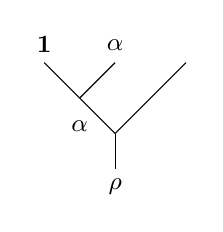
\begin{tikzpicture}[baseline=(current bounding box.center),yscale=0.9,xscale=0.9]
			\draw (0,0.5) -- (0,1);
			\draw (0,1) -- (-0.5,1.5);
			\draw (-0.5,1.5) -- (-1,2);
			\draw (-0.5,1.5) -- (0,2);
			\draw (0,1) -- (0.5,1.5);
			\draw (0.5,1.5) -- (1,2);
			\node at (0,0.25) {\small $\rho$};
			\node at (-1,2.25) {\small $\mathbf{1}$};
			\node at (0,2.25) {\small $\alpha$};
			\node at (1,2.25) {\small $\alphastarrho$};
			\node at (-0.5,1.1) {\small $\alpha$};
		\end{tikzpicture}= \left(F_\rho^{\mathbf{1}\alpha\alphastarrho}\right)_{\rho\alpha}
		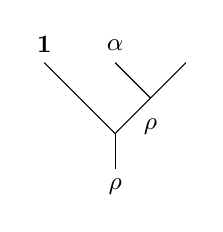
\begin{tikzpicture}[baseline=(current bounding box.center),yscale=0.9,xscale=0.9]
			\draw (0,0.5) -- (0,1);
			\draw (0,1) -- (-0.5,1.5);
			\draw (-0.5,1.5) -- (-1,2);
			\draw (0.5,1.5) -- (0,2);
			\draw (0,1) -- (0.5,1.5);
			\draw (0.5,1.5) -- (1,2);
			\node at (0,0.25) {\small $\rho$};
			\node at (-1,2.25) {\small $\mathbf{1}$};
			\node at (0,2.25) {\small $\alpha$};
			\node at (1,2.25) {\small $\alphastarrho$};
			\node at (0.5,1.1) {\small $\rho$};
		\end{tikzpicture}.
	\end{equation}
According to \cref{eq:tetrahedralsymmetry}, we get the following identities:
	\begin{equation}
		\left(F_\rho^{\mathbf{1}\alpha\alphastarrho}\right)_{\rho\alpha}=\left(F_{\alphastarrho}^{\alpha\mathbf{1}\rho}\right)_{\rho\alpha}=\left(F_\mathbf{1}^{\rho\alphastarrho\alpha}\right)_{\rho\alpha^*}=\left(F_\rho^{\alpha^*\alpha\rho}\right)_{\alphastarrho\mathbf{1}}.
	\end{equation}
However, only the first and the last $F$-symbol coincide (they are both equal to one, see \cref{app:Fsymbols}). The second and third $F$-symbol are not valid: $\left(F_{\alphastarrho}^{\alpha\mathbf{1}\rho}\right)_{\rho\alpha}$ corresponds to a transformation between zero-dimensional vector spaces and $\left(F_\mathbf{1}^{\rho\alphastarrho\alpha}\right)_{\rho\alpha^*}$ has the wrong outer labels, although the vector space is one-dimensional. Due to the different dimensions of the vector spaces, it is not possible to find a gauge transformation that can be applied to the $F$-symbols in order to fulfil the tetrahedral symmetry condition.

Therefore, it has been questioned whether the tetrahedral symmetry condition is necessary for the Levin-Wen model, for example in \cite{Hung2012} and \cite{Lin2014}. The string-net construction in the sense of Levin and Wen is furthermore closely related to so-called Turaev-Viro state sums \cite{Turaev1992a}: It was shown, for example, in \cite{Kadar2010,Koenig2010,Kirillov2011} (and revisited more recently in \cite{Barkeshli2019a,Bauer2019}), that the string-net space of the Levin-Wen construction for a unitary fusion category $\C$ is equal to the state space of a \emph{Turaev-Viro} topological quantum field theory for $\C$. This itself is isomorphic to the state space of the \emph{Reshetikin-Turaev} theory for the Drinfeld double of $\C$, see for example \cite{Kirillov2010,Turaev2010a,Balsam2010}. In both of these theories tetrahedral symmetry does not play any role. While we do not go into detail about these theories here, this observation gives a strong hint that tetrahedral symmetry is not a necessary condition for the construction. In fact, in \cite{Hong2009} it was shown that \emph{any} unitary fusion category yields an exactly solvable Hamiltonian via the string-net construction. 

However, the literature of Turaev-Viro state sums does not provide an explicit way to construct the Hamiltonian from a category the way it was done by Levin and Wen. Especially for physicists who do not necessarily have a solid background in category theory or topology, this lack of a constructive way of defining the Hamiltonian is a serious hurdle when using the Levin-Wen approach for arbitrary UFCs. Therefore, although solved in principle, the construction of the Levin-Wen Hamiltonian without tetrahedral symmetry was still noted as an open problem in the physics literature, for example in \cite{Hung2012}. In \cite{Lin2014}, the authors attacked this problem in the case of fusion categories where the objects form an abelian group under the fusion operation. In \cite{Lan2014}, the authors discuss how to calculate the quasiparticle statistics of the excitations of the model, but do not provide a construction of either the Hamiltonian or the excitations themselves.

Therefore, in the following we describe in detail how the Hamiltonian can be constructed without imposing the tetrahedral symmetry condition on the $F$-symbols, hence making it applicable to all unitary fusion categories.

\section{The Levin-Wen model}

\index{Levin-Wen model}
In their seminal paper \cite{Levin2005}, Levin and Wen explain how topological phases emerge from microscopic degrees of freedom of a physical system. In their string-net model, the universal properties of such a phase are described by the ground state wave function, which is determined from local constraints. The underlying mathematical framework of this theory is that of unitary fusion categories. In the original paper, these categories have to fulfil some additional constraints, among them the tetrahedral symmetry condition introduced in the previous section. In this section we present the basics of the string-net model and explain how the Hamiltonian is constructed. 

As the name suggests, sting-net models are networks of strings of different types\index{string-net}. We focus here on networks that are built from trivalent vertices, which means that at each node exactly three strings meet. However, not all combinations of string types are allowed to meet at a node since the model is restricted by the data of the underlying fusion category. In general, one needs to input the following data to define a string-net model:
	\begin{enumerate}
		\item \textbf{String types.} We need to specify which types of strings (i.e., labels) are allowed in the model. They are given by the simple objects of the underlying category. We usually label different string types with integers: $i=0,1,2,\dots,N$, where $0$ represents the vacuum or unit object\footnote{This notation is different to the category theory language, where we always use $\mathbf{1}$ to indicate the unit object. However, in the string-net literature it is common to use $0$ for the vacuum string.}. The number of simple objects of the category also yields the total number of different string types $N+1$.
		\item \textbf{Branching rules.} It is necessary to specify which string types are allowed to meet at a vertex to identify the allowed string-net configurations:
			\begin{equation}
				\begin{tikzpicture}[scale=0.75,baseline=(current bounding box.center)]
					\draw[->-,>=stealth] (90:1) -- (0,0);
					\draw[->-,>=stealth] (210:1) -- (0,0);
					\draw[->-,>=stealth] (330:1) -- (0,0);
					\node at (90:1.25) {\small $i$};
					\node at (210:1.25) {\small $k$};
					\node at (330:1.25) {\small $j$};
				\end{tikzpicture}.
			\end{equation}
		These rules can be obtained from the fusion rules of the underlying UFC: For instance, the above vertex is an allowed configuration if $N_{kj}^{i^*}>0$. To every string-type $i$ we associate a complex number $d_i$ which is given by the quantum dimension of the simple object in the category.
		\item \textbf{String orientations.} Every string has an arrow to indicate its direction. With every string type $i$ we associate a \emph{dual} string type $i^*$ such that $(i^*)^*=i$. This is possible because a UFC is rigid an therefore has left and right duals. A string of type $i^*$ corresponds to a type-$i$ string with opposite direction:
			\begin{equation}
				\begin{tikzpicture}[baseline=(current bounding box.center)]
					\draw[->-,>=stealth] (0,0) to node[left] {\small $i^*$} (0,-1);
					\draw[->-,>=stealth] (0.5,-1) to node[right] {\small $i$} (0.5,0);
				\end{tikzpicture}.
			\end{equation}
	\end{enumerate}
After specifying this data, defining the Hilbert space of the model is straightforward: The states are given by linear combinations of different  spatial configurations of string-nets.

\begin{rem}
	Before describing the Hamiltonian of the model, some remarks on the graphical notation are in order: 
	\begin{enumerate}
		\item First, we usually use dashed lines to draw a string that corresponds to the vacuum and omit the label $0$:
			\begin{equation}
				\begin{tikzpicture}[baseline={([yshift=-3pt]current bounding box.center)}]
				\draw[dashed] (0,0) -- (0,1);
				\end{tikzpicture}\ \equiv\ 
				\begin{tikzpicture}[baseline={([yshift=-3pt]current bounding box.center)}]
				\draw[->-,>=stealth] (0,0) to node[right] {\small $0$} (0,1);
				\end{tikzpicture}\ .
			\end{equation}
		In this case, it is also not necessary to indicate the direction of the string since the unit object is its own dual.
		\item For clarity we sometimes draw diagrams without indicating the direction of the arrows. In this case, the convention is that all arrows point upwards, for example
			\begin{equation}
				\begin{tikzpicture}[scale=0.75,baseline={([yshift=-3pt]current bounding box.center)}]
				\draw (90:1) -- (0,0);
				\draw (210:1) -- (0,0);
				\draw (330:1) -- (0,0);
				\node at (90:1.25) {\small $i$};
				\node at (210:1.25) {\small $k$};
				\node at (330:1.25) {\small $j$};
				\end{tikzpicture}\equiv 
				\begin{tikzpicture}[scale=0.75,baseline={([yshift=-3pt]current bounding box.center)}]
				\draw[->-,>=stealth] (0,0) -- (90:1);
				\draw[->-,>=stealth] (210:1) -- (0,0);
				\draw[->-,>=stealth] (330:1) -- (0,0);
				\node at (90:1.25) {\small $i$};
				\node at (210:1.25) {\small $k$};
				\node at (330:1.25) {\small $j$};
				\end{tikzpicture}.
			\end{equation}
		\item We use the same normalisation of vertices as discussed in \cref{eq:vertexnorm}. This implies that in graphical calculations we can use the completeness relation \cref{eq:identity} and the bigon relation \cref{eq:bigon2}.
		\item We do not use horizontal lines in the diagrams in this chapter (in contrast to the original paper \cite{Levin2005}). The reason behind this is that the goal of this chapter is to do a construction of the model without imposing tetrahedral symmetry, and without this condition the meaning of horizontal lines is ambiguous. Hence, throughout this chapter we make an effort to translate all diagrams from the original paper to ones without horizontal lines.
	\end{enumerate}	
\end{rem}

In \cite{Levin2005}, the $F$-symbols of the category are required to fulfil several conditions:
	\begin{align}
		\left(F_i^{ijj^*}\right)_{0k}&=\sqrt{\frac{d_k}{d_i d_j}}\ \delta_{ik}^k \label{eq:LWcond1}\\
		\left(F_i^{jkl}\right)_{nm}=\left(F_{l^*}^{kji^*}\right)_{n^*m}&=\left(F_{j^*}^{i^*lk}\right)_{nm^*}=\sqrt{\frac{d_md_n}{d_ld_j}}\left(F_{i^*}^{m^*kn^*}\right)_{l^*j^*} \label{eq:LWcond2}\\
		\left(F_u^{abr}\right)_{sp}\left(F_u^{pcd}\right)_{rq}&=\sum_t \left(F_s^{bcd}\right)_{rt}\left(F_u^{atd}\right)_{sq}\left(F_q^{abc}\right)_{tp} \label{eq:LWcond3}\\
		\overline{\left(F_i^{jkl}\right)}_{nm}&=\left(F_{i^*}^{j^*k^*l^*}\right)_{n^*m^*} \label{eq:LWcond4},
	\end{align}
where  
	\begin{equation}
	\label{eq:delta}
		\delta_{ij}^k=\begin{cases}
		1, & i\otimes j=k \text{ is an allowed fusion}\\
		0, &\mathrm{otherwise.}
		\end{cases}
	\end{equation}
The first one is a normalisation condition similar to the one we derived in \cref{eq:Fidentities}, but a bit more restrictive. The second one is the tetrahedral symmetry condition we derived in \cref{sec:tetrahedral}. The third one is simply the pentagon equation \cref{eq:pentagon}. The last one is a unitarity condition. For the purpose of introducing the Levin-Wen string-net model in this section we assume all of these conditions to be true. In the next section, we explain how to do the construction without imposing all of these conditions\footnote{Note that the pentagon equation always has to be fulfilled since the input category is a unitary fusion category, hence we also require it in the general case.}.

With the definition of the string-net Hilbert space at hand we can write down a Hamiltonian on this space. In general, a string-net Hamiltonian can be any local operator acting on string-net states. The form of this Hamiltonian is determined by certain local relations on its ground state wave function $\Phi$ which arise from scale-invariance, which means the following: We expect that two states within the same topological phase to look the same at long distances. That is, the two wave functions will only differ in short distance details. For instance, at long length scales, a local bubble is irrelevant and will simply look like a string: 
	\begin{equation}
		\Phi\left(
		\begin{tikzpicture}[baseline={([yshift=-3pt]current bounding box.center)}, decoration={markings,mark=at position .55 with {\arrow[>=stealth]{>}}},scale=0.6]
			\draw[{postaction=decorate}] (0.8,0.5) to node[above] {\small $i$} (1.5,0.75);
			\draw[{postaction=decorate}] (1.5,0.75) to [bend right=80] node [below,pos=0.4] {\small $l$} (2.5,1.25);
			\draw[{postaction=decorate}] (1.5,0.75) to [bend left=80] node [above,pos=0.4] {\small $k$} (2.5,1.25);
			\draw[{postaction=decorate}] (2.5,1.25) to node[above] {\small $j$} (3.2,1.5);
			\draw[fill=LightGray,rounded corners,LightGray] (-0.2,0) rectangle (0.8,2);
			\draw[fill=LightGray,rounded corners,LightGray] (3.2,0) rectangle (4.2,2);
		\end{tikzpicture}
		\right) \approx
		\Phi\left(
		\begin{tikzpicture}[baseline={([yshift=-3pt]current bounding box.center)}, decoration={markings,mark=at position .55 with {\arrow[>=stealth]{>}}},scale=0.6]
			\draw[{postaction=decorate}] (0.8,0.5) to node[above] {\small $i$} (2,1);
%			\draw[{postaction=decorate}] (1.5,0.75) to [bend right=80] node [below,pos=0.4] {\small $l$} (2.5,1.25);
%			\draw[{postaction=decorate}] (1.5,0.75) to [bend left=80] node [above,pos=0.4] {\small $k$} (2.5,1.25);
			\draw[{postaction=decorate}] (2,1) to node[above] {\small $j$} (3.2,1.5);
			\node at (2,1) {$\bullet$};
			\draw[fill=LightGray,rounded corners,LightGray] (-0.2,0) rectangle (0.8,2);
			\draw[fill=LightGray,rounded corners,LightGray] (3.2,0) rectangle (4.2,2);
		\end{tikzpicture}
		\right)
	\end{equation}
However, if $i\neq j$, the configuration on the right hand side is invalid, which yields
	\begin{equation}
		\Phi\left(
		\begin{tikzpicture}[baseline={([yshift=-3pt]current bounding box.center)}, decoration={markings,mark=at position .55 with {\arrow[>=stealth]{>}}},scale=0.6]
			\draw[{postaction=decorate}] (0.8,0.5) to node[above] {\small $i$} (2,1);
			%			\draw[{postaction=decorate}] (1.5,0.75) to [bend right=80] node [below,pos=0.4] {\small $l$} (2.5,1.25);
			%			\draw[{postaction=decorate}] (1.5,0.75) to [bend left=80] node [above,pos=0.4] {\small $k$} (2.5,1.25);
			\draw[{postaction=decorate}] (2,1) to node[above] {\small $j$} (3.2,1.5);
			\node at (2,1) {$\bullet$};
			\draw[fill=LightGray,rounded corners,LightGray] (-0.2,0) rectangle (0.8,2);
			\draw[fill=LightGray,rounded corners,LightGray] (3.2,0) rectangle (4.2,2);
		\end{tikzpicture}
		\right)=0.
	\end{equation}
As a result, we conclude that the amplitude vanishes if $i\neq j$. Similar considerations yield the following set of local relations: 
	\begin{align}
		\Phi\left(
		\begin{tikzpicture}[baseline={([yshift=-3pt]current bounding box.center)}, decoration={markings,mark=at position .5 with {\arrow[>=stealth]{>}}},scale=0.6]
		\draw[{postaction=decorate}] (1,0.5) to node[above] {\small $i$} (3,1.5);
		\draw[fill=LightGray,rounded corners,LightGray] (0,0) rectangle (1,2);
		\draw[fill=LightGray,rounded corners,LightGray] (3,0) rectangle (4,2);
		\end{tikzpicture}\right)
		&=	\Phi\left(	
		\begin{tikzpicture}[baseline={([yshift=-3pt]current bounding box.center)}, decoration={markings,mark=at position .5 with {\arrow[>=stealth]{>}}},scale=0.6]
		\draw[{postaction=decorate}] (1,0.5) -- (1.5,0.75) to [bend right=80] node [above,pos=0.4] {\small $i$} (2.5,1.25) -- (3,1.5);
		\draw[fill=LightGray,rounded corners,LightGray] (0,0) rectangle (1,2);
		\draw[fill=LightGray,rounded corners,LightGray] (3,0) rectangle (4,2);
		\end{tikzpicture}\right) \label{eq:groundstate1}\\
		\Phi\left(
		\begin{tikzpicture}[baseline={([yshift=-3pt]current bounding box.center)}, decoration={markings,mark=at position .0 with {\arrow[>=stealth]{>}}},scale=0.6]
		\draw[fill=LightGray,rounded corners,LightGray] (0,0) rectangle (1,2);
		\draw[{postaction=decorate}] (2,1) circle (0.5cm);
		\node at (2.9,1) {\small $i$};
		\end{tikzpicture}
		\right)	
		&=d_i \ \Phi\left(
		\begin{tikzpicture}[baseline={([yshift=-3pt]current bounding box.center)}, decoration={markings,mark=at position .0 with {\arrow[>=stealth]{>}}},scale=0.6]
		\draw[fill=LightGray,rounded corners,LightGray] (0,0) rectangle (1,2);
		\end{tikzpicture}
		\right) \label{eq:groundstate2}\\
		\Phi\left(
		\begin{tikzpicture}[baseline={([yshift=-3pt]current bounding box.center)}, decoration={markings,mark=at position .55 with {\arrow[>=stealth]{>}}},scale=0.6]
		\draw[{postaction=decorate}] (0.8,0.5) to node[above] {\small $i$} (1.5,0.75);
		\draw[{postaction=decorate}] (1.5,0.75) to [bend right=80] node [below,pos=0.4] {\small $l$} (2.5,1.25);
		\draw[{postaction=decorate}] (1.5,0.75) to [bend left=80] node [above,pos=0.4] {\small $k$} (2.5,1.25);
		\draw[{postaction=decorate}] (2.5,1.25) to node[above] {\small $j$} (3.2,1.5);
		\draw[fill=LightGray,rounded corners,LightGray] (-0.2,0) rectangle (0.8,2);
		\draw[fill=LightGray,rounded corners,LightGray] (3.2,0) rectangle (4.2,2);
		\end{tikzpicture}
		\right) 
		&=\delta_{ij}\ \Phi\left(
		\begin{tikzpicture}[baseline={([yshift=-3pt]current bounding box.center)}, decoration={markings,mark=at position .6 with {\arrow[>=stealth]{>}}},scale=0.6]
		\draw[{postaction=decorate}] (0.8,0.5) to node[above] {\small $i$} (1.5,0.75);
		\draw[{postaction=decorate}] (1.5,0.75) to [bend right=80] node [below,pos=0.4] {\small $l$} (2.5,1.25);
		\draw[{postaction=decorate}] (1.5,0.75) to [bend left=80] node [above,pos=0.4] {\small $k$} (2.5,1.25);
		\draw[{postaction=decorate}] (2.5,1.25) to node[above] {\small $i$} (3.2,1.5);
		\draw[fill=LightGray,rounded corners,LightGray] (-0.2,0) rectangle (0.8,2);
		\draw[fill=LightGray,rounded corners,LightGray] (3.2,0) rectangle (4.2,2);
		\end{tikzpicture}
		\right) \label{eq:groundstate3}\\
		\Phi\left(
		\begin{tikzpicture}[baseline={([yshift=-3pt]current bounding box.center)}, decoration={markings,mark=at position .6 with {\arrow[>=stealth]{>}}},scale=0.6]
		\draw[fill=LightGray,rounded corners,LightGray] (0,-0.2) rectangle (2,0.8);
		\draw[fill=LightGray,rounded corners,LightGray] (0,3.2) rectangle (2,4.2);
		\draw[{postaction=decorate}] (0.5,0.8) to node[left] {\small $i$} (0.5,2.5);
		\draw[{postaction=decorate}] (0.5,2.5) to node[left] {\small $k$} (0.5,3.2);
		\draw[{postaction=decorate}] (1.5,0.8) to node[right] {\small $j$} (1.5,1.5);
		\draw[{postaction=decorate}] (1.5,1.5) to node[right] {\small $l$} (1.5,3.2);
		\draw[{postaction=decorate}] (1.5,1.5) to node[above] {\small $m$} (0.5,2.5);
		\end{tikzpicture}\right) &=\sum_n \left(G_{ij}^{kl}\right)_{nm}\ \Phi\left(
		\begin{tikzpicture}[baseline={([yshift=-3pt]current bounding box.center)}, decoration={markings,mark=at position .6 with {\arrow[>=stealth]{>}}},scale=0.6]
		\draw[fill=LightGray,rounded corners,LightGray] (0,-0.2) rectangle (2,0.8);
		\draw[fill=LightGray,rounded corners,LightGray] (0,3.2) rectangle (2,4.2);
		\draw[{postaction=decorate}] (0.5,0.8) to node[left] {\small $i$} (1,1.5);
		\draw[{postaction=decorate}] (1.5,0.8) to node[right] {\small $j\ $} (1,1.5);
		\draw[{postaction=decorate}] (1,1.5) to node[right] {\small $n$} (1,2.5);
		\draw[{postaction=decorate}] (1,2.5) to node[left] {\small $\ k$} (0.5,3.2);
		\draw[{postaction=decorate}] (1,2.5) to node[right] {\small $l$} (1.5,3.2);
		\end{tikzpicture}
		\right) \label{eq:groundstate4}\\
		\Phi\left(
		\begin{tikzpicture}[baseline={([yshift=-3pt]current bounding box.center)}, decoration={markings,mark=at position .6 with {\arrow[>=stealth]{>}}},scale=0.6]
		\draw[fill=LightGray,rounded corners,LightGray] (0,-0.2) rectangle (2,0.8);
		\draw[fill=LightGray,rounded corners,LightGray] (0,3.2) rectangle (2,4.2);
		\draw[{postaction=decorate}] (0.5,0.8) to node[left] {\small $i$} (0.5,1.5);
		\draw[{postaction=decorate}] (0.5,1.5) to node[left] {\small $k$} (0.5,3.2);
		\draw[{postaction=decorate}] (1.5,0.8) to node[right] {\small $j$} (1.5,2.5);
		\draw[{postaction=decorate}] (1.5,2.5) to node[right] {\small $l$} (1.5,3.2);
		\draw[{postaction=decorate}] (0.5,1.5) to node[above] {\small $m$} (1.5,2.5);
		\end{tikzpicture}\right) &=\sum_n \left(H_{ij}^{kl}\right)_{nm}\ \Phi\left(
		\begin{tikzpicture}[baseline={([yshift=-3pt]current bounding box.center)}, decoration={markings,mark=at position .6 with {\arrow[>=stealth]{>}}},scale=0.6]
		\draw[fill=LightGray,rounded corners,LightGray] (0,-0.2) rectangle (2,0.8);
		\draw[fill=LightGray,rounded corners,LightGray] (0,3.2) rectangle (2,4.2);
		\draw[{postaction=decorate}] (0.5,0.8) to node[left] {\small $i$} (1,1.5);
		\draw[{postaction=decorate}] (1.5,0.8) to node[right] {\small $j\ $} (1,1.5);
		\draw[{postaction=decorate}] (1,1.5) to node[right] {\small $n$} (1,2.5);
		\draw[{postaction=decorate}] (1,2.5) to node[left] {\small $\ k$} (0.5,3.2);
		\draw[{postaction=decorate}] (1,2.5) to node[right] {\small $l$} (1.5,3.2);
		\end{tikzpicture}
		\right). \label{eq:groundstate5}
	\end{align}
The grey rectangles represent the remaining parts of the string-net configuration that is left unchanged by the local relations. Note that we have slightly changed the relation in contrast to the original formulation to avoid horizontal lines. In \cite{Levin2005}, the relations \cref{eq:groundstate4} and \cref{eq:groundstate5} are summarized as
	\begin{equation}
	\label{eq:normalcond}
		\Phi\left(
		\begin{tikzpicture}[baseline={([yshift=-3pt]current bounding box.center)}, decoration={markings,mark=at position .6 with {\arrow[>=stealth]{>}}},scale=0.6]
		\draw[{postaction=decorate}] (0.8,0.5) to node[below] {\small $j$} (1.5,1);
		\draw[{postaction=decorate}] (0.8,1.5) to node[above] {\small $i$} (1.5,1);
		\draw[{postaction=decorate}] (3.2,0.5) to node[below] {\small $k$} (2.5,1);
		\draw[{postaction=decorate}] (3.2,1.5) to node[above] {\small $l$} (2.5,1);
		\draw[{postaction=decorate}] (2.5,1) to node[above] {\small $m$} (1.5,1);
		\draw[fill=LightGray,rounded corners,LightGray] (-0.2,0) rectangle (0.8,2);
		\draw[fill=LightGray,rounded corners,LightGray] (3.2,0) rectangle (4.2,2);
		\end{tikzpicture}\right) 
		=\sum_n \left(F_k^{j^*i^*l^*}\right)_{nm}\ \Phi\left(
		\begin{tikzpicture}[baseline={([yshift=-3pt]current bounding box.center)}, decoration={markings,mark=at position .6 with {\arrow[>=stealth]{>}}},scale=0.6]
		\draw[{postaction=decorate}] (0.8,0.5) to node[below] {\small $j$} (2,0.5);
		\draw[{postaction=decorate}] (3.2,0.5) to node[below] {\small $k$} (2,0.5);
		\draw[{postaction=decorate}] (0.8,1.5) to node[above] {\small $i$} (2,1.5);
		\draw[{postaction=decorate}] (3.2,1.5) to node[above] {\small $l$} (2,1.5);
		\draw[{postaction=decorate}] (2,0.5) to node[right] {\small $n$} (2,1.5);
		\draw[fill=LightGray,rounded corners,LightGray] (-0.2,0) rectangle (0.8,2);
		\draw[fill=LightGray,rounded corners,LightGray] (3.2,0) rectangle (4.2,2);
		\end{tikzpicture}
		\right).
	\end{equation}
The operators $G$ and $H$ in \cref{eq:groundstate4} and \cref{eq:groundstate5} are related to the $F$-symbols of the underlying fusion category. They are computed by applying the completeness relation \cref{eq:identity} to the diagrams on both sides. For instance, the computation of $H$ works as follows:
	\begin{align}
		\begin{tikzpicture}[scale=0.8,decoration={markings,mark=at position .55 with {\arrow[>=stealth]{>}}},baseline=(current bounding box.center)]
		\node (a) at (0,-0.25) {\small $i$};
		\node (c) at (0,2.25) {\small $k$};
		\node (b) at (1,-0.25) {\small $j$};
		\node (d) at (1,2.25) {\small $l$};
		\draw[{postaction=decorate}] (0,0) -- (0,0.6);
		\draw[{postaction=decorate}] (0,0.6) -- (0,2);
		\draw[{postaction=decorate}] (1,0) -- (1,1.4);
		\draw[{postaction=decorate}] (1,1.4) -- (1,2);
		\draw[{postaction=decorate}] (0,0.6) -- node[above] {\small $m$} (1,1.4);
		\end{tikzpicture}
		&= \sum_n \sqrt{\frac{d_n}{d_i d_j}}\ 
		\begin{tikzpicture}[scale=0.8,decoration={markings,mark=at position .55 with {\arrow[>=stealth]{>}}},baseline=(current bounding box.center)]
		\node (a) at (-0.25,0.1) {\small $i$};
		\node (c) at (0,2) {\small $k$};
		\node (b) at (1.25,0.1) {\small $j$};
		\node (d) at (1,2) {\small $l$};
		\draw[{postaction=decorate}] (0,0.6) -- (0,1.75);
		\draw[{postaction=decorate}] (0.5,-0.25) -- (1,0.25);
		\draw (1,0.25) -- (1,1.4);
		\draw[{postaction=decorate}] (1,1.4) -- (1,1.75);
		\draw[{postaction=decorate}] (0,0.6) -- node[above] {\small $m$} (1,1.4);
		\draw[{postaction=decorate}] (0.5,-0.25) -- (0,0.25);
		\draw (0,0.25) -- (0,0.6);
		\draw[{postaction=decorate}] (0.5,-0.75) to node[right] {\small $n$} (0.5,-0.25);
		\draw[{postaction=decorate}] (0,-1.25) -- (0.5,-0.75);
		\draw[{postaction=decorate}] (1,-1.25) -- (0.5,-0.75);
		\node at (-0.25,-1.25) {\small $i$};
		\node at (1.25,-1.25) {\small $j$};
		\end{tikzpicture}\\
		&=\sum_{n,\alpha} \sqrt{\frac{d_n}{d_i d_j}} \left(F_n^{kmj}\right)_{\alpha i}
		\begin{tikzpicture}[scale=0.8,decoration={markings,mark=at position .61 with {\arrow[>=stealth]{>}}},baseline=(current bounding box.center)]
		\node (a) at (-0.25,0.1) {\small $i$};
		\node (c) at (0,2) {\small $k$};
		\node (b) at (1.25,0.1) {\small $\alpha$};
		\node (d) at (1,2) {\small $l$};
		\draw[{postaction=decorate}] (0,0.6) -- (0,1.75);
		\draw[{postaction=decorate}] (0.5,-0.25) -- (1,0.25);
		\draw (1,0.25) -- (1,0.6);
		\draw[{postaction=decorate}] (1,1.4) -- (1,1.75);
		\draw[{postaction=decorate}] (1,1.4) -- (1,1.75);
		\draw[{postaction=decorate}] (1,0.6) -- (0.6,1);
		\draw (0.6,1) -- (1,1.4);
		\draw[{postaction=decorate}] (1,0.6) -- (1.4,1);
		\draw (1.4,1) -- (1,1.4);
		\draw[{postaction=decorate}] (0.5,-0.25) -- (0,0.25);
		\draw (0,0.25) -- (0,0.6);
		\draw[{postaction=decorate}] (0.5,-0.75) to node[right] {\small $n$} (0.5,-0.25);
		\draw[{postaction=decorate}] (0,-1.25) -- (0.5,-0.75);
		\draw[{postaction=decorate}] (1,-1.25) -- (0.5,-0.75);
		\node at (-0.25,-1.25) {\small $i$};
		\node at (1.25,-1.25) {\small $j$};
		\node at (1.6,1) {\small $j$};
		\node at (0.4,1) {\small $m$};
		\end{tikzpicture}\\
		&=\sum_{n,\alpha} \sqrt{\frac{d_n}{d_i d_j}} \left(F_n^{kmj}\right)_{\alpha i}\sqrt{\frac{d_m d_j}{d_l}}\  \delta_{l,\alpha}
		\begin{tikzpicture}[scale=0.8,decoration={markings,mark=at position .5 with {\arrow[>=stealth]{>}}},baseline=(current bounding box.center)]
		\draw[{postaction=decorate}] (0.5,-0.25) -- (0,0.25);
		\draw[{postaction=decorate}] (0.5,-0.25) -- (1,0.25);
		\draw[{postaction=decorate}] (0.5,-0.75) to node[right] {\small $n$} (0.5,-0.25);
		\draw[{postaction=decorate}] (0,-1.25) -- (0.5,-0.75);
		\draw[{postaction=decorate}] (1,-1.25) -- (0.5,-0.75);
		\node at (0,-1.5) {\small $i$};
		\node at (1,-1.5) {\small $j$};
		\node at (0,0.5) {\small $k$};
		\node at (1,0.5) {\small $l$};
		\end{tikzpicture}\\
		&=\sum_n \sqrt{\frac{d_m d_n}{d_i d_l}} \left(F_n^{kmj}\right)_{li}
		\begin{tikzpicture}[scale=0.8,decoration={markings,mark=at position .5 with {\arrow[>=stealth]{>}}},baseline=(current bounding box.center)]
		\draw[{postaction=decorate}] (0.5,-0.25) -- (0,0.25);
		\draw[{postaction=decorate}] (0.5,-0.25) -- (1,0.25);
		\draw[{postaction=decorate}] (0.5,-0.75) to node[right] {\small $n$} (0.5,-0.25);
		\draw[{postaction=decorate}] (0,-1.25) -- (0.5,-0.75);
		\draw[{postaction=decorate}] (1,-1.25) -- (0.5,-0.75);
		\node at (0,-1.5) {\small $i$};
		\node at (1,-1.5) {\small $j$};
		\node at (0,0.5) {\small $k$};
		\node at (1,0.5) {\small $l$};
		\end{tikzpicture},
	\end{align}
which yields
	\begin{equation}
	\label{eq:Hop}
		\left(H_{ij}^{kl}\right)_{nm}=\sqrt{\frac{d_m d_n}{d_i d_l}}\left(F_n^{kmj}\right)_{li}.
	\end{equation}
A similar calculation for $G$ yields
	\begin{equation}
	\label{eq:Gop}
		\left(G_{ij}^{kl}\right)_{nm}=\sqrt{\frac{d_m d_n}{d_j d_k}}\overline{\left(F_n^{iml}\right)}_{kj}.
	\end{equation}
Note that imposing tetrahedral symmetry on the $F$-symbols implies that the vertices in \cref{eq:groundstate4} and \cref{eq:groundstate5} can be moved up and down arbitrarily, i.e.
	\begin{equation}
		\begin{tikzpicture}[baseline={([yshift=-3pt]current bounding box.center)}, decoration={markings,mark=at position .6 with {\arrow[>=stealth]{>}}},scale=0.6]
			\draw[fill=LightGray,rounded corners,LightGray] (0,-0.2) rectangle (2,0.8);
			\draw[fill=LightGray,rounded corners,LightGray] (0,3.2) rectangle (2,4.2);
			\draw[{postaction=decorate}] (0.5,0.8) to node[left] {\small $i$} (0.5,2.5);
			\draw[{postaction=decorate}] (0.5,2.5) to node[left] {\small $k$} (0.5,3.2);
			\draw[{postaction=decorate}] (1.5,0.8) to node[right] {\small $j$} (1.5,1.5);
			\draw[{postaction=decorate}] (1.5,1.5) to node[right] {\small $l$} (1.5,3.2);
			\draw[{postaction=decorate}] (1.5,1.5) to node[above] {\small $m$} (0.5,2.5);
		\end{tikzpicture}=\begin{tikzpicture}[baseline={([yshift=-3pt]current bounding box.center)}, decoration={markings,mark=at position .6 with {\arrow[>=stealth]{>}}},scale=0.6]
			\draw[fill=LightGray,rounded corners,LightGray] (0,-0.2) rectangle (2,0.8);
			\draw[fill=LightGray,rounded corners,LightGray] (0,3.2) rectangle (2,4.2);
			\draw[{postaction=decorate}] (0.5,0.8) to node[left] {\small $i$} (0.5,1.5);
			\draw[{postaction=decorate}] (0.5,1.5) to node[left] {\small $k$} (0.5,3.2);
			\draw[{postaction=decorate}] (1.5,0.8) to node[right] {\small $j$} (1.5,2.5);
			\draw[{postaction=decorate}] (1.5,2.5) to node[right] {\small $l$} (1.5,3.2);
			\draw[{postaction=decorate}] (1.5,2.5) to node[above] {\small $m$} (0.5,1.5);
		\end{tikzpicture}\equiv
		\begin{tikzpicture}[baseline={([yshift=-3pt]current bounding box.center)}, decoration={markings,mark=at position .6 with {\arrow[>=stealth]{>}}},scale=0.6]
			\draw[fill=LightGray,rounded corners,LightGray] (0,-0.2) rectangle (2,0.8);
			\draw[fill=LightGray,rounded corners,LightGray] (0,3.2) rectangle (2,4.2);
			\draw[{postaction=decorate}] (0.5,0.8) to node[left] {\small $i$} (0.5,2);
			\draw[{postaction=decorate}] (0.5,2) to node[left] {\small $k$} (0.5,3.2);
			\draw[{postaction=decorate}] (1.5,0.8) to node[right] {\small $j$} (1.5,2);
			\draw[{postaction=decorate}] (1.5,2) to node[right] {\small $l$} (1.5,3.2);
			\draw[{postaction=decorate}] (1.5,2) to node[above] {\small $m$} (0.5,2);
		\end{tikzpicture}.
	\end{equation}
This can also be seen by manipulating the operators $G$ and $H$ using the conditions listed in \cref{eq:LWcond1,eq:LWcond2,eq:LWcond3,eq:LWcond4}:
	\begin{align}
		\left(G_{ij}^{kl}\right)_{nm}&=\sqrt{\frac{d_m d_n}{d_j d_k}}\overline{\left(F_n^{iml}\right)}_{kj}\\
		&=\sqrt{\frac{d_m d_n}{d_j d_k}}\left(F_{n^*}^{i^*m^*l^*}\right)_{k^*j^*}\\
		&=\sqrt{\frac{d_m d_n}{d_j d_k}}\sqrt{\frac{d_j d_k}{d_l d_i}}\left(F_n^{km^* j}\right)_{li}\\
		&=\left(H_{ij}^{kl}\right)_{nm^*}.
	\end{align}
Hence, if we impose tetrahedral symmetry on the $F$-symbols, the operators $G$ and $H$ are equal. Moreover, the conditions \cref{eq:groundstate4} and \cref{eq:groundstate5} are then equal to the original relation \cref{eq:normalcond} in the form
	\begin{equation}
		\Phi\left(
		\begin{tikzpicture}[baseline={([yshift=-3pt]current bounding box.center)}, decoration={markings,mark=at position .6 with {\arrow[>=stealth]{>}}},scale=0.6]
		\draw[{postaction=decorate}] (0.8,0.5) to node[below] {\small $i$} (1.5,1);
		\draw[{postaction=decorate}] (1.5,1) to node[above] {\small $k$} (0.8,1.5);
		\draw[{postaction=decorate}] (3.2,0.5) to node[below] {\small $j$} (2.5,1);
		\draw[{postaction=decorate}] (2.5,1) to node[above] {\small $l$} (3.2,1.5);
		\draw[{postaction=decorate}] (2.5,1) to node[above] {\small $m$} (1.5,1);
		\draw[fill=LightGray,rounded corners,LightGray] (-0.2,0) rectangle (0.8,2);
		\draw[fill=LightGray,rounded corners,LightGray] (3.2,0) rectangle (4.2,2);
		\end{tikzpicture}\right) 
		=\sum_n \left(F_j^{i^*kl}\right)_{nm}\ \Phi\left(
		\begin{tikzpicture}[baseline={([yshift=-3pt]current bounding box.center)}, decoration={markings,mark=at position .6 with {\arrow[>=stealth]{>}}},scale=0.6]
		\draw[{postaction=decorate}] (0.8,0.5) to node[below] {\small $i$} (2,0.5);
		\draw[{postaction=decorate}] (3.2,0.5) to node[below] {\small $j$} (2,0.5);
		\draw[{postaction=decorate}] (2,1.5) to node[above] {\small $k$} (0.8,1.5);
		\draw[{postaction=decorate}] (2,1.5) to node[above] {\small $l$} (3.2,1.5);
		\draw[{postaction=decorate}] (2,0.5) to node[right] {\small $n$} (2,1.5);
		\draw[fill=LightGray,rounded corners,LightGray] (-0.2,0) rectangle (0.8,2);
		\draw[fill=LightGray,rounded corners,LightGray] (3.2,0) rectangle (4.2,2);
		\end{tikzpicture}
		\right).,
	\end{equation}
which can be seen by applying the tetrahedral symmetry condition \cref{eq:LWcond2} twice:
	\begin{align}
		\left(F_j^{i^*kl}\right)_{nm}&=\sqrt{\frac{d_m d_n}{d_l d_i}}\left(F_{j^*}^{m* k n^*}\right)_{l^* i}\\
		&=\sqrt{\frac{d_m d_n}{d_l d_i}} \left(F_n^{km^* j}\right)_{li}\\
		&=\left(H_{ij}^{kl}\right)_{nm^*}.
	\end{align}
As a result, we can say that the conditions \cref{eq:groundstate4} and \cref{eq:groundstate5} are indeed a true generalization of the original condition \cref{eq:normalcond} by Levin and Wen and replacing their condition does not have an effect on the model in case we assume tetrahedral symmetry.

After having specified the local constraints that uniquely specify the ground state we can construct the exactly solvable lattice Hamiltonian that has exactly these states as ground states. We concentrate here on the honeycomb lattice where the degrees of freedom are on the edges, which goes well with the constraint of using only trivalent vertices. The Hamiltonian consists of two types of operators: ones that act on vertices $\mathbf{v}$ and ones that act on plaquettes $\mathbf{p}$. 

The vertex operators\index{vertex operator} (also called \emph{electric charge operators}\index{electric charge operator}) are denoted $Q_\mathbf{v}$. They always act on three degrees of freedom that meet at a vertex (see \cref{fig:honeycomb}) and they ensure that the ground state of the Hamiltonian only consists of configurations that are allowed by the branching rules:
	\begin{equation}
		Q_\mathbf{v}\Bigg|\begin{tikzpicture}[baseline=(current bounding box.center), decoration={markings,mark=at position .5 with {\arrow[>=stealth]{>}}},scale=0.5]
		\draw[{postaction=decorate}] (330:1cm) to node[below] {\small $j$} (0,0);
		\draw[{postaction=decorate}] (210:1cm) to node[below] {\small $i$} (0,0);
		\draw[{postaction=decorate}] (90:1cm) to node[right] {\small $k$} (0,0);
		\end{tikzpicture}\Bigg\rangle=\delta_{ij}^{k^*}
		\Bigg|\begin{tikzpicture}[baseline=(current bounding box.center), decoration={markings,mark=at position .5 with {\arrow[>=stealth]{>}}},scale=0.5]
		\draw[{postaction=decorate}] (330:1cm) to node[below] {\small $j$} (0,0);
		\draw[{postaction=decorate}] (210:1cm) to node[below] {\small $i$} (0,0);
		\draw[{postaction=decorate}] (90:1cm) to node[right] {\small $k$} (0,0);
		\end{tikzpicture}\Bigg\rangle,
	\end{equation}
with $\delta_{ij}^k$ defined in \cref{eq:delta}.	
	
\begin{figure}[t]
	\centering
		\begin{tikzpicture}[scale=0.8]
		\clip(-4,-1.5) rectangle (6.5,4.5);
		\begin{scope}
		\rotatebox{30}{
			\draw[gray] (0:1cm) -- (60:1cm) -- (120:1cm) -- (180:1cm) -- (240:1cm) -- (300:1cm) -- (0:1cm);
			\draw[LinkColor,thick] (60:1cm) -- (120:1cm) -- (180:1cm);
			\node at (-0.25,1.25) {\rotatebox{-30}{$\mathbf{v}$}};
			\begin{scope}[xshift=0,yshift=1.74cm]
			\draw[gray] (300:1cm) -- (0:1cm) -- (60:1cm) -- (120:1cm) -- (180:1cm) -- (240:1cm);
			\draw[LinkColor,thick] (180:1cm) -- (240:1cm);
			\end{scope}
			\begin{scope}[xshift=1.5cm,yshift=0.87cm]
			\draw[gray]  (240:1cm) -- (300:1cm) -- (0:1cm) -- (60:1cm) -- (120:1cm);
			\draw[LinkColor,thick] (240:1cm) -- (300:1cm);%external leg
			\draw[LinkColor,thick] (0:1cm) -- (60:1cm);%external leg
			\end{scope}
			\begin{scope}[xshift=-1.5cm,yshift=0.87cm]
			\draw[gray] (60:1cm) -- (120:1cm) -- (180:1cm) -- (240:1cm) -- (300:1cm);
			\end{scope}
			\begin{scope}[xshift=-1.5cm,yshift=2.61cm]
			\draw[gray] (0:1cm) -- (60:1cm) -- (120:1cm) -- (180:1cm) -- (240:1cm);
			\end{scope}
			\begin{scope}[xshift=3cm,yshift=-1.74cm]
			\draw[gray] (180:1cm) -- (240:1cm) -- (300:1cm) -- (0:1cm);
			\end{scope}
			\begin{scope}[xshift=1.5cm,yshift=-0.87cm]
			\draw[gray] (180:1cm) -- (240:1cm) -- (300:1cm) -- (0:1cm) -- (60:1cm);
			\draw[LinkColor,thick] (300:1cm) -- (0:1cm);%external leg
			\end{scope}
			\begin{scope}[xshift=3cm,yshift=0cm]
			\draw[thick,LinkColor,fill=LightGray] (240:1cm) -- (300:1cm)-- (0:1cm) -- (60:1cm) -- (120:1cm) -- (120:1cm) -- (180:1cm) -- cycle;
			\node at (0,0) {\rotatebox{-30}{$\mathbf{p}$}};
			\end{scope}
			\begin{scope}[xshift=3cm,yshift=1.74cm]
			\draw[gray] (300:1cm) -- (0:1cm) -- (60:1cm) -- (120:1cm) -- (180:1cm);
			\draw[thick,LinkColor] (300:1cm) -- (0:1cm);%external leg
			\end{scope}
			\begin{scope}[xshift=1.5cm,yshift=2.61cm]
			\draw[gray] (0:1cm) -- (60:1cm) -- (120:1cm) -- (180:1cm);
			\end{scope}
			\begin{scope}[xshift=0,yshift=3.48cm]
			\draw[gray] (0:1cm) -- (60:1cm) -- (120:1cm) -- (180:1cm);
			\end{scope}
			\begin{scope}[xshift=6cm,yshift=0cm]
			\draw[gray] (240:1cm) -- (300:1cm) -- (0:1cm) -- (60:1cm) -- (120:1cm);
			\end{scope}
			\begin{scope}[xshift=4.5cm,yshift=-2.61cm]
			\draw[gray] (180:1cm) -- (240:1cm) -- (300:1cm) -- (0:1cm) -- (60:1cm);
			\end{scope}
			\begin{scope}[xshift=4.5cm,yshift=0.87cm]
			\draw[gray] (240:1cm) -- (300:1cm) -- (0:1cm) -- (60:1cm) -- (120:1cm);
			\draw[LinkColor,thick] (240:1cm) -- (300:1cm);%external leg
			\end{scope}
			\begin{scope}[xshift=4.5cm,yshift=-0.87cm]
			\draw[gray] (180:1cm) -- (240:1cm) -- (300:1cm) -- (0:1cm) -- (60:1cm);
			\draw[LinkColor,thick] (180:1cm) -- (240:1cm);%external leg
			\end{scope}}
		\end{scope}
		\end{tikzpicture}
	\caption{\small \textbf{Hamiltonian on the honeycomb lattice.} A general Hamiltonian consists of operators that act on vertices $Q_\mathbf{v}$ and ones that act on plaquettes $B_\mathbf{p}$.\label{fig:honeycomb}}
\end{figure}

The plaquette operator\index{plaquette operator} $B_\mathbf{p}$ (also called \emph{magnetic flux operator}\index{magnetic flux operator}) imposes dynamics to the system. It acts on all twelve degrees of freedom of a plaquette (see \cref{fig:honeycomb}). It is a linear combination of $N+1$ terms, one term for each string type:
	\begin{equation}
		B_\mathbf{p}=\sum_{s=0}^N a_s B_\mathbf{p}^s,
	\end{equation}
with $a_s=\frac{d_s}{D^2}$, where $D^2=\sum_{i=0}^N d_i^2$ is the total quantum dimension\footnote{In general, the coefficients $a_s$ only have to fulfil the condition $a_{s^*}=a_s^*$ but are otherwise arbitrary. However, the authors of \cite{Levin2005} find that the choice we make here corresponds to a smooth continuum limit where the ground state is topologically invariant. Furthermore, this choice is a requirement for the operators $Q_\mathbf{v}$ and $B_\mathbf{p}$ to be projection operators, hence we adapt it here.}. Each ot the individual terms $B_\mathbf{p}^s$ acts on the plaquette $\mathbf{p}$ by inserting a loop of string type $s$ and fusing this loop into the internal links of the plaquette. Hence, the operator only changes the configuration of internal edges from $g,h,i,j,k,l$ to $g',h',i',j',k',l'$ but leaves the outer strings unchanged: 
	\begin{equation}
	\label{eq:Bcoeff}
		B_\mathbf{p}^s\ \Bigg|\begin{tikzpicture}[baseline={([yshift=-3pt]current bounding box.center)},scale=1.1]
		\draw[->-,>=stealth] (90:0.75) to node[above] {\small $g$} (150:0.75);
		\draw[->-,>=stealth] (150:0.75) to node[left] {\small $l$} (210:0.75);
		\draw[->-,>=stealth] (210:0.75) to node[below] {\small $k$} (270:0.75);
		\draw[->-,>=stealth] (270:0.75) to node[below] {\small $j$} (330:0.75);
		\draw[->-,>=stealth] (330:0.75) to node[right] {\small $i$} (30:0.75);
		\draw[->-,>=stealth] (30:0.75) to node[above] {\small $h$} (90:0.75);
		\foreach \a in {30,90,...,330}{
			\draw[->-,>=stealth] (\a:1) -- (\a:0.75);	
		}
		\node at (90:1.15) {\small $b$};
		\node at (150:1.15) {\small $a$};
		\node at (210:1.15) {\small $f$};
		\node at (270:1.15) {\small $e$};
		\node at (330:1.15) {\small $d$};
		\node at (30:1.15) {\small $c$};
		\end{tikzpicture}\Bigg\rangle=\Bigg|
		\begin{tikzpicture}[baseline={([yshift=-3pt]current bounding box.center)},scale=1.1]
		\draw[->-,>=stealth] (90:0.5) -- (150:0.5);
		\draw[->-,>=stealth] (150:0.5) to node[right] {\small $s$} (210:0.5);
		\draw[->-,>=stealth] (210:0.5) -- (270:0.5);
		\draw[->-,>=stealth] (270:0.5) -- (330:0.5);
		\draw[->-,>=stealth] (330:0.5) to node[left] {\small $s$} (30:0.5);
		\draw[->-,>=stealth] (30:0.5) -- (90:0.5);
		\draw[->-,>=stealth] (90:0.75) to node[above] {\small $g$} (150:0.75);
		\draw[->-,>=stealth] (150:0.75) to node[left] {\small $l$} (210:0.75);
		\draw[->-,>=stealth] (210:0.75) to node[below] {\small $k$} (270:0.75);
		\draw[->-,>=stealth] (270:0.75) to node[below] {\small $j$} (330:0.75);
		\draw[->-,>=stealth] (330:0.75) to node[right] {\small $i$} (30:0.75);
		\draw[->-,>=stealth] (30:0.75) to node[above] {\small $h$} (90:0.75);
		\foreach \a in {30,90,...,330}{
			\draw[->-,>=stealth] (\a:1) -- (\a:0.75);	
		}
		\node at (90:1.15) {\small $b$};
		\node at (150:1.15) {\small $a$};
		\node at (210:1.15) {\small $f$};
		\node at (270:1.15) {\small $e$};
		\node at (330:1.15) {\small $d$};
		\node at (30:1.15) {\small $c$};
		\end{tikzpicture}\Bigg\rangle=\sum_{g',h'i',j',k',l'}\left(B_\mathbf{p}^s\right)_{ghijkl}^{g'h'i'j'k'l'}\Bigg|
		\begin{tikzpicture}[baseline={([yshift=-3pt]current bounding box.center)},scale=1.1]
		\draw[->-,>=stealth] (90:0.75) to node[above] {\small $g'$} (150:0.75);
		\draw[->-,>=stealth] (150:0.75) to node[left] {\small $l'$} (210:0.75);
		\draw[->-,>=stealth] (210:0.75) to node[below] {\small $k'$} (270:0.75);
		\draw[->-,>=stealth] (270:0.75) to node[below] {\small $j'$} (330:0.75);
		\draw[->-,>=stealth] (330:0.75) to node[right] {\small $i'$} (30:0.75);
		\draw[->-,>=stealth] (30:0.75) to node[above] {\small $h'$} (90:0.75);
		\foreach \a in {30,90,...,330}{
			\draw[->-,>=stealth] (\a:1) -- (\a:0.75);	
		}
		\node at (90:1.15) {\small $b$};
		\node at (150:1.15) {\small $a$};
		\node at (210:1.15) {\small $f$};
		\node at (270:1.15) {\small $e$};
		\node at (330:1.15) {\small $d$};
		\node at (30:1.15) {\small $c$};
		\end{tikzpicture}
		\Bigg\rangle.
	\end{equation}
As shown in \cite{Levin2005}, the coefficients $\left(B_\mathbf{p}^s\right)_{ghijkl}^{g'h'i'j'k'l'}$ are given by 
	\begin{equation}
	\label{eq:LWoriginal}
		\left(B_\mathbf{p}^s\right)_{ghijkl}^{g'h'i'j'k'l'}=\left(F_{s^*}^{la^*g'^*}\right)_{l'^* g}\left(F_{s^*}^{gb^*h'^*}\right)_{g'^* h}\left(F_{s^*}^{hc^*i'^*}\right)_{h'^* i}\left(F_{s^*}^{id^*j'^*}\right)_{i'^* j}\left(F_{s^*}^{j^*e^*k'^*}\right)_{j'^* k}\left(F_{s^*}^{kf^*l'^*}\right)_{k'^* l}.
	\end{equation}
The exactly solvable Hamiltonian on the honeycomb lattice is then given by the sum of all $Q_\mathbf{v}$ and $B_\mathbf{p}$ operators:
	\begin{equation}
		H=-\sum_\mathbf{v}Q_\mathbf{v}-\sum_\mathbf{p}B_\mathbf{p},
	\end{equation}	
where the negative sign ensures that those string-net configurations that obey the local constraints \cref{eq:groundstate1,eq:groundstate2,eq:groundstate3,eq:groundstate4,eq:groundstate5} are energetically favoured and therefore in the ground state. In this form, the Hamiltonian can be constructed for any unitary fusion category that fulfils the conditions \cref{eq:LWcond1,eq:LWcond2,eq:LWcond3,eq:LWcond4}. However, as shown in \cref{sec:tetrahedral}, the category we are mostly interested in here (the Haagerup fusion category $\Hd$) does not fulfil the tetrahedral symmetry condition. Therefore, it is necessary to derive an expression for the Hamiltonian without using this constraint in order to make the model applicable to \emph{any} unitary fusion category.


\section{Hamiltonian without tetrahedral symmetry}

We now go into detail about the construction of the string-net model without imposing the tetrahedral symmetry condition on the $F$-symbols and show all necessary calculations for the model in detail. More precisely, we do not require that the conditions \cref{eq:LWcond1}, \cref{eq:LWcond2} and \cref{eq:LWcond4} are fulfilled. We follow the construction presented in \cite{Hahn2020}.

We have seen above that the Hamiltonian for the Levin-Wen model consists of two types of terms: The operators $Q_\mathbf{v}$ act on the vertices $\mathbf{v}$ and ensure that the ground state of the model only consists of configurations that obey the fusion rules of the category. These operators do not involve any $F$-symbols, hence they do not change by relaxing the tetrahedral symmetry condition. The plaquette operator $B_\mathbf{p}$, however, does change, since we apply $F$-moves to fuse a loop into the string-net configuration. We go through the construction of this operator in detail. Recall that a plaquette operator $B_\mathbf{p}$ acting on a fixed plaquette $\mathbf{p}$ is of the form:
	\begin{equation}
		B_\mathbf{p}=\sum_{s=0}^Na_s B_\mathbf{p}^s,
	\end{equation}
where we choose the coefficients to be $a_s=\frac{d_s}{D^2}$ with $D^2=\sum_{i=0}^Nd_i^2$. To get an expression for the coefficients $\left(B_\mathbf{p}^s\right)_{ghijkl}^{g'h'i'j'k'l'}$ defined in \cref{eq:Bcoeff} we have to insert a loop into the plaquette and fuse it to the internal edges. The first step in this calculation is to apply the completeness relation \cref{eq:identity} at every internal link:

\begin{align}
	&\begin{tikzpicture}[baseline={([yshift=-3pt]current bounding box.center)},scale=1.5]
		\draw[->-,>=stealth] (90:0.5) -- (150:0.5);
		\draw[->-,>=stealth] (150:0.5) to node[right] {\small $s$} (210:0.5);
		\draw[->-,>=stealth] (210:0.5) -- (270:0.5);
		\draw[->-,>=stealth] (270:0.5) -- (330:0.5);
		\draw[->-,>=stealth] (330:0.5) to node[left] {\small $s$} (30:0.5);
		\draw[->-,>=stealth] (30:0.5) -- (90:0.5);
		\draw[->-,>=stealth] (90:0.75) to node[above] {\small $g$} (150:0.75);
		\draw[->-,>=stealth] (150:0.75) to node[left] {\small $l$} (210:0.75);
		\draw[->-,>=stealth] (210:0.75) to node[below] {\small $k$} (270:0.75);
		\draw[->-,>=stealth] (270:0.75) to node[below] {\small $j$} (330:0.75);
		\draw[->-,>=stealth] (330:0.75) to node[right] {\small $i$} (30:0.75);
		\draw[->-,>=stealth] (30:0.75) to node[above] {\small $h$} (90:0.75);
		\foreach \a in {30,90,...,330}{
			\draw[->-,>=stealth] (\a:1) -- (\a:0.75);	
		}
		\node at (90:1.15) {\small $b$};
		\node at (150:1.15) {\small $a$};
		\node at (210:1.15) {\small $f$};
		\node at (270:1.15) {\small $e$};
		\node at (330:1.15) {\small $d$};
		\node at (30:1.15) {\small $c$};
	\end{tikzpicture}=\sum_{g',h',i',j',k',l'}\sqrt{\frac{d_{g'^*}}{d_{g^*}d_{s^*}}}\sqrt{\frac{d_{h'}}{d_hd_s}}\sqrt{\frac{d_{i'}}{d_id_s}}\sqrt{\frac{d_{j'}}{d_jd_s}}\sqrt{\frac{d_{k'^*}}{d_{k^*}d_{s^*}}}\sqrt{\frac{d_{l'^*}}{d_{l^*}d_{s^*}}}\\
	&\hspace{50pt}
	\begin{tikzpicture}[rotate=90,baseline={([yshift=-3pt]current bounding box.center)}, decoration={markings,mark=at position .5 with {\arrow[>=stealth]{<}}}, scale=4.25]
		\node (a) at (0.115471,2.93205) {\small{$a$}};
		\coordinate (aend) at (0,2.73205);
		\draw[{postaction=decorate}] (aend) -- (a); %e1
		\node (f) at (-1.13453, 2.96506) {\small{$f$}};
		\coordinate (fend) at (-1,2.73205);
		\draw[{postaction=decorate}] (fend) -- (f); %e2
		\node (e) at (-1.7,1.86603) {\small{$e$}};
		\coordinate (eend) at (-1.5,1.86603);
		\draw[{postaction=decorate}] (eend) -- (e); %e3
		\node (d) at (-1.13453, 0.766988) {\small{$d$}};
		\coordinate (dend) at (-1,1);
		\draw[{postaction=decorate}] (dend) -- (d); %e4
		\node (c) at (0.115471,0.799999) {\small{$c$}};
		\coordinate (cend) at (0,1);
		\draw[{postaction=decorate}] (cend) -- (c); %e5
		\node (b) at (0.7,1.86603) {\small{$b$}};
		\coordinate (bend) at (0.5,1.86603);
		\draw[{postaction=decorate}] (bend)  -- (b); %e6
		%unit objects
		\coordinate (cap) at (0.25,1.86603);
		\coordinate (cup) at (-1.25,1.86603);
%		\draw[dotted] (cap) -- (0.420322, 2.00404);
%		\draw[dotted] (cup) -- (-1.42032, 1.72802);
		%completeness relation coordinates
		%l
		\coordinate (lsup) at (-0.55,2.58205);
		\coordinate (lsdown) at (-0.45,2.58205);
		\draw[{postaction=decorate}] (lsup) -- node[left] {\small{$l'$}} (lsdown);
		\coordinate (slcdown) at (-0.7,2.43205);
		\coordinate (lcdown) at (-0.7,2.73205);
		\coordinate (slcup) at (-0.3,2.43205);
		\coordinate (lcup) at (-0.3,2.73205);
		\draw[{postaction=decorate}] (slcdown) -- (lsup);
		\draw[{postaction=decorate}] (lcdown) -- (lsup);
		\draw[{postaction=decorate}] (lsdown) -- (slcup);
		\draw[{postaction=decorate}] (lsdown) -- (lcup);
		\draw[{postaction=decorate}] (lcup) -- node[left] {\small{$l$}} (0,2.73205);
		\draw[{postaction=decorate}] (-1,2.73205) -- node[left] {\small{$l$}} (lcdown);	
		\draw (slcdown) -- (-0.8,2.43205);
		\draw (slcup) -- (-0.2,2.43205);
		%i
		\coordinate (isup) at (-0.55,1.15);
		\coordinate (isdown) at (-0.45,1.15);
		\draw[{postaction=decorate}] (isdown) -- node[right] {\small{$i'$}} (isup);
		\coordinate (sicdown) at (-0.7,1);
		\coordinate (icdown) at (-0.7,1.3);
		\coordinate (sicup) at (-0.3,1);
		\coordinate (icup) at (-0.3,1.3);
		\draw[{postaction=decorate}] (isup) -- (sicdown);
		\draw[{postaction=decorate}] (isup) -- (icdown);
		\draw[{postaction=decorate}] (sicup) -- (isdown);
		\draw[{postaction=decorate}] (icup) -- (isdown);
		\draw[{postaction=decorate}] (0,1) -- node[right] {\small{$i$}} (sicup);
		\draw[{postaction=decorate}] (sicdown) -- node[right] {\small{$i$}} (-1,1);	
		\draw (icup) -- (-0.2,1.3);
		\draw (icdown) -- (-0.8,1.3);
		%g
		\coordinate (sgdown) at (0.11412, 2.19204);
		\coordinate (sgup) at (0.0765461, 2.25604);
		\draw[{postaction=decorate}] (sgup) -- node[above left] {\small{$g'$}} (sgdown);
		\coordinate (gcup) at (0.340645,2.14204);
		\draw[{postaction=decorate}] (sgdown) -- (gcup);
		\coordinate (gscdown) at (-0.126534, 2.30604);
		\draw[{postaction=decorate}] (gscdown) -- (sgup);
		\coordinate (gcdown) at (0.151662, 2.46937);
		\coordinate (gscup) at (0.16441, 1.97953);
		\draw[{postaction=decorate}] (sgdown) -- (gscup);
		\coordinate (ag) at (0.0288677,2.68205);
		\draw[{postaction=decorate}] (aend) -- (ag);
		\draw[{postaction=decorate}] (ag) -- node[above] {\small{$g$}} (sgup);
		\draw[{postaction=decorate}] (gcup) -- node[above] {\small{$g$}} (0.5,1.86603);
		\draw[{postaction=decorate}] (-0.2,2.43205) -- node[below] {\small{$s$}} (gscdown);
		\draw[{postaction=decorate}] (gscup) -- (cap);
		%h
		\coordinate (shdown) at (0.0765468, 1.47602);
		\coordinate (shup) at (0.114118, 1.54001);
		\draw[{postaction=decorate}] (shup) -- node[above right] {\small{$h'$}} (shdown);
		\coordinate (hcup) at (0.340641,1.59001);
		\draw[{postaction=decorate}] (hcup) -- (shup);
		\coordinate (shcdown) at (-0.126529,1.42602);
		\draw[{postaction=decorate}] (shdown) -- (shcdown);
		\coordinate (hsdown) at (0.1516597983468383,1.26268);
		\coordinate (hsup) at (0.164404, 1.75254);
		\draw[{postaction=decorate}] (hsup) -- (shup);
		\draw[{postaction=decorate}] (cap) -- (hsup);
		\draw[{postaction=decorate}] (shcdown) -- node[below] {\small{$s$}} (-0.2,1.3);
		\coordinate (ch) at (0.0288674,1.05);
		\draw[{postaction=decorate}] (ch) -- (cend);
		\draw[{postaction=decorate}] (shdown) -- node[above] {\small{$h$}} (ch);
		\draw[{postaction=decorate}] (0.5,1.86603) -- node[above] {\small{$h$}} (hcup);
		%j
		\coordinate (sjdown) at (-1.11412, 1.54001);
		\coordinate (sjup) at (-1.07655, 1.47602);
		\draw[{postaction=decorate}] (sjup) -- node[below right] {\small{$j'$}} (sjdown);
		\coordinate (jscdown) at (-1.34064, 1.59001);
		\draw[{postaction=decorate}] (sjdown) -- (jscdown);
		\coordinate (jcup) at (-0.873471, 1.42602);
		\draw[{postaction=decorate}] (jcup) -- (sjup);
		\coordinate (jcdown) at (-1.16441, 1.75254);
		\draw[{postaction=decorate}] (sjdown) -- (jcdown);
		\coordinate (jscup) at (-1.15166, 1.26268);
		\draw[{postaction=decorate}] (jscdown) -- node[below] {\small{$j$}} (-1.5,1.86603);
		\coordinate (dj) at (-1.02887,1.05);
		\draw[{postaction=decorate}] (dend) -- (dj);
		\draw[{postaction=decorate}] (dj) -- node[below] {\small{$j$}} (sjup);
		\draw[{postaction=decorate}] (jcdown) -- (cup);
		\draw[{postaction=decorate}] (-0.8,1.3) -- node[above] {\small{$s$}} (jcup);
		%k
		\coordinate (skup) at (-1.11412, 2.19204);
		\coordinate (skdown) at (-1.07655, 2.25604);
		\draw[{postaction=decorate}] (skup) -- node[below left] {\small{$k'$}} (skdown);
		\coordinate (kscup) at (-0.873466, 2.30604);
		\draw[{postaction=decorate}] (skdown) -- (kscup);
		\coordinate (kcdown) at (-1.34064, 2.14204);
		\draw[{postaction=decorate}] (kcdown) -- (skup);
		\coordinate (kcup) at (-1.15166, 2.46937);
		\coordinate (kscdown) at (-1.16441, 1.97953);
		\draw[{postaction=decorate}] (kscdown) -- (skup);
		\draw[{postaction=decorate}] (cup) -- (kscdown);
		\draw[{postaction=decorate}] (kscup) -- node[above] {\small{$s$}} (-0.8,2.43205);
		\draw[{postaction=decorate}] (-1.5,1.86603) -- node[below] {\small{$k$}} (kcdown);
		\coordinate (fk) at (-1.02887,2.68205);
		\draw[{postaction=decorate}] (skdown) -- node[below] {\small{$k$}} (fk);
		\draw[{postaction=decorate}] (fk) -- (fend);
		%s nodes at cup and cap
		\node (sgh) at (0.17,1.86603) {\small{$s$}};
		\node (sjk) at (-1.17,1.86603) {\small{$s$}};
		%vertex numbering
		\node[circle,scale=0.7,draw,LinkColor] (vertex1) at (0.375,1.86603) {$1$};
		\node[circle,scale=0.7,draw,LinkColor] (vertex2) at (-0.0925,1.15) {$2$};
		\node[circle,scale=0.7,draw,LinkColor] (vertex3) at (-0.9075,1.15) {$3$};
		\node[circle,scale=0.7,draw,LinkColor] (vertex4) at (-1.365,1.86603) {$4$};
		\node[circle,scale=0.7,draw,LinkColor] (vertex5) at (-0.9075,2.58205) {$5$};
		\node[circle,scale=0.7,draw,LinkColor] (vertex5) at (-0.0925,2.58205) {$6$};
	\end{tikzpicture}
	\label{eq:bigdiagram}
\end{align}

We can now simplify each of the six corners individually:
	\begin{enumerate}
		\item[\itemone] To be able to apply an $F$-move to the first diagram, we need to add a vacuum line\footnote{In fact, this vacuum line is present in this diagram anyway since the operation corresponds to the evaluation of $s^*$ and $s$ as given in \cref{eq:evaluationcat}. We usually omit the vacuum lines for convenience.} (indicated by the dashed line) here:
			\begin{equation}
				\begin{tikzpicture}[rotate=90, baseline=(current bounding box.center), decoration={markings,mark=at position .5 with {\arrow[>=stealth]{<}}}, scale=2.5]
					%b
					\node (b) at (0.8,1.86603) {\footnotesize{$b$}};
					\coordinate (bend) at (0.5,1.86603);
					\draw[{postaction=decorate}] (bend)  -- (b); %e6
					%cap
					\coordinate (cap) at (0.25,1.86603);
					\node (sgh) at (0.15,1.86603) {\footnotesize{$s$}};
					%g
					\coordinate (sgdown) at (0.143474, 2.14204);
					\coordinate (sgup) at (0.0471918, 2.30604);
					\draw[{postaction=decorate}] (sgup) -- (sgdown);
					\node at (0,2.4) {\footnotesize{$g'$}};
					\coordinate (gcup) at (0.340645,2.14204);
					\draw[{postaction=decorate}] (sgdown) -- (gcup);
					\coordinate (gcdown) at (0.151662, 2.46937);
					\coordinate (gscup) at (0.16441, 1.97953);
					\draw[{postaction=decorate}] (sgdown) -- (gscup);
					\draw[{postaction=decorate}] (gcup) -- node[above] {\footnotesize{$g$}} (0.5,1.86603);
					\draw[{postaction=decorate}] (gscup) -- (cap);
					%h
					\coordinate (shdown) at (0.0471897, 1.42602);
					\coordinate (shup) at (0.143475, 1.59001);
					\draw[{postaction=decorate}] (shup) -- (shdown);
					\node at (0,1.32) {\footnotesize{$h'$}};
					\coordinate (hcup) at (0.340641,1.59001);
					\draw[{postaction=decorate}] (hcup) -- (shup);
					\coordinate (hsdown) at (0.1516597983468383,1.26268);
					\coordinate (hsup) at (0.164404, 1.75254);
					\draw[{postaction=decorate}] (hsup) -- (shup);
					\draw[{postaction=decorate}] (cap) -- (hsup);
					\draw[{postaction=decorate}] (0.5,1.86603) -- node[above] {\footnotesize{$h$}} (hcup);
				\end{tikzpicture}=
				\begin{tikzpicture}[rotate=90, baseline=(current bounding box.center), decoration={markings,mark=at position .5 with {\arrow[>=stealth]{<}}}, scale=2.5]
					%b
					\node (b) at (0.8,1.86603) {\footnotesize{$b$}};
					\coordinate (bend) at (0.5,1.86603);
					\draw[{postaction=decorate}] (bend)  -- (b); %e6
					%cap
					\coordinate (cap) at (0.25,1.86603);
					\draw[dashed] (cap) -- (0.420322, 2.00404);
					\node (sgh) at (0.15,1.86603) {\footnotesize{$s$}};
					%g
					\coordinate (sgdown) at (0.143474, 2.14204);
					\coordinate (sgup) at (0.0471918, 2.30604);
					\draw[{postaction=decorate}] (sgup) -- (sgdown);
					\node at (0,2.4) {\footnotesize{$g'$}};
					\coordinate (gcup) at (0.340645,2.14204);
					\draw[{postaction=decorate}] (sgdown) -- (gcup);
					\coordinate (gcdown) at (0.151662, 2.46937);
					\coordinate (gscup) at (0.16441, 1.97953);
					\draw[{postaction=decorate}] (sgdown) -- (gscup);
					\draw[{postaction=decorate}] (gcup) -- node[above] {\footnotesize{$g$}} (0.5,1.86603);
					\draw[{postaction=decorate}] (gscup) -- (cap);
					%h
					\coordinate (shdown) at (0.0471897, 1.42602);
					\coordinate (shup) at (0.143475, 1.59001);
					\draw[{postaction=decorate}] (shup) -- (shdown);
					\node at (0,1.32) {\footnotesize{$h'$}};
					\coordinate (hcup) at (0.340641,1.59001);
					\draw[{postaction=decorate}] (hcup) -- (shup);
					\coordinate (hsdown) at (0.1516597983468383,1.26268);
					\coordinate (hsup) at (0.164404, 1.75254);
					\draw[{postaction=decorate}] (hsup) -- (shup);
					\draw[{postaction=decorate}] (cap) -- (hsup);
					\draw[{postaction=decorate}] (0.5,1.86603) -- node[above] {\footnotesize{$h$}} (hcup);
				\end{tikzpicture}.
			\end{equation}
		Now we can apply a series of $F$-moves and other simplifications such as the bigon relation \cref{eq:bigon2} to the diagram on the right-hand side to simplify it to a trivalent vertex:
			\begin{align}
				\begin{tikzpicture}[rotate=90, baseline=(current bounding box.center), decoration={markings,mark=at position .5 with {\arrow[>=stealth]{<}}}, scale=2.5]
					%b
					\node (b) at (0.8,1.86603) {\footnotesize{$b$}};
					\coordinate (bend) at (0.5,1.86603);
					\draw[{postaction=decorate}] (bend)  -- (b); %e6
					%cap
					\coordinate (cap) at (0.25,1.86603);
					\draw[dashed] (cap) -- (0.420322, 2.00404);
					\node (sgh) at (0.15,1.86603) {\footnotesize{$s$}};
					%g
					\coordinate (sgdown) at (0.143474, 2.14204);
					\coordinate (sgup) at (0.0471918, 2.30604);
					\draw[{postaction=decorate}] (sgup) -- (sgdown);
					\node at (0,2.4) {\footnotesize{$g'$}};
					\coordinate (gcup) at (0.340645,2.14204);
					\draw[{postaction=decorate}] (sgdown) -- (gcup);
					\coordinate (gcdown) at (0.151662, 2.46937);
					\coordinate (gscup) at (0.16441, 1.97953);
					\draw[{postaction=decorate}] (sgdown) -- (gscup);
					\draw[{postaction=decorate}] (gcup) -- node[above] {\footnotesize{$g$}} (0.5,1.86603);
					\draw[{postaction=decorate}] (gscup) -- (cap);
					%h
					\coordinate (shdown) at (0.0471897, 1.42602);
					\coordinate (shup) at (0.143475, 1.59001);
					\draw[{postaction=decorate}] (shup) -- (shdown);
					\node at (0,1.32) {\footnotesize{$h'$}};
					\coordinate (hcup) at (0.340641,1.59001);
					\draw[{postaction=decorate}] (hcup) -- (shup);
					\coordinate (hsdown) at (0.1516597983468383,1.26268);
					\coordinate (hsup) at (0.164404, 1.75254);
					\draw[{postaction=decorate}] (hsup) -- (shup);
					\draw[{postaction=decorate}] (cap) -- (hsup);
					\draw[{postaction=decorate}] (0.5,1.86603) -- node[above] {\footnotesize{$h$}} (hcup);
				\end{tikzpicture}&=\sum_\alpha\left(F_{g^*}^{g^*s^* s}\right)_{\alpha0}^\mathrm{T}
				\begin{tikzpicture}[baseline=(current bounding box.center),scale=1.6]
					\draw[->-, >=stealth] (0,0) -- (0,-0.25);
					\draw[->-, >=stealth] (0,-0.25) to node[left] {\footnotesize $g$} (-0.2,-0.5);
					\draw[->-, >=stealth] (-0.2,-0.5) to node[left] {\footnotesize $\alpha$} (-0.4,-0.75);%
					\draw[->-, >=stealth] (-0.4,-0.75) to [bend right=60] node[left] {\footnotesize $g$} (-0.6,-1);
					\draw[->-, >=stealth] (-0.4,-0.75) to [bend left=60] node[right] {\footnotesize $s$} (-0.6,-1);
					\draw[->-, >=stealth] (-0.6,-1) -- (-0.8,-1.25);
					\draw[->-, >=stealth] (0.8,-1.25) -- (0.55,-1);
					\draw[->-, >=stealth] (0.55,-1) -- (0.55,-0.75) to node[right] {\footnotesize \ $h$} (0,-0.25);
					\draw[->-, >=stealth] (0.55,-1) -- (0.305,-0.95) to node[left, near start] {\footnotesize $s$\ } (-0.2,-0.5);
					\node at (0,0.15) {\footnotesize $b$};
					\node at (-0.85,-1.4) {\footnotesize $g'$};
					\node at (0.85,-1.4) {\footnotesize $h'$};
				\end{tikzpicture}\\
				&=\left(F_{g^*}^{g^*s^* s}\right)_{g'^*0}^\mathrm{T}\sqrt{\frac{d_{g^*}d_{s^*}}{d_{g'^*}}}
				\begin{tikzpicture}[baseline=(current bounding box.center),scale=1.6]
					\draw[->-, >=stealth] (0,0) -- (0,-0.25);
					\draw[->-, >=stealth] (0,-0.25) to node[left] {\footnotesize $g$} (-0.2,-0.5);
					\draw[->-, >=stealth] (-0.2,-0.5) -- (-0.8,-1.25);%
					\draw[->-, >=stealth] (0.8,-1.25) -- (0.55,-1);
					\draw[->-, >=stealth] (0.55,-1) -- (0.55,-0.75) to node[right] {\footnotesize \ $h$} (0,-0.25);
					\draw[->-, >=stealth] (0.55,-1) -- (0.305,-0.95) to node[left, near start] {\footnotesize $s$\ } (-0.2,-0.5);
					\node at (0,0.15) {\footnotesize $b$};
					\node at (-0.85,-1.4) {\footnotesize $g'$};
					\node at (0.85,-1.4) {\footnotesize $h'$};
				\end{tikzpicture}\\
				&=\sum_\beta\sqrt{\frac{d_{g^*}d_{s^*}}{d_{g'^*}}}\left(F_{g^*}^{g^*s^* s}\right)_{g'^*0}^\mathrm{T}\overline{\left(F_{b^*}^{g'^*sh}\right)}_{\beta g^*}
				\begin{tikzpicture}[baseline=(current bounding box.center),scale=1.6]
					\draw[->-, >=stealth] (0,0) -- (0,-0.25);
					\draw[->-, >=stealth] (0,-0.25) -- (-0.8,-1.25);%
					\draw[->-, >=stealth] (0.8,-1.25) -- (0.6,-1);
					\draw[->-, >=stealth] (0.2,-0.5) to node[right] {\footnotesize $\beta$} (0,-0.25);
					\draw[->-, >=stealth] (0.6,-1) to [bend right=60] node[right] {\footnotesize $h$} (0.2,-0.5);
					\draw[->-, >=stealth] (0.6,-1) to [bend left=60] node[left] {\footnotesize $s$} (0.2,-0.5);
					\node at (0,0.15) {\footnotesize $b$};
					\node at (-0.85,-1.4) {\footnotesize $g'$};
					\node at (0.85,-1.4) {\footnotesize $h'$};
				\end{tikzpicture}\\
				&=\sqrt{\frac{d_{g^*}d_{s^*}}{d_{g'^*}}}\sqrt{\frac{d_hd_s}{d_{h'}}}\left(F_{g^*}^{g^*s^* s}\right)_{0g'^*}\overline{\left(F_{b^*}^{g'^*sh}\right)}_{h' g^*}
				\begin{tikzpicture}[baseline=(current bounding box.center),scale=1.6]
					\draw[->-, >=stealth] (0,0) -- (0,-0.25);
					\draw[->-, >=stealth] (0,-0.25) -- (-0.25,-0.5);
					\draw[->-, >=stealth] (0.25,-0.5) -- (0,-0.25);
					\node at (0,0.15) {\footnotesize $b$};
					\node at (-0.30,-0.65) {\footnotesize $g'$};
					\node at (0.30,-0.65) {\footnotesize $h'$};
				\end{tikzpicture}.
			\end{align}
		\item[\itemtwo] After slightly redrawing the second diagram, we can directly apply a $G$-move to simplify it:
			\begin{align}
				\begin{tikzpicture}[rotate=90, baseline=(current bounding box.center), decoration={markings,mark=at position .5 with {\arrow[>=stealth]{<}}}, scale=2.5]
					%c
					\node (c) at (0.115471,0.799999) {\footnotesize{$c$}};
					\coordinate (cend) at (0,1);
					\draw[{postaction=decorate}] (cend) -- (c);
					%h
					\coordinate (shdown) at (0.0765468, 1.47602);
					\coordinate (shup) at (0.114118, 1.54001);
					\draw[{postaction=decorate}] (shup) -- node[above left] {\footnotesize{$h'$}} (shdown);
					\coordinate (shcdown) at (-0.126529,1.42602);
					\draw[{postaction=decorate}] (shdown) -- (shcdown);
					\coordinate (hsdown) at (0.1516597983468383,1.26268);
					\draw[{postaction=decorate}] (shcdown) -- node[below] {\footnotesize{$s$}} (-0.2,1.3);
					\coordinate (ch) at (0.0288674,1.05);
					\draw (cend) -- (ch);
					\draw[{postaction=decorate}] (shdown) -- node[above] {\footnotesize{$h$}} (ch);
					%i
					\coordinate (isup) at (-0.55,1.15);
					\coordinate (isdown) at (-0.45,1.15);
					\draw[{postaction=decorate}] (isdown) -- node[below] {\footnotesize{$i'$}} (isup);
					\coordinate (sicup) at (-0.3,1);
					\coordinate (icup) at (-0.3,1.3);
					\draw[{postaction=decorate}] (sicup) -- (isdown);
					\draw[{postaction=decorate}] (icup) -- (isdown);
					\draw[{postaction=decorate}] (0,1) -- node[right] {\footnotesize{$i$}} (sicup);
					\draw (icup) -- (-0.2,1.3);
				\end{tikzpicture}
				&=
				\begin{tikzpicture}[baseline=(current bounding box.center),scale=1.6]
					\draw[->-,>=stealth] (0,0) -- (0,0.25);
					\draw[->-,>=stealth] (0,0.25) to node[below, near end] {\footnotesize $i$} (0.35,0.5);
					\draw[->-,>=stealth] (0,0.25) to node[below, near end] {\footnotesize $s$} (-0.35,0.5);
					\draw[->-,>=stealth] (-0.35,0.5) -- (-0.35,1);
					\draw[->-,>=stealth] (0.35,0.5) -- (0.35,0.75);
					\draw[->-,>=stealth] (0.35,0.75) to node[above] {\footnotesize $h$} (-0.35,1);
					\draw[->-,>=stealth] (-0.35,1) -- (-0.35,1.25);
					\draw[->-,>=stealth] (0.35,1.25) -- (0.35,0.75);
					\node at (0,-0.15) {\footnotesize $i'$};
					\node at (0.35,1.4) {\footnotesize $c$};
					\node at (-0.35,1.4) {\footnotesize $h'$};
				\end{tikzpicture}\\
				&=\sum_\alpha \left(G_{si}^{h'c^*}\right)_{\alpha h}
				\begin{tikzpicture}[baseline=(current bounding box.center),scale=1.6]
					\draw[->-,>=stealth] (0,0) -- (0,0.25);
					\draw[->-,>=stealth] (0,0.25) to [bend right=60] node[right] {\footnotesize $i$} (0,0.75);
					\draw[->-,>=stealth] (0,0.25) to [bend left=60] node[left] {\footnotesize $s$} (0,0.75);
					\draw[->-,>=stealth] (0,0.75) to node[right] {\footnotesize $\alpha$} (0,1);
					\draw[->-,>=stealth] (0,1) -- (-0.25,1.25);
					\draw[->-,>=stealth] (0.25,1.25) -- (0,1);
					\node at (0,-0.15) {\footnotesize $i'$};
					\node at (-0.3,1.4) {\footnotesize $h'$};
					\node at (0.3,1.4) {\footnotesize $c$};
				\end{tikzpicture}\\
				&=\sqrt{\frac{d_s d_i}{d_{i'}}} \left(G_{si}^{h'c^*}\right)_{i'h} 
				\begin{tikzpicture}[baseline=(current bounding box.center),xscale=1.6,yscale=-1.6]
					\draw[->-, >=stealth] (0,0) -- (0,-0.25);
					\draw[->-, >=stealth] (0,-0.25) -- (-0.25,-0.5);
					\draw[->-, >=stealth] (0.25,-0.5) -- (0,-0.25);
					\node at (0,0.15) {\footnotesize $i'$};
					\node at (-0.30,-0.65) {\footnotesize $h'$};
					\node at (0.30,-0.65) {\footnotesize $c$};
				\end{tikzpicture}\\
				&=\sqrt{\frac{d_s d_h}{d_{h'}}} \overline{\left(F_{i'}^{shc^*}\right)}_{ih'}
				\begin{tikzpicture}[baseline=(current bounding box.center),xscale=1.6,yscale=-1.6]
					\draw[->-, >=stealth] (0,0) -- (0,-0.25);
					\draw[->-, >=stealth] (0,-0.25) -- (-0.25,-0.5);
					\draw[->-, >=stealth] (0.25,-0.5) -- (0,-0.25);
					\node at (0,0.15) {\footnotesize $i'$};
					\node at (-0.30,-0.65) {\footnotesize $h'$};
					\node at (0.30,-0.65) {\footnotesize $c$};
				\end{tikzpicture}.
			\end{align}
		\item[\itemthree] Slightly redrawing the third diagram allows us to apply an $H$-move:
			\begin{align}
				\begin{tikzpicture}[rotate=90, baseline=(current bounding box.center), decoration={markings,mark=at position .5 with {\arrow[>=stealth]{<}}}, scale=2.5]
					%d
					\node (d) at (-1.13453, 0.766988) {\footnotesize{$d$}};
					\coordinate (dend) at (-1,1);
					\draw[{postaction=decorate}] (dend) -- (d);
					%j
					\coordinate (sjdown) at (-1.11412, 1.54001);
					\coordinate (sjup) at (-1.07655, 1.47602);
					\draw[{postaction=decorate}] (sjup) -- node[below left] {\footnotesize{$j'$}} (sjdown);
					\coordinate (jcup) at (-0.873471, 1.42602);
					\draw[{postaction=decorate}] (jcup) -- (sjup);
					\coordinate (jscup) at (-1.15166, 1.26268);
					\coordinate (dj) at (-1.02887,1.05);
					\draw[{postaction=decorate}] (dend) -- (dj);
					\draw[{postaction=decorate}] (dj) -- node[below] {\footnotesize{$j$}} (sjup);
					\draw[{postaction=decorate}] (-0.8,1.3) -- node[above] {\footnotesize{$s$}} (jcup);
					%i
					\coordinate (isup) at (-0.55,1.15);
					\coordinate (isdown) at (-0.45,1.15);
					\draw[{postaction=decorate}] (isdown) -- node[above] {\footnotesize{$i'$}} (isup);
					\coordinate (sicdown) at (-0.7,1);
					\coordinate (icdown) at (-0.7,1.3);
					\draw[{postaction=decorate}] (isup) -- (sicdown);
					\draw[{postaction=decorate}] (isup) -- (icdown);
					\draw[{postaction=decorate}] (sicdown) -- node[right] {\footnotesize{$i$}} (-1,1);	
					%\draw (icup) -- (-0.2,1.3);
					\draw (icdown) -- (-0.8,1.3);
				\end{tikzpicture}
				&=
				\begin{tikzpicture}[baseline=(current bounding box.center),xscale=1.6,yscale=-1.6]
					\draw[->-,>=stealth] (0,0.25) -- (0,0);
					\draw[->-,>=stealth] (0.35,0.5) to node[above, near start] {\footnotesize $i$} (0,0.25);
					\draw[->-,>=stealth] (-0.35,0.5) to node[above, near start] {\footnotesize $s$} (0,0.25);
					\draw[->-,>=stealth] (-0.35,1) -- (-0.35,0.5);
					\draw[->-,>=stealth] (0.35,0.75) -- (0.35,0.5);
					\draw[->-,>=stealth] (-0.35,1) to node[below] {\footnotesize $j$} (0.35,0.75);
					\draw[->-,>=stealth] (-0.35,1.25) -- (-0.35,1);
					\draw[->-,>=stealth] (0.35,1.25) -- (0.35,0.75);
					\node at (0,-0.15) {\footnotesize $i'$};
					\node at (0.35,1.4) {\footnotesize $d$};
					\node at (-0.35,1.4) {\footnotesize $j'$};
				\end{tikzpicture}\\
				&=\sum_\alpha \left(H_{j'd}^{si}\right)_{\alpha j}
				\begin{tikzpicture}[baseline=(current bounding box.center),xscale=1.6,yscale=-1.6]
					\draw[->-,>=stealth] (0,0.25) -- (0,0);
					\draw[->-,>=stealth] (0,0.75) to [bend right=60] node[left] {\footnotesize $i$} (0,0.25);
					\draw[->-,>=stealth] (0,0.75) to [bend left=60] node[right] {\footnotesize $s$} (0,0.25);
					\draw[->-,>=stealth] (0,1) to node[right] {\footnotesize $\alpha$} (0,0.75);
					\draw[->-,>=stealth] (-0.25,1.25) -- (0,1);
					\draw[->-,>=stealth] (0.25,1.25) -- (0,1);
					\node at (0,-0.15) {\footnotesize $i'$};
					\node at (-0.3,1.4) {\footnotesize $j'$};
					\node at (0.3,1.4) {\footnotesize $d$};
				\end{tikzpicture}\\
				&= \sqrt{\frac{d_{s} d_{i}}{d_{i'}}} \left(H_{j'd}^{si}\right)_{i' j}
				\begin{tikzpicture}[baseline=(current bounding box.center),xscale=1.6,yscale=1.6]
					\draw[->-, >=stealth] (0,-0.25) -- (0,0);
					\draw[->-, >=stealth] (-0.25,-0.5) -- (0,-0.25);
					\draw[->-, >=stealth] (0.25,-0.5) -- (0,-0.25);
					\node at (0,0.15) {\footnotesize $i'$};
					\node at (-0.30,-0.65) {\footnotesize $j'$};
					\node at (0.30,-0.65) {\footnotesize $d$};
				\end{tikzpicture}\\
				&=\sqrt{\frac{d_{s} d_{j}}{d_{j'}}} \left(F_{i'}^{sjd}\right)_{ij'}
				\begin{tikzpicture}[baseline=(current bounding box.center),xscale=1.6,yscale=1.6]
					\draw[->-, >=stealth] (0,-0.25) -- (0,0);
					\draw[->-, >=stealth] (-0.25,-0.5) -- (0,-0.25);
					\draw[->-, >=stealth] (0.25,-0.5) -- (0,-0.25);
					\node at (0,0.15) {\footnotesize $i'$};
					\node at (-0.30,-0.65) {\footnotesize $j'$};
					\node at (0.30,-0.65) {\footnotesize $d$};
				\end{tikzpicture}.
			\end{align}
		\item[\itemfour] The situation here is similar to the first diagram. To be able to apply an $F$-move, we first need to insert a vacuum line\footnote{Similar to diagram \itemone, the vacuum line is here due to the coevaluation of $s^*$ and $s$ (see \cref{eq:coevaluationcat}).}:
			\begin{equation}
				\begin{tikzpicture}[rotate=270, baseline=(current bounding box.center), decoration={markings,mark=at position .5 with {\arrow[>=stealth]{<}}}, scale=2.5]
					%b
					\node (b) at (0.8,1.86603) {\footnotesize{$e$}};
					\coordinate (bend) at (0.5,1.86603);
					\draw[{postaction=decorate}] (bend)  -- (b); %e6
					%cap
					\coordinate (cap) at (0.25,1.86603);
%					\draw[dotted] (cap) -- (0.420322, 2.00404);
					\node (sgh) at (0.15,1.86603) {\footnotesize{$s$}};
					%g
					\coordinate (sgdown) at (0.143474, 2.14204);
					\coordinate (sgup) at (0.0471918, 2.30604);
					\node at (0,2.4) {\footnotesize{$j'$}};
					\draw[{postaction=decorate}] (sgup) -- (sgdown);
					\coordinate (gcup) at (0.340645,2.14204);
					\draw[{postaction=decorate}] (sgdown) -- (gcup);
					\coordinate (gcdown) at (0.151662, 2.46937);
					\coordinate (gscup) at (0.16441, 1.97953);
					\draw[{postaction=decorate}] (sgdown) -- (gscup);
					\draw[{postaction=decorate}] (gcup) -- node[below] {\footnotesize{$j$}} (0.5,1.86603);
					\draw[{postaction=decorate}] (gscup) -- (cap);
					%h
					\coordinate (shdown) at (0.0471897, 1.42602);
					\coordinate (shup) at (0.143475, 1.59001);
					\node at (0,1.32) {\footnotesize{$k'$}};
					\draw[{postaction=decorate}] (shup) --(shdown);
					\coordinate (hcup) at (0.340641,1.59001);
					\draw[{postaction=decorate}] (hcup) -- (shup);
					\coordinate (hsdown) at (0.1516597983468383,1.26268);
					\coordinate (hsup) at (0.164404, 1.75254);
					\draw[{postaction=decorate}] (hsup) -- (shup);
					\draw[{postaction=decorate}] (cap) -- (hsup);
					\draw[{postaction=decorate}] (0.5,1.86603) -- node[below] {\footnotesize{$k$}} (hcup);
				\end{tikzpicture}=\begin{tikzpicture}[rotate=270, baseline=(current bounding box.center), decoration={markings,mark=at position .5 with {\arrow[>=stealth]{<}}}, scale=2.5]
					%b
					\node (b) at (0.8,1.86603) {\footnotesize{$e$}};
					\coordinate (bend) at (0.5,1.86603);
					\draw[{postaction=decorate}] (bend)  -- (b); %e6
					%cap
					\coordinate (cap) at (0.25,1.86603);
					\draw[dashed] (cap) -- (0.420322, 2.00404);
					\node (sgh) at (0.15,1.86603) {\footnotesize{$s$}};
					%g
					\coordinate (sgdown) at (0.143474, 2.14204);
					\coordinate (sgup) at (0.0471918, 2.30604);
					\draw[{postaction=decorate}] (sgup) -- (sgdown);
					\node at (0,2.4) {\footnotesize{$j'$}};
					\coordinate (gcup) at (0.340645,2.14204);
					\draw[{postaction=decorate}] (sgdown) -- (gcup);
					\coordinate (gcdown) at (0.151662, 2.46937);
					\coordinate (gscup) at (0.16441, 1.97953);
					\draw[{postaction=decorate}] (sgdown) -- (gscup);
					\draw[{postaction=decorate}] (gcup) -- node[below] {\footnotesize{$j$}} (0.5,1.86603);
					\draw[{postaction=decorate}] (gscup) -- (cap);
					%h
					\coordinate (shdown) at (0.0471897, 1.42602);
					\coordinate (shup) at (0.143475, 1.59001);
					\draw[{postaction=decorate}] (shup) -- (shdown);
					\node at (0,1.32) {\footnotesize{$k'$}};
					\coordinate (hcup) at (0.340641,1.59001);
					\draw[{postaction=decorate}] (hcup) -- (shup);
					\coordinate (hsdown) at (0.1516597983468383,1.26268);
					\coordinate (hsup) at (0.164404, 1.75254);
					\draw[{postaction=decorate}] (hsup) -- (shup);
					\draw[{postaction=decorate}] (cap) -- (hsup);
					\draw[{postaction=decorate}] (0.5,1.86603) -- node[below] {\footnotesize{$k$}} (hcup);
				\end{tikzpicture}.
			\end{equation}
		Then we apply a series of $F$-moves and other simplifications to simplify the diagram:
			\begin{align}
				\begin{tikzpicture}[rotate=270, baseline=(current bounding box.center), decoration={markings,mark=at position .5 with {\arrow[>=stealth]{<}}}, scale=2.5]
					%b
					\node (b) at (0.8,1.86603) {\footnotesize{$e$}};
					\coordinate (bend) at (0.5,1.86603);
					\draw[{postaction=decorate}] (bend)  -- (b); %e6
					%cap
					\coordinate (cap) at (0.25,1.86603);
					\draw[dashed] (cap) -- (0.420322, 2.00404);
					\node (sgh) at (0.15,1.86603) {\footnotesize{$s$}};
					%g
					\coordinate (sgdown) at (0.143474, 2.14204);
					\coordinate (sgup) at (0.0471918, 2.30604);
					\draw[{postaction=decorate}] (sgup) -- (sgdown);
					\node at (0,2.4) {\footnotesize{$j'$}};
					\coordinate (gcup) at (0.340645,2.14204);
					\draw[{postaction=decorate}] (sgdown) -- (gcup);
					\coordinate (gcdown) at (0.151662, 2.46937);
					\coordinate (gscup) at (0.16441, 1.97953);
					\draw[{postaction=decorate}] (sgdown) -- (gscup);
					\draw[{postaction=decorate}] (gcup) -- node[below] {\footnotesize{$j$}} (0.5,1.86603);
					\draw[{postaction=decorate}] (gscup) -- (cap);
					%h
					\coordinate (shdown) at (0.0471897, 1.42602);
					\coordinate (shup) at (0.143475, 1.59001);
					\draw[{postaction=decorate}] (shup) -- (shdown);
					\node at (0,1.32) {\footnotesize{$k'$}};
					\coordinate (hcup) at (0.340641,1.59001);
					\draw[{postaction=decorate}] (hcup) -- (shup);
					\coordinate (hsdown) at (0.1516597983468383,1.26268);
					\coordinate (hsup) at (0.164404, 1.75254);
					\draw[{postaction=decorate}] (hsup) -- (shup);
					\draw[{postaction=decorate}] (cap) -- (hsup);
					\draw[{postaction=decorate}] (0.5,1.86603) -- node[below] {\footnotesize{$k$}} (hcup);
				\end{tikzpicture}
				&= \sum_\alpha \left(F^{s^*sj}_{j}\right)_{\alpha 0}
				\begin{tikzpicture}[baseline=(current bounding box.center),xscale=-1.6,yscale=-1.6]
					\draw[->-, >=stealth] (0,0) -- (0,-0.25);
					\draw[->-, >=stealth] (0,-0.25) to node[right] {\footnotesize $j$} (-0.2,-0.5);
					\draw[->-, >=stealth] (-0.2,-0.5) to node[right] {\footnotesize $\alpha$} (-0.4,-0.75);%
					\draw[->-, >=stealth] (-0.4,-0.75) to [bend right=60] node[right] {\footnotesize $j$} (-0.6,-1);
					\draw[->-, >=stealth] (-0.4,-0.75) to [bend left=60] node[left] {\footnotesize $s$} (-0.6,-1);
					\draw[->-, >=stealth] (-0.6,-1) -- (-0.8,-1.25);
					\draw[->-, >=stealth] (0.8,-1.25) -- (0.55,-1);
					\draw[->-, >=stealth] (0.55,-1) -- (0.55,-0.75) to node[left] {\footnotesize $k$\ } (0,-0.25);
					\draw[->-, >=stealth] (0.55,-1) -- (0.305,-0.95) to node[right, near start] {\footnotesize \ $s$} (-0.2,-0.5);
					\node at (0,0.15) {\footnotesize $e$};
					\node at (-0.85,-1.4) {\footnotesize $j'$};
					\node at (0.85,-1.4) {\footnotesize $k'$};
				\end{tikzpicture}\\
				&= \left(F^{s^*sj}_{j}\right)_{j' 0} \sqrt{\frac{d_{j} d_{s}}{d_{j'}}}
				\begin{tikzpicture}[baseline=(current bounding box.center),xscale=-1.6,yscale=-1.6]
					\draw[->-, >=stealth] (0,0) -- (0,-0.25);
					\draw[->-, >=stealth] (0,-0.25) to node[right] {\footnotesize $j$} (-0.2,-0.5);
					\draw[->-, >=stealth] (-0.2,-0.5) -- (-0.8,-1.25);%
					\draw[->-, >=stealth] (0.8,-1.25) -- (0.55,-1);
					\draw[->-, >=stealth] (0.55,-1) -- (0.55,-0.75) to node[left] {\footnotesize $k$\ } (0,-0.25);
					\draw[->-, >=stealth] (0.55,-1) -- (0.305,-0.95) to node[right, near start] {\footnotesize \ $s$} (-0.2,-0.5);
					\node at (0,0.15) {\footnotesize $e$};
					\node at (-0.85,-1.4) {\footnotesize $j'$};
					\node at (0.85,-1.4) {\footnotesize $k'$};
				\end{tikzpicture}\\
				&=\sum_\beta \sqrt{\frac{d_{j} d_{s}}{d_{j'}}} \left(F^{s^*sj}_{j}\right)_{j' 0} \left(F_{e}^{k^*s^*j'}\right)_{\beta^* j}^\dagger
				\begin{tikzpicture}[baseline=(current bounding box.center),scale=-1.6]
					\draw[->-, >=stealth] (0,0) -- (0,-0.25);
					\draw[->-, >=stealth] (0,-0.25) -- (-0.8,-1.25);%
					\draw[->-, >=stealth] (0.8,-1.25) -- (0.6,-1);
					\draw[->-, >=stealth] (0.2,-0.5) to node[left, near end] {\footnotesize $\beta$\ } (0,-0.25);
					\draw[->-, >=stealth] (0.6,-1) to [bend right=60] node[left] {\footnotesize $j$} (0.2,-0.5);
					\draw[->-, >=stealth] (0.6,-1) to [bend left=60] node[right] {\footnotesize $s$} (0.2,-0.5);
					\node at (0,0.15) {\footnotesize $e$};
					\node at (-0.85,-1.4) {\footnotesize $j'$};
					\node at (0.85,-1.4) {\footnotesize $k'$};
				\end{tikzpicture}\\
				&=\sqrt{\frac{d_j d_s}{d_{j'}}} \sqrt{\frac{d_{k^*} d_{s^*}}{d_{k'^*}}} \left(F_j^{s^*sj}\right)_{j' 0} \overline{\left(F_e^{k^*s^*j'}\right)}_{j k'^*} 
				\begin{tikzpicture}[baseline=(current bounding box.center),xscale=1.6,yscale=-1.6]
					\draw[->-, >=stealth] (0,0) -- (0,-0.25);
					\draw[->-, >=stealth] (-0.25,-0.5) -- (0,-0.25);
					\draw[->-, >=stealth] (0,-0.25) -- (0.25,-0.5);
					\node at (0,0.15) {\footnotesize $e$};
					\node at (-0.30,-0.65) {\footnotesize $k'$};
					\node at (0.30,-0.65) {\footnotesize $j'$};
				\end{tikzpicture}.
			\end{align}
		\item[\itemfive] Here, we can directly apply a $G$-move to the diagram after slightly redrawing it:
			\begin{align}
				\begin{tikzpicture}[rotate=270, baseline=(current bounding box.center), decoration={markings,mark=at position .5 with {\arrow[>=stealth]{<}}}, scale=2.5]
					%c
					\node (c) at (0.115471,0.799999) {\footnotesize{$f$}};
					\coordinate (cend) at (0,1);
					\draw[{postaction=decorate}] (cend) -- (c);
					%h
					\coordinate (shdown) at (0.0765468, 1.47602);
					\coordinate (shup) at (0.114118, 1.54001);
					\draw[{postaction=decorate}] (shup) -- node[below right] {\footnotesize{$k'$}} (shdown);
					\coordinate (shcdown) at (-0.126529,1.42602);
					\draw[{postaction=decorate}] (shdown) -- (shcdown);
					\coordinate (hsdown) at (0.1516597983468383,1.26268);
					\draw[{postaction=decorate}] (shcdown) -- node[above] {\footnotesize{$s$}} (-0.2,1.3);
					\coordinate (ch) at (0.0288674,1.05);
					\draw[{postaction=decorate}] (ch) -- (cend);
					\draw[{postaction=decorate}] (shdown) -- node[below] {\footnotesize{$k$}} (ch);
					%i
					\coordinate (isup) at (-0.55,1.15);
					\coordinate (isdown) at (-0.45,1.15);
					\draw[{postaction=decorate}] (isdown) -- node[above] {\footnotesize{$l'$}} (isup);
					\coordinate (sicup) at (-0.3,1);
					\coordinate (icup) at (-0.3,1.3);
					\draw[{postaction=decorate}] (sicup) -- (isdown);
					\draw[{postaction=decorate}] (icup) -- (isdown);
					\draw[{postaction=decorate}] (0,1) -- node[left] {\footnotesize{$l$}} (sicup);
					\draw (icup) -- (-0.2,1.3);
				\end{tikzpicture}
				&=
				\begin{tikzpicture}[baseline=(current bounding box.center),scale=-1.6]
					\draw[->-,>=stealth] (0,0) -- (0,0.25);
					\draw[->-,>=stealth] (0,0.25) to node[above, near end] {\footnotesize $l$} (0.35,0.5);
					\draw[->-,>=stealth] (0,0.25) to node[above, near end] {\footnotesize $s$} (-0.35,0.5);
					\draw[->-,>=stealth] (-0.35,0.5) -- (-0.35,1);
					\draw[->-,>=stealth] (0.35,0.5) -- (0.35,0.75);
					\draw[->-,>=stealth] (0.35,0.75) to node[below] {\footnotesize $k$} (-0.35,1);
					\draw[->-,>=stealth] (-0.35,1) -- (-0.35,1.25);
					\draw[->-,>=stealth] (0.35,1.25) -- (0.35,0.75);
					\node at (0,-0.15) {\footnotesize $l'$};
					\node at (0.35,1.4) {\footnotesize $f$};
					\node at (-0.35,1.4) {\footnotesize $k'$};
				\end{tikzpicture}\\
				&=\sum_\alpha \left(G_{fk'^*}^{l^*s^*}\right)_{\alpha^*k^*}
				\begin{tikzpicture}[baseline=(current bounding box.center),scale=-1.6]
					\draw[->-,>=stealth] (0,0) -- (0,0.25);
					\draw[->-,>=stealth] (0,0.25) to [bend right=60] node[left] {\footnotesize $l$} (0,0.75);
					\draw[->-,>=stealth] (0,0.25) to [bend left=60] node[right] {\footnotesize $s$} (0,0.75);
					\draw[->-,>=stealth] (0,0.75) to node[right] {\footnotesize $\alpha$} (0,1);
					\draw[->-,>=stealth] (0,1) -- (-0.25,1.25);
					\draw[->-,>=stealth] (0.25,1.25) -- (0,1);
					\node at (0,-0.15) {\footnotesize $l'$};
					\node at (-0.3,1.4) {\footnotesize $k'$};
					\node at (0.3,1.4) {\footnotesize $f$};
				\end{tikzpicture}\\
				&=\left(G_{fk'^*}^{l^*s^*}\right)_{l'^*k^*} \sqrt{\frac{d_{s^*} d_{l^*}}{d_{l'^*}}}
				\begin{tikzpicture}[baseline=(current bounding box.center),scale=1.6]
					\draw[->-, >=stealth] (0,0) -- (0,-0.25);
					\draw[->-, >=stealth] (-0.25,-0.5) -- (0,-0.25);
					\draw[->-, >=stealth] (0,-0.25) -- (0.25,-0.5);
					\node at (0,0.15) {\footnotesize $l'$};
					\node at (-0.30,-0.65) {\footnotesize $f$};
					\node at (0.30,-0.65) {\footnotesize $k'$};
				\end{tikzpicture}\\
				&=\sqrt{\frac{d_{s^*} d_{k^*}}{d_{k'^*}}} \overline{\left(F_{l'^*}^{fk^*s^*}\right)}_{k'^*l^*}
				\begin{tikzpicture}[baseline=(current bounding box.center),scale=1.6]
					\draw[->-, >=stealth] (0,0) -- (0,-0.25);
					\draw[->-, >=stealth] (-0.25,-0.5) -- (0,-0.25);
					\draw[->-, >=stealth] (0,-0.25) -- (0.25,-0.5);
					\node at (0,0.15) {\footnotesize $l'$};
					\node at (-0.30,-0.65) {\footnotesize $f$};
					\node at (0.30,-0.65) {\footnotesize $k'$};
				\end{tikzpicture}.
			\end{align}
		\item[\itemsix] The last diagram can be simplified by applying an $H$-move:
			\begin{align}
				\begin{tikzpicture}[rotate=270, baseline=(current bounding box.center), decoration={markings,mark=at position .5 with {\arrow[>=stealth]{<}}}, scale=2.5]
					%d
					\node (d) at (-1.13453, 0.766988) {\footnotesize{$a$}};
					\coordinate (dend) at (-1,1);
					\draw[{postaction=decorate}] (dend) -- (d);
					%j
					\coordinate (sjdown) at (-1.11412, 1.54001);
					\coordinate (sjup) at (-1.07655, 1.47602);
					\draw[{postaction=decorate}] (sjup) -- node[above right] {\footnotesize{$g'$}} (sjdown);
					\coordinate (jcup) at (-0.873471, 1.42602);
					\draw[{postaction=decorate}] (jcup) -- (sjup);
					\coordinate (jscup) at (-1.15166, 1.26268);
					\coordinate (dj) at (-1.02887,1.05);
					\draw[{postaction=decorate}] (dend) -- (dj);
					\draw[{postaction=decorate}] (dj) -- node[above] {\footnotesize{$g$}} (sjup);
					\draw[{postaction=decorate}] (-0.8,1.3) -- node[below] {\footnotesize{$s$}} (jcup);
					%i
					\coordinate (isup) at (-0.55,1.15);
					\coordinate (isdown) at (-0.45,1.15);
					\draw[{postaction=decorate}] (isdown) -- node[below] {\footnotesize{$l'$}} (isup);
					\coordinate (sicdown) at (-0.7,1);
					\coordinate (icdown) at (-0.7,1.3);
					\draw[{postaction=decorate}] (isup) -- (sicdown);
					\draw[{postaction=decorate}] (isup) -- (icdown);
					\draw[{postaction=decorate}] (sicdown) -- node[left] {\footnotesize{$l$}} (-1,1);	
					%\draw (icup) -- (-0.2,1.3);
					\draw (icdown) -- (-0.8,1.3);
				\end{tikzpicture}
				&=
				\begin{tikzpicture}[baseline=(current bounding box.center),xscale=-1.6,yscale=1.6]
					\draw[->-,>=stealth] (0,0.25) -- (0,0);
					\draw[->-,>=stealth] (0.35,0.5) to node[below, near start] {\footnotesize $l$} (0,0.25);
					\draw[->-,>=stealth] (-0.35,0.5) to node[below, near start] {\footnotesize $s$} (0,0.25);
					\draw[->-,>=stealth] (-0.35,1) -- (-0.35,0.5);
					\draw[->-,>=stealth] (0.35,0.75) -- (0.35,0.5);
					\draw[->-,>=stealth] (-0.35,1) to node[above] {\footnotesize $g$} (0.35,0.75);
					\draw[->-,>=stealth] (-0.35,1.25) -- (-0.35,1);
					\draw[->-,>=stealth] (0.35,1.25) -- (0.35,0.75);
					\node at (0,-0.15) {\footnotesize $l'$};
					\node at (0.35,1.4) {\footnotesize $a$};
					\node at (-0.35,1.4) {\footnotesize $g'$};
				\end{tikzpicture}\\
				&=\sum_\alpha \left(H_{l^*s^*}^{a^*g'^*}\right)_{\alpha^*g^*}
				\begin{tikzpicture}[baseline=(current bounding box.center),xscale=1.6,yscale=1.6]
					\draw[->-,>=stealth] (0,0.25) -- (0,0);
					\draw[->-,>=stealth] (0,0.75) to [bend right=60] node[left] {\footnotesize $l$} (0,0.25);
					\draw[->-,>=stealth] (0,0.75) to [bend left=60] node[right] {\footnotesize $s$} (0,0.25);
					\draw[->-,>=stealth] (0,1) to node[right] {\footnotesize $\alpha$} (0,0.75);
					\draw[->-,>=stealth] (-0.25,1.25) -- (0,1);
					\draw[->-,>=stealth] (0.25,1.25) -- (0,1);
					\node at (0,-0.15) {\footnotesize $l'$};
					\node at (-0.3,1.4) {\footnotesize $a$};
					\node at (0.3,1.4) {\footnotesize $g'$};
				\end{tikzpicture}\\
				&= \left(H_{l^*s^*}^{a^*g'^*}\right)_{l'^*g^*} \sqrt{\frac{d_{s^*} d_{l^*}}{d_{l'^*}}}
				\begin{tikzpicture}[baseline=(current bounding box.center),xscale=1.6,yscale=-1.6]
					\draw[->-, >=stealth] (0,-0.25) -- (0,0);
					\draw[->-, >=stealth] (-0.25,-0.5) -- (0,-0.25);
					\draw[->-, >=stealth] (0.25,-0.5) -- (0,-0.25);
					\node at (0,0.15) {\footnotesize $l'$};
					\node at (-0.30,-0.65) {\footnotesize $a$};
					\node at (0.30,-0.65) {\footnotesize $g'$};
				\end{tikzpicture}\\
				&=\sqrt{\frac{d_{s^*} d_{g^*}}{d_{g'^*}}} \left(F_{l'^*}^{a^*g^*s^*}\right)_{g'^*l^*}
				\begin{tikzpicture}[baseline=(current bounding box.center),xscale=1.6,yscale=-1.6]
					\draw[->-, >=stealth] (0,-0.25) -- (0,0);
					\draw[->-, >=stealth] (-0.25,-0.5) -- (0,-0.25);
					\draw[->-, >=stealth] (0.25,-0.5) -- (0,-0.25);
					\node at (0,0.15) {\footnotesize $l'$};
					\node at (-0.30,-0.65) {\footnotesize $a$};
					\node at (0.30,-0.65) {\footnotesize $g'$};
				\end{tikzpicture}.
			\end{align}
	\end{enumerate}

Inserting the above simplification into \cref{eq:bigdiagram} gives an expression for the diagram with the loop in terms of diagrams without a loop:
	\begin{align}
		&\begin{tikzpicture}[baseline={([yshift=-3pt]current bounding box.center)},scale=1.25]
			\draw[->-,>=stealth] (90:0.5) -- (150:0.5);
			\draw[->-,>=stealth] (150:0.5) to node[right] {\small $s$} (210:0.5);
			\draw[->-,>=stealth] (210:0.5) -- (270:0.5);
			\draw[->-,>=stealth] (270:0.5) -- (330:0.5);
			\draw[->-,>=stealth] (330:0.5) to node[left] {\small $s$} (30:0.5);
			\draw[->-,>=stealth] (30:0.5) -- (90:0.5);
			\draw[->-,>=stealth] (90:0.75) to node[above] {\small $g$} (150:0.75);
			\draw[->-,>=stealth] (150:0.75) to node[left] {\small $l$} (210:0.75);
			\draw[->-,>=stealth] (210:0.75) to node[below] {\small $k$} (270:0.75);
			\draw[->-,>=stealth] (270:0.75) to node[below] {\small $j$} (330:0.75);
			\draw[->-,>=stealth] (330:0.75) to node[right] {\small $i$} (30:0.75);
			\draw[->-,>=stealth] (30:0.75) to node[above] {\small $h$} (90:0.75);
			\foreach \a in {30,90,...,330}{
				\draw[->-,>=stealth] (\a:1) -- (\a:0.75);	
			}
			\node at (90:1.15) {\small $b$};
			\node at (150:1.15) {\small $a$};
			\node at (210:1.15) {\small $f$};
			\node at (270:1.15) {\small $e$};
			\node at (330:1.15) {\small $d$};
			\node at (30:1.15) {\small $c$};
		\end{tikzpicture}=\sum_{g',h',i',j',k',l'}\sqrt{d_s d_{s^*}} \sqrt{\frac{d_{g^*} d_h d_{i'} d_j d_{k^*} d_{l'^*}}{d_{g'^*} d_{h'} d_i d_{j'} d_{k'^*} d_{l^*}}}\left(F_{g^*}^{g^*s^* s}\right)_{0g'^*}\overline{\left(F_{b^*}^{g'^*sh}\right)}_{h' g^*}\\&\hspace{10pt}\overline{\left(F_{i'}^{shc^*}\right)}_{ih'}\left(F_{i'}^{sjd}\right)_{ij'}\left(F_j^{s^*sj}\right)_{j' 0} \overline{\left(F_e^{k^*s^*j'}\right)}_{j k'^*} \overline{\left(F_{l'^*}^{fk^*s^*}\right)}_{k'^*l^*}\left(F_{l'^*}^{a^*g^*s^*}\right)_{g'^*l^*}
		\begin{tikzpicture}[baseline={([yshift=-3pt]current bounding box.center)},scale=1.25]
			\draw[->-,>=stealth] (90:0.75) to node[above] {\small $g'$} (150:0.75);
			\draw[->-,>=stealth] (150:0.75) to node[left] {\small $l'$} (210:0.75);
			\draw[->-,>=stealth] (210:0.75) to node[below] {\small $k'$} (270:0.75);
			\draw[->-,>=stealth] (270:0.75) to node[below] {\small $j'$} (330:0.75);
			\draw[->-,>=stealth] (330:0.75) to node[right] {\small $i'$} (30:0.75);
			\draw[->-,>=stealth] (30:0.75) to node[above] {\small $h'$} (90:0.75);
			\foreach \a in {30,90,...,330}{
				\draw[->-,>=stealth] (\a:1) -- (\a:0.75);	
			}
			\node at (90:1.15) {\small $b$};
			\node at (150:1.15) {\small $a$};
			\node at (210:1.15) {\small $f$};
			\node at (270:1.15) {\small $e$};
			\node at (330:1.15) {\small $d$};
			\node at (30:1.15) {\small $c$};
		\end{tikzpicture}.
	\end{align}
From this equation we can conclude that the matrix elements of the plaquette operator $B_\mathbf{p}$ are given by
	\begin{align}
		\left(B_{\mathbf{p}}^s\right)_{ghijkl}^{g'h'i'j'k'l'}(abcdef)&=\sqrt{d_s d_{s^*}} \sqrt{\frac{d_{g^*} d_h d_{i'} d_j d_{k^*} d_{l'^*}}{d_{g'^*} d_{h'} d_i d_{j'} d_{k'^*} d_{l^*}}}\left(F_{g^*}^{g^*s^* s}\right)_{0g'^*}\overline{\left(F_{b^*}^{g'^*sh}\right)}_{h' g^*}\overline{\left(F_{i'}^{shc^*}\right)}_{ih'}\\&\hspace{20pt}\left(F_{i'}^{sjd}\right)_{ij'}\left(F_j^{s^*sj}\right)_{j' 0} \overline{\left(F_e^{k^*s^*j'}\right)}_{j k'^*} \overline{\left(F_{l'^*}^{fk^*s^*}\right)}_{k'^*l^*}\left(F_{l'^*}^{a^*g^*s^*}\right)_{g'^*l^*}.\label{eq:Bop}
	\end{align}
This formula is clearly more complicated than the original one, since it has additional factors with quantum dimensions and more $F$-moves. Moreover, the symmetry that was present in the labelling of the $F$-symbols in \cref{eq:LWoriginal} is not present in this formula. However, it can be shown that by imposing the conditions \cref{eq:LWcond1,eq:LWcond2,eq:LWcond3,eq:LWcond4} the formula \cref{eq:Bop} can be transformed into the original one \cref{eq:LWoriginal}, see \cref{sec:originalHam}.

\section{Properties of the Hamiltonian}

The Hamiltonian constructed above has some important properties, similar to the one that has been constructed by Levin and Wen in the original paper \cite{Levin2005}:
	\begin{enumerate}
		\item It is hermitian, which is crucial for the Hamiltonian to describe an actual physical system.
		\item It is a projector for the parameter choice $a_s=\frac{d_s}{D^2}$.
		\item The operators $B_\mathbf{p}$ and $Q_\mathbf{v}$ all commute with each other when applied to two different plaquettes, which makes the Hamiltonian exactly solvable.
	\end{enumerate}
We show each of these statements in the following. Note that the first part of the Hamiltonian, the vertex operator $Q_\mathbf{v}$ trivially fulfils these properties: It is hermitian since the individual operators are one-dimensional real values. It is a projector because applying it twice to a vertex does not change the validity of the vertex, and by the same argument it also commutes with itself. Hence, we only have to prove these statements for the plaquette operator $B_\mathbf{p}$.

\begin{thm}
	The Hamiltonian $H=\sum_\mathbf{v}Q_\mathbf{v}+\sum_\mathbf{p}B_\mathbf{p}$ with $B_\mathbf{p}$ given by \cref{eq:Bop} is hermitian.
\end{thm}
\begin{proof}
	Hermicity is a crucial property for the Hamiltonian in order to describe a physical system. To show that the Hamiltonian constructed above is hermitian, first recall that the operator $B_\mathbf{p}$ maps the string-net configuration $\vec{p}\equiv\{g,h,i,j,k,l\}$ of a plaquette $\mathbf{p}$ to another configuration $\vec{p}\,'\equiv\{g',h',i',j',k',l'\}$ via
		\begin{equation}
			\begin{tikzpicture}[scale=0.6,baseline={([yshift=-0.1cm]current bounding box.center)}]
				\draw[->-] (90:1) -- (150:1);
				\draw[->-] (150:1) -- (210:1);
				\draw[->-] (210:1) -- (270:1);
				\draw[->-] (270:1) -- (330:1);
				\draw[->-] (330:1) -- (30:1);
				\draw[->-] (30:1) -- (90:1);
			\foreach \a in {30,90,150,210,270,330} \draw[-<-] (\a:1) -- (\a:1.5);
			\node at (0,0) {$\vec{p}$};
			\end{tikzpicture}\mapsto\sum_{\vec{p}\,'}C(\vec{p},\vec{p}\,')
			\begin{tikzpicture}[scale=0.6,baseline={([yshift=-0.1cm]current bounding box.center)}]
				\draw[->-] (90:1) -- (150:1);
				\draw[->-] (150:1) -- (210:1);
				\draw[->-] (210:1) -- (270:1);
				\draw[->-] (270:1) -- (330:1);
				\draw[->-] (330:1) -- (30:1);
				\draw[->-] (30:1) -- (90:1);
				\foreach \a in {30,90,150,210,270,330} \draw[-<-] (\a:1) -- (\a:1.5);
				\node at (0,0) {$\vec{p}\,'$};
			\end{tikzpicture}.
		\end{equation}
	Here, $C(\vec{p},\vec{p}\,')$ denotes the matrix elements of $B_\mathbf{p}$ derived in \cref{eq:Bcoeff}. Note that this is a function of \emph{all} $12$ labels of each plaquette, but we only indicate those that are changed by the transformation ($\vec{p}$ and $\vec{p}\,'$) since the outer labels are not affected by the transformation. Hence, in order to show that the operator $B_\mathbf{p}$ is hermitian we need to show that
		\begin{equation}
			C(\vec{p},\vec{p}\,')=\overline{C(\vec{p}\,',\vec{p})}.
		\end{equation}
	This equality can be shown using the graphical calculus of fusion categories. As described in \cref{rem:Felements}, the matrix element of a transformation between diagrams that belong to two different orthonormal bases can be calculated by computing the inner product of the initial string diagram with the final string diagram. In the case of hexagonal plaquettes, an orthonormal basis is given by
		\begin{equation}
			\left\{\frac{1}{N_{\vec{p}}}\ 
				\begin{tikzpicture}[scale=0.6,baseline={([yshift=-0.1cm]current bounding box.center)}]
					\draw[->-] (90:1) -- (150:1);
					\draw[->-] (150:1) -- (210:1);
					\draw[->-] (210:1) -- (270:1);
					\draw[->-] (270:1) -- (330:1);
					\draw[->-] (330:1) -- (30:1);
					\draw[->-] (30:1) -- (90:1);
					\foreach \a in {30,90,150,210,270,330} \draw[-<-] (\a:1) -- (\a:1.5);
					\node at (0,0) {$\vec{p}$};
				\end{tikzpicture}
			\right\},
		\end{equation}
	where $N_{\vec{p}}$ is a normalisation factor that ensures that the diagrams are normalised with respect to the trace. In the following we use the notation $|\vec{p}\rangle$ to refer to the diagram above (not including the normalisation factor), i.e., an element of the above set of basis states is then denoted $\frac{1}{N_{\vec{p}}}|\vec{p}\rangle$. We want to compute the matrix element that corresponds to the transformation $|\vec{p}\rangle\mapsto|\vec{p}\,'\rangle$:
		\begin{equation}
		\label{eq:plaquettetrafo}
			\begin{tikzpicture}[baseline={([yshift=-3pt]current bounding box.center)},scale=1.15]
				\draw[->-,>=stealth] (90:0.75) to node[above] {\small $g$} (150:0.75);
				\draw[->-,>=stealth] (150:0.75) to node[left] {\small $l$} (210:0.75);
				\draw[->-,>=stealth] (210:0.75) to node[below] {\small $k$} (270:0.75);
				\draw[->-,>=stealth] (270:0.75) to node[below] {\small $j$} (330:0.75);
				\draw[->-,>=stealth] (330:0.75) to node[right] {\small $i$} (30:0.75);
				\draw[->-,>=stealth] (30:0.75) to node[above] {\small $h$} (90:0.75);
				\foreach \a in {30,90,...,330}{
					\draw[->-,>=stealth] (\a:1) -- (\a:0.75);	
				}
				\node at (90:1.15) {\small $b$};
				\node at (150:1.15) {\small $a$};
				\node at (210:1.15) {\small $f$};
				\node at (270:1.15) {\small $e$};
				\node at (330:1.15) {\small $d$};
				\node at (30:1.15) {\small $c$};
			\end{tikzpicture}\ \mapsto\ 
			\begin{tikzpicture}[baseline={([yshift=-3pt]current bounding box.center)},scale=1.15]
				\draw[->-,>=stealth] (90:0.75) to node[above] {\small $g'$} (150:0.75);
				\draw[->-,>=stealth] (150:0.75) to node[left] {\small $l'$} (210:0.75);
				\draw[->-,>=stealth] (210:0.75) to node[below] {\small $k'$} (270:0.75);
				\draw[->-,>=stealth] (270:0.75) to node[below] {\small $j'$} (330:0.75);
				\draw[->-,>=stealth] (330:0.75) to node[right] {\small $i'$} (30:0.75);
				\draw[->-,>=stealth] (30:0.75) to node[above] {\small $h'$} (90:0.75);
				\foreach \a in {30,90,...,330}{
					\draw[->-,>=stealth] (\a:1) -- (\a:0.75);	
				}
				\node at (90:1.15) {\small $b$};
				\node at (150:1.15) {\small $a$};
				\node at (210:1.15) {\small $f$};
				\node at (270:1.15) {\small $e$};
				\node at (330:1.15) {\small $d$};
				\node at (30:1.15) {\small $c$};
			\end{tikzpicture}.
		\end{equation}
	In order to calculate the inner product between the two basis vectors, we need to take the dual vector $\langle \vec{p}\,'|$ of the final string diagram, which is
		\begin{equation}
			\langle\vec{p}\,'|=
			\begin{tikzpicture}[baseline={([yshift=-3pt]current bounding box.center)},scale=1.15]
				\draw[-<-,>=stealth] (90:0.75) to node[above] {\small $k'^*$} (150:0.75);
				\draw[-<-,>=stealth] (150:0.75) to node[left] {\small $l'^*$} (210:0.75);
				\draw[-<-,>=stealth] (210:0.75) to node[below] {\small $g'^*$} (270:0.75);
				\draw[-<-,>=stealth] (270:0.75) to node[below] {\small $h'^*$} (330:0.75);
				\draw[-<-,>=stealth] (330:0.75) to node[right] {\small $i'^*$} (30:0.75);
				\draw[-<-,>=stealth] (30:0.75) to node[above] {\small $j'^*$} (90:0.75);
				\foreach \a in {30,90,...,330}{
					\draw[->-,>=stealth] (\a:1) -- (\a:0.75);	
				}
				\node at (90:1.15) {\small $e^*$};
				\node at (150:1.15) {\small $f^*$};
				\node at (210:1.15) {\small $a^*$};
				\node at (270:1.15) {\small $b^*$};
				\node at (330:1.15) {\small $c^*$};
				\node at (30:1.15) {\small $d^*$};
			\end{tikzpicture}=
			\begin{tikzpicture}[baseline={([yshift=-3pt]current bounding box.center)},scale=1.15]
				\draw[->-,>=stealth] (90:0.75) to node[above] {\small $k'$} (150:0.75);
				\draw[->-,>=stealth] (150:0.75) to node[left] {\small $l'$} (210:0.75);
				\draw[->-,>=stealth] (210:0.75) to node[below] {\small $g'$} (270:0.75);
				\draw[->-,>=stealth] (270:0.75) to node[below] {\small $h'$} (330:0.75);
				\draw[->-,>=stealth] (330:0.75) to node[right] {\small $i'$} (30:0.75);
				\draw[->-,>=stealth] (30:0.75) to node[above] {\small $j'$} (90:0.75);
				\foreach \a in {30,90,...,330}{
					\draw[-<-,>=stealth] (\a:1) -- (\a:0.75);	
				}
				\node at (90:1.15) {\small $e$};
				\node at (150:1.15) {\small $f$};
				\node at (210:1.15) {\small $a$};
				\node at (270:1.15) {\small $b$};
				\node at (330:1.15) {\small $c$};
				\node at (30:1.15) {\small $d$};
			\end{tikzpicture},
		\end{equation}
	where we have used that a string with label $i^*$ corresponds to a string with label $i$ with the arrow pointing in the other direction. Hence, we can calculate $C(\vec{p},\vec{p}\,')$ via the inner product of the two plaquettes:
		\begin{equation}
			C(\vec{p},\vec{p}\,')=\frac{1}{N_{\vec{p}}N_{\vec{p}\,'}}\langle\vec{p}\,'|\vec{p}\rangle=\frac{1}{N_{\vec{p}}N_{\vec{p}\,'}}
			\begin{tikzpicture}[scale=0.7,baseline={([yshift=-0.3cm]current bounding box.center)}]
				\draw[->-,>=stealth] (90:1) to node[above] {\footnotesize $g$} (150:1);
				\draw[->-,>=stealth] (150:1) to node[left] {\footnotesize $l$} (210:1);
				\draw[->-,>=stealth] (210:1) to node[below] {\footnotesize $k$} (270:1);
				\draw[->-,>=stealth] (270:1) to node[below] {\footnotesize $j$} (330:1);
				\draw[->-,>=stealth] (330:1) to node[right] {\footnotesize $i$} (30:1);
				\draw[->-,>=stealth] (30:1) to node[above] {\footnotesize $h$} (90:1);
				\foreach \a in {30,90,150,210,270,330} \draw[-<-] (\a:1) -- (\a:1.5);
				\node at (260:1.65) {\footnotesize $e$};
				\node at (200:1.65) {\footnotesize $f$};
				\node at (320:1.65) {\footnotesize $d$};
				\node at (20:1.65) {\footnotesize $c$};
				\node at (82:1.5) {\footnotesize $b$};
				\node at (160:1.65) {\footnotesize $a$};
				\begin{scope}[yshift=3cm]
					\draw[->-,>=stealth] (90:1) to node[above] {\footnotesize $k'$} (150:1);
					\draw[->-,>=stealth] (150:1) to node[left] {\footnotesize $l'$} (210:1);
					\draw[->-,>=stealth] (210:1) to node[below] {\footnotesize $g'$} (270:1);
					\draw[->-,>=stealth] (270:1) to node[below] {\footnotesize $h'$} (330:1);
					\draw[->-,>=stealth] (330:1) to node[right] {\footnotesize $i'$} (30:1);
					\draw[->-,>=stealth] (30:1) to node[above] {\footnotesize $j'$} (90:1);
					\foreach \a in {30,90,150,210,270,330} \draw[->-] (\a:1) -- (\a:1.5);
					\node at (100:1.65) {\footnotesize $e$};
					\node at (140:1.65) {\footnotesize $f$};
					\node at (400:1.65) {\footnotesize $d$};
					\node at (340:1.65) {\footnotesize $c$};
					\node at (200:1.65) {\footnotesize $a$};
				\end{scope}
				\begin{knot}
					\strand (30:1.5) to[out=30,in=330] ([shift={(0,3)}] 330:1.5);
					\strand (150:1.5) to[out=150,in=210] ([shift={(0,3)}] 210:1.5);
					\strand (330:1.5) to[out=330,in=30] ([shift={(0,3)}] 30:1.5);
					\strand (210:1.5) to[out=210,in=150] ([shift={(0,3)}] 150:1.5);
				\end{knot}
				\draw ([shift={(0,3)}] 90:1.5) arc (180:0:1.75cm);
				\draw (270:1.5) arc (180:360:1.75cm);
				\draw[->-] ([shift={(3.5,3)}] 90:1.5) -- ([shift={(3.5,0)}] 270:1.5);
			\end{tikzpicture}\ .
		\end{equation}
	The calculation of $C(\vec{p}\,',\vec{p})$ works analogously, simply by computing the inner product $\langle\vec{p}\ |\vec{p}\,'\rangle$:
		\begin{equation}
		\label{eq:Ctwo}
			C(\vec{p}\,',\vec{p})=\frac{1}{N_{\vec{p}}N_{\vec{p}\,'}}\langle\vec{p}\ |\vec{p}\,'\rangle=\frac{1}{N_{\vec{p}}N_{\vec{p}\,'}}
			\begin{tikzpicture}[scale=0.7,baseline={([yshift=-0.3cm]current bounding box.center)}]
				\draw[->-,>=stealth] (90:1) to node[above] {\footnotesize $g'$} (150:1);
				\draw[->-,>=stealth] (150:1) to node[left] {\footnotesize $l'$} (210:1);
				\draw[->-,>=stealth] (210:1) to node[below] {\footnotesize $k'$} (270:1);
				\draw[->-,>=stealth] (270:1) to node[below] {\footnotesize $j'$} (330:1);
				\draw[->-,>=stealth] (330:1) to node[right] {\footnotesize $i'$} (30:1);
				\draw[->-,>=stealth] (30:1) to node[above] {\footnotesize $h'$} (90:1);
				\foreach \a in {30,90,150,210,270,330} \draw[-<-] (\a:1) -- (\a:1.5);
				\node at (260:1.65) {\footnotesize $e$};
				\node at (200:1.65) {\footnotesize $f$};
				\node at (320:1.65) {\footnotesize $d$};
				\node at (20:1.65) {\footnotesize $c$};
				\node at (82:1.5) {\footnotesize $b$};
				\node at (160:1.65) {\footnotesize $a$};
				\begin{scope}[yshift=3cm]
				\draw[->-,>=stealth] (90:1) to node[above] {\footnotesize $k$} (150:1);
				\draw[->-,>=stealth] (150:1) to node[left] {\footnotesize $l$} (210:1);
				\draw[->-,>=stealth] (210:1) to node[below] {\footnotesize $g$} (270:1);
				\draw[->-,>=stealth] (270:1) to node[below] {\footnotesize $h$} (330:1);
				\draw[->-,>=stealth] (330:1) to node[right] {\footnotesize $i$} (30:1);
				\draw[->-,>=stealth] (30:1) to node[above] {\footnotesize $j$} (90:1);
				\foreach \a in {30,90,150,210,270,330} \draw[->-] (\a:1) -- (\a:1.5);
				\node at (100:1.65) {\footnotesize $e$};
				\node at (140:1.65) {\footnotesize $f$};
				\node at (400:1.65) {\footnotesize $d$};
				\node at (340:1.65) {\footnotesize $c$};
				\node at (200:1.65) {\footnotesize $a$};
				\end{scope}
				\begin{knot}
				\strand (30:1.5) to[out=30,in=330] ([shift={(0,3)}] 330:1.5);
				\strand (150:1.5) to[out=150,in=210] ([shift={(0,3)}] 210:1.5);
				\strand (330:1.5) to[out=330,in=30] ([shift={(0,3)}] 30:1.5);
				\strand (210:1.5) to[out=210,in=150] ([shift={(0,3)}] 150:1.5);
				\end{knot}
				\draw ([shift={(0,3)}] 90:1.5) arc (180:0:1.75cm);
				\draw (270:1.5) arc (180:360:1.75cm);
				\draw[->-] ([shift={(3.5,3)}] 90:1.5) -- ([shift={(3.5,0)}] 270:1.5);
			\end{tikzpicture}\ .
		\end{equation}
	The complex conjugate of $C(\vec{p}\,',\vec{p})$ can then be computed by reflecting the diagram at the horizontal axis (and taking the duals of the objects):
		\begin{equation}
			\overline{C(\vec{p}\,',\vec{p})}=\frac{1}{N_{\vec{p}}N_{\vec{p}\,'}}
			\begin{tikzpicture}[scale=0.7,baseline={([yshift=-0.3cm]current bounding box.center)}]
				\draw[-<-,>=stealth] (90:1) to node[above] {\footnotesize $g^*$} (150:1);
				\draw[-<-,>=stealth] (150:1) to node[left] {\footnotesize $l^*$} (210:1);
				\draw[-<-,>=stealth] (210:1) to node[below] {\footnotesize $k^*$} (270:1);
				\draw[-<-,>=stealth] (270:1) to node[below] {\footnotesize $j^*$} (330:1);
				\draw[-<-,>=stealth] (330:1) to node[right] {\footnotesize $i^*$} (30:1);
				\draw[-<-,>=stealth] (30:1) to node[above] {\footnotesize $h^*$} (90:1);
				\foreach \a in {30,90,150,210,270,330} \draw[->-] (\a:1) -- (\a:1.5);
				\node at (260:1.65) {\footnotesize $e^*$};
				\node at (200:1.65) {\footnotesize $f^*$};
				\node at (320:1.65) {\footnotesize $d^*$};
				\node at (20:1.65) {\footnotesize $c^*$};
				\node at (82:1.5) {\footnotesize $\ b^*$};
				\node at (160:1.65) {\footnotesize $a^*$};
				\begin{scope}[yshift=3cm]
				\draw[-<-,>=stealth] (90:1) to node[above] {\footnotesize $k'^*$} (150:1);
				\draw[-<-,>=stealth] (150:1) to node[left] {\footnotesize $l'^*$} (210:1);
				\draw[-<-,>=stealth] (210:1) to node[below] {\footnotesize $g'^*$} (270:1);
				\draw[-<-,>=stealth] (270:1) to node[below] {\footnotesize $h'^*$} (330:1);
				\draw[-<-,>=stealth] (330:1) to node[right] {\footnotesize $i'^*$} (30:1);
				\draw[-<-,>=stealth] (30:1) to node[above] {\footnotesize $j'^*$} (90:1);
				\foreach \a in {30,90,150,210,270,330} \draw[-<-] (\a:1) -- (\a:1.5);
				\node at (100:1.65) {\footnotesize $e^*$};
				\node at (140:1.65) {\footnotesize $f^*$};
				\node at (400:1.65) {\footnotesize $d^*$};
				\node at (340:1.65) {\footnotesize $c^*$};
				\node at (200:1.65) {\footnotesize $a^*$};
				\end{scope}
				\begin{knot}
				\strand (30:1.5) to[out=30,in=330] ([shift={(0,3)}] 330:1.5);
				\strand (150:1.5) to[out=150,in=210] ([shift={(0,3)}] 210:1.5);
				\strand (330:1.5) to[out=330,in=30] ([shift={(0,3)}] 30:1.5);
				\strand (210:1.5) to[out=210,in=150] ([shift={(0,3)}] 150:1.5);
				\end{knot}
				\draw ([shift={(0,3)}] 90:1.5) arc (180:0:1.75cm);
				\draw (270:1.5) arc (180:360:1.75cm);
				\draw[-<-] ([shift={(3.5,3)}] 90:1.5) -- ([shift={(3.5,0)}] 270:1.5);
			\end{tikzpicture}
			=\begin{tikzpicture}[scale=0.7,baseline={([yshift=-0.3cm]current bounding box.center)}]
				\draw[->-,>=stealth] (90:1) to node[above] {\footnotesize $g$} (150:1);
				\draw[->-,>=stealth] (150:1) to node[left] {\footnotesize $l$} (210:1);
				\draw[->-,>=stealth] (210:1) to node[below] {\footnotesize $k$} (270:1);
				\draw[->-,>=stealth] (270:1) to node[below] {\footnotesize $j$} (330:1);
				\draw[->-,>=stealth] (330:1) to node[right] {\footnotesize $i$} (30:1);
				\draw[->-,>=stealth] (30:1) to node[above] {\footnotesize $h$} (90:1);
				\foreach \a in {30,90,150,210,270,330} \draw[-<-] (\a:1) -- (\a:1.5);
				\node at (260:1.65) {\footnotesize $e$};
				\node at (200:1.65) {\footnotesize $f$};
				\node at (320:1.65) {\footnotesize $d$};
				\node at (20:1.65) {\footnotesize $c$};
				\node at (82:1.5) {\footnotesize $b$};
				\node at (160:1.65) {\footnotesize $a$};
				\begin{scope}[yshift=3cm]
				\draw[->-,>=stealth] (90:1) to node[above] {\footnotesize $k'$} (150:1);
				\draw[->-,>=stealth] (150:1) to node[left] {\footnotesize $l'$} (210:1);
				\draw[->-,>=stealth] (210:1) to node[below] {\footnotesize $g'$} (270:1);
				\draw[->-,>=stealth] (270:1) to node[below] {\footnotesize $h'$} (330:1);
				\draw[->-,>=stealth] (330:1) to node[right] {\footnotesize $i'$} (30:1);
				\draw[->-,>=stealth] (30:1) to node[above] {\footnotesize $j'$} (90:1);
				\foreach \a in {30,90,150,210,270,330} \draw[->-] (\a:1) -- (\a:1.5);
				\node at (100:1.65) {\footnotesize $e$};
				\node at (140:1.65) {\footnotesize $f$};
				\node at (400:1.65) {\footnotesize $d$};
				\node at (340:1.65) {\footnotesize $c$};
				\node at (200:1.65) {\footnotesize $a$};
				\end{scope}
				\begin{knot}
				\strand (30:1.5) to[out=30,in=330] ([shift={(0,3)}] 330:1.5);
				\strand (150:1.5) to[out=150,in=210] ([shift={(0,3)}] 210:1.5);
				\strand (330:1.5) to[out=330,in=30] ([shift={(0,3)}] 30:1.5);
				\strand (210:1.5) to[out=210,in=150] ([shift={(0,3)}] 150:1.5);
				\end{knot}
				\draw ([shift={(0,3)}] 90:1.5) arc (180:0:1.75cm);
				\draw (270:1.5) arc (180:360:1.75cm);
				\draw[->-] ([shift={(3.5,3)}] 90:1.5) -- ([shift={(3.5,0)}] 270:1.5);
			\end{tikzpicture}=C(\vec{p},\vec{p}\,'),
		\end{equation}	
	which completes the proof.
		
%		
%	Analogous to the computation in , the complex conjugate of $C(\vec{p}\,',\vec{p})$ can be calculated using the relation
%		\begin{equation}
%		\label{eq:Cmirror}
%			\begin{tikzpicture}[baseline={([yshift=-3pt]current bounding box.center)},xscale=1.15,yscale=-1.15]
%				\draw[->-,>=stealth] (90:0.75) to node[below] {\small $g$} (150:0.75);
%				\draw[->-,>=stealth] (150:0.75) to node[left] {\small $l$} (210:0.75);
%				\draw[->-,>=stealth] (210:0.75) to node[above] {\small $k$} (270:0.75);
%				\draw[->-,>=stealth] (270:0.75) to node[above] {\small $j$} (330:0.75);
%				\draw[->-,>=stealth] (330:0.75) to node[right] {\small $i$} (30:0.75);
%				\draw[->-,>=stealth] (30:0.75) to node[below] {\small $h$} (90:0.75);
%				\foreach \a in {30,90,...,330}{
%					\draw[->-,>=stealth] (\a:1) -- (\a:0.75);	
%				}
%				\node at (90:1.15) {\small $b$};
%				\node at (150:1.15) {\small $a$};
%				\node at (210:1.15) {\small $f$};
%				\node at (270:1.15) {\small $e$};
%				\node at (330:1.15) {\small $d$};
%				\node at (30:1.15) {\small $c$};
%			\end{tikzpicture}=\sum_{g',h',i',j',k',l'} \overline{C(\vec{p},\vec{p}\,')}
%			\begin{tikzpicture}[baseline={([yshift=-3pt]current bounding box.center)},xscale=1.15,yscale=-1.15]
%				\draw[->-,>=stealth] (90:0.75) to node[below] {\small $g'$} (150:0.75);
%				\draw[->-,>=stealth] (150:0.75) to node[left] {\small $l'$} (210:0.75);
%				\draw[->-,>=stealth] (210:0.75) to node[above] {\small $k'$} (270:0.75);
%				\draw[->-,>=stealth] (270:0.75) to node[above] {\small $j'$} (330:0.75);
%				\draw[->-,>=stealth] (330:0.75) to node[right] {\small $i'$} (30:0.75);
%				\draw[->-,>=stealth] (30:0.75) to node[below] {\small $h'$} (90:0.75);
%				\foreach \a in {30,90,...,330}{
%					\draw[->-,>=stealth] (\a:1) -- (\a:0.75);	
%				}
%				\node at (90:1.15) {\small $b$};
%				\node at (150:1.15) {\small $a$};
%				\node at (210:1.15) {\small $f$};
%				\node at (270:1.15) {\small $e$};
%				\node at (330:1.15) {\small $d$};
%				\node at (30:1.15) {\small $c$};
%			\end{tikzpicture}.
%		\end{equation}
%	between the diagrams mirrored at the horizontal axis (compare ). Putting together \cref{eq:Ctwo} and \cref{eq:Cmirror} yields
%		\begin{align}
%			\overline{C(\vec{p}\,',\vec{p})}&=\frac{1}{N_{\vec{p}}N_{\vec{p}\,'}}
%			\begin{tikzpicture}[scale=0.7,baseline={([yshift=-0.3cm]current bounding box.center)}]
%				\draw[-<-,>=stealth] (90:1) to node[above] {\footnotesize $k'$} (150:1);
%				\draw[-<-,>=stealth] (150:1) to node[left] {\footnotesize $l'$} (210:1);
%				\draw[-<-,>=stealth] (210:1) to node[below] {\footnotesize $g'$} (270:1);
%				\draw[-<-,>=stealth] (270:1) to node[below] {\footnotesize $h'$} (330:1);
%				\draw[-<-,>=stealth] (330:1) to node[right] {\footnotesize $i'$} (30:1);
%				\draw[-<-,>=stealth] (30:1) to node[above] {\footnotesize $j'$} (90:1);
%				\foreach \a in {30,90,150,210,270,330} \draw[-<-] (\a:1) -- (\a:1.5);
%				\node at (260:1.65) {\footnotesize $b$};
%				\node at (200:1.65) {\footnotesize $a$};
%				\node at (320:1.65) {\footnotesize $c$};
%				\node at (20:1.65) {\footnotesize $d$};
%				\node at (82:1.5) {\footnotesize $e$};
%				\node at (160:1.65) {\footnotesize $f$};
%				\begin{scope}[yshift=3cm]
%				\draw[-<-,>=stealth] (90:1) to node[above] {\footnotesize $g$} (150:1);
%				\draw[-<-,>=stealth] (150:1) to node[left] {\footnotesize $l$} (210:1);
%				\draw[-<-,>=stealth] (210:1) to node[below] {\footnotesize $k$} (270:1);
%				\draw[-<-,>=stealth] (270:1) to node[below] {\footnotesize $j$} (330:1);
%				\draw[-<-,>=stealth] (330:1) to node[right] {\footnotesize $i$} (30:1);
%				\draw[-<-,>=stealth] (30:1) to node[above] {\footnotesize $h$} (90:1);
%				\foreach \a in {30,90,150,210,270,330} \draw[->-] (\a:1) -- (\a:1.5);
%				\node at (100:1.65) {\footnotesize $b$};
%				\node at (140:1.65) {\footnotesize $a$};
%				\node at (400:1.65) {\footnotesize $c$};
%				\node at (340:1.65) {\footnotesize $d$};
%				\node at (200:1.65) {\footnotesize $f$};
%				\end{scope}
%				\begin{knot}
%				\strand (30:1.5) to[out=30,in=330] ([shift={(0,3)}] 330:1.5);
%				\strand (150:1.5) to[out=150,in=210] ([shift={(0,3)}] 210:1.5);
%				\strand (330:1.5) to[out=330,in=30] ([shift={(0,3)}] 30:1.5);
%				\strand (210:1.5) to[out=210,in=150] ([shift={(0,3)}] 150:1.5);
%				\end{knot}
%				\draw ([shift={(0,3)}] 90:1.5) arc (180:0:1.75cm);
%				\draw (270:1.5) arc (180:360:1.75cm);
%				\draw[->-] ([shift={(3.5,3)}] 90:1.5) -- ([shift={(3.5,0)}] 270:1.5);
%			\end{tikzpicture}\\&=\frac{1}{N_{\vec{p}}N_{\vec{p}\,'}}\ 
%			\begin{tikzpicture}[scale=0.7,baseline={([yshift=-0.3cm]current bounding box.center)}]
%				\draw[-<-,>=stealth] (90:1) to node[above] {\footnotesize $g$} (150:1);
%				\draw[-<-,>=stealth] (150:1) to node[left] {\footnotesize $l$} (210:1);
%				\draw[-<-,>=stealth] (210:1) to node[below] {\footnotesize $k$} (270:1);
%				\draw[-<-,>=stealth] (270:1) to node[below] {\footnotesize $j$} (330:1);
%				\draw[-<-,>=stealth] (330:1) to node[right] {\footnotesize $i$} (30:1);
%				\draw[-<-,>=stealth] (30:1) to node[above] {\footnotesize $h$} (90:1);
%				\foreach \a in {30,90,150,210,270,330} \draw[-<-] (\a:1) -- (\a:1.5);
%				\node at (260:1.65) {\footnotesize $e$};
%				\node at (200:1.65) {\footnotesize $f$};
%				\node at (320:1.65) {\footnotesize $d$};
%				\node at (20:1.65) {\footnotesize $c$};
%				\node at (82:1.5) {\footnotesize $b$};
%				\node at (160:1.65) {\footnotesize $a$};
%				\begin{scope}[yshift=3cm]
%				\draw[->-,>=stealth] (90:1) to node[above] {\footnotesize $k'$} (150:1);
%				\draw[->-,>=stealth] (150:1) to node[left] {\footnotesize $l'$} (210:1);
%				\draw[->-,>=stealth] (210:1) to node[below] {\footnotesize $g'$} (270:1);
%				\draw[->-,>=stealth] (270:1) to node[below] {\footnotesize $h'$} (330:1);
%				\draw[->-,>=stealth] (330:1) to node[right] {\footnotesize $i'$} (30:1);
%				\draw[->-,>=stealth] (30:1) to node[above] {\footnotesize $j'$} (90:1);
%				\foreach \a in {30,90,150,210,270,330} \draw[->-] (\a:1) -- (\a:1.5);
%				\node at (100:1.65) {\footnotesize $e$};
%				\node at (140:1.65) {\footnotesize $f$};
%				\node at (400:1.65) {\footnotesize $d$};
%				\node at (340:1.65) {\footnotesize $c$};
%				\node at (200:1.65) {\footnotesize $a$};
%				\end{scope}
%				\begin{knot}
%					\strand (30:1.5) to[out=30,in=330] ([shift={(0,3)}] 330:1.5);
%					\strand (150:1.5) to[out=150,in=210] ([shift={(0,3)}] 210:1.5);
%					\strand (330:1.5) to[out=330,in=30] ([shift={(0,3)}] 30:1.5);
%					\strand (210:1.5) to[out=210,in=150] ([shift={(0,3)}] 150:1.5);
%				\end{knot}
%				\draw ([shift={(0,3)}] 90:1.5) arc (0:180:1.75cm);
%				\draw (270:1.5) arc (360:180:1.75cm);
%				\draw[->-] ([shift={(-3.5,3)}] 90:1.5) -- ([shift={(-3.5,0)}] 270:1.5);
%			\end{tikzpicture}\\
%			&=\frac{1}{N_{\vec{p}}N_{\vec{p}\,'}}\ 
%			\begin{tikzpicture}[scale=0.7,baseline={([yshift=-0.3cm]current bounding box.center)}]
%				\draw[->-,>=stealth] (90:1) to node[above] {\footnotesize $g$} (150:1);
%				\draw[->-,>=stealth] (150:1) to node[left] {\footnotesize $l$} (210:1);
%				\draw[->-,>=stealth] (210:1) to node[below] {\footnotesize $k$} (270:1);
%				\draw[->-,>=stealth] (270:1) to node[below] {\footnotesize $j$} (330:1);
%				\draw[->-,>=stealth] (330:1) to node[right] {\footnotesize $i$} (30:1);
%				\draw[->-,>=stealth] (30:1) to node[above] {\footnotesize $h$} (90:1);
%				\foreach \a in {30,90,150,210,270,330} \draw[-<-] (\a:1) -- (\a:1.5);
%				\node at (260:1.65) {\footnotesize $e$};
%				\node at (200:1.65) {\footnotesize $f$};
%				\node at (320:1.65) {\footnotesize $d$};
%				\node at (20:1.65) {\footnotesize $c$};
%				\node at (82:1.5) {\footnotesize $b$};
%				\node at (160:1.65) {\footnotesize $a$};
%				\begin{scope}[yshift=3cm]
%				\draw[-<-,>=stealth] (90:1) to node[above] {\footnotesize $k'$} (150:1);
%				\draw[-<-,>=stealth] (150:1) to node[left] {\footnotesize $l'$} (210:1);
%				\draw[-<-,>=stealth] (210:1) to node[below] {\footnotesize $g'$} (270:1);
%				\draw[-<-,>=stealth] (270:1) to node[below] {\footnotesize $h'$} (330:1);
%				\draw[-<-,>=stealth] (330:1) to node[right] {\footnotesize $i'$} (30:1);
%				\draw[-<-,>=stealth] (30:1) to node[above] {\footnotesize $j'$} (90:1);
%				\foreach \a in {30,90,150,210,270,330} \draw[->-] (\a:1) -- (\a:1.5);
%				\node at (100:1.65) {\footnotesize $e$};
%				\node at (140:1.65) {\footnotesize $f$};
%				\node at (400:1.65) {\footnotesize $d$};
%				\node at (340:1.65) {\footnotesize $c$};
%				\node at (200:1.65) {\footnotesize $a$};
%				\end{scope}
%				\begin{knot}
%				\strand (30:1.5) to[out=30,in=330] ([shift={(0,3)}] 330:1.5);
%				\strand (150:1.5) to[out=150,in=210] ([shift={(0,3)}] 210:1.5);
%				\strand (330:1.5) to[out=330,in=30] ([shift={(0,3)}] 30:1.5);
%				\strand (210:1.5) to[out=210,in=150] ([shift={(0,3)}] 150:1.5);
%				\end{knot}
%				\draw ([shift={(0,3)}] 90:1.5) arc (0:180:1.75cm);
%				\draw (270:1.5) arc (360:180:1.75cm);
%				\draw[->-] ([shift={(-3.5,3)}] 90:1.5) -- ([shift={(-3.5,0)}] 270:1.5);
%			\end{tikzpicture}\\
%			&=C(\vec{p},\vec{p}\,'),
%		\end{align}
%	where we have performed a smooth deformation of the diagram in the second step (which is allowed because the category is spherical). Note that it does not matter whether the $e$-strand is closed along the right or the left side of the diagram since left and right trace are equal.
\end{proof}

\begin{thm}
	The Hamiltonian $H=\sum_\mathbf{v}Q_\mathbf{v}+\sum_\mathbf{p}B_\mathbf{p}$ with $B_\mathbf{p}$ given by \cref{eq:Bop} is a projector. 
\end{thm}

\begin{figure}[t]
	\centering
	\begin{tikzpicture}[scale=0.65]
	\clip(-3,-1.5) rectangle (4,4.5);
	\node at (-2,4) {\textbf{(a)}};
	\begin{scope}
	\rotatebox{30}{
		\draw[gray] (0:1cm) -- (60:1cm) -- (120:1cm) -- (180:1cm) -- (240:1cm) -- (300:1cm) -- (0:1cm);
		\draw[thick] (300:1cm) -- (0:1cm);
		\draw[thick] (60:1) -- (120:1cm);
		\begin{scope}[xshift=0,yshift=1.74cm]
		\draw[gray] (300:1cm) -- (0:1cm) -- (60:1cm) -- (120:1cm) -- (180:1cm) -- (240:1cm);
		\draw[thick] (0:1cm) -- (60:1cm);
		\end{scope}
		\begin{scope}[xshift=1.5cm,yshift=0.87cm]
		\draw[LinkColor] (0:0.8) -- (60:0.8) -- (120:0.8) -- (180:0.8) -- (240:0.8) -- (300:0.8) -- cycle;
		\draw[LinkColor] (0:0.4) -- (60:0.4) -- (120:0.4) -- (180:0.4) -- (240:0.4) -- (300:0.4) -- cycle;
		\node[LinkColor] at (0.3,0.5) {\rotatebox{-30}{\small $s$}};
		\node[LinkColor] at (0,0) {\rotatebox{-30}{\small $t$}};
		\draw[thick] (60:1) -- (120:1);
		\draw[thick] (120:1) -- (180:1);
		\draw[thick] (180:1) -- (240:1);
		\draw[thick] (240:1) -- (300:1);
		\draw[thick] (0:1) -- (60:1);
		\draw[thick] (300:1) -- (0:1);
		\end{scope}
		\begin{scope}[xshift=1.5cm,yshift=-0.87cm]
		\draw[gray] (180:1cm) -- (240:1cm) -- (300:1cm) -- (0:1cm) -- (60:1cm);
		\end{scope}
		\begin{scope}[xshift=3cm,yshift=0cm]
		\draw[thick] (60:1) -- (120:1);
		\draw[thick] (180:1) -- (240:1);
		\draw[gray] (240:1) -- (300:1);
		\draw[gray] (300:1) -- (0:1);
		\draw[gray] (0:1) -- (60:1);
		\end{scope}
		\begin{scope}[xshift=3cm,yshift=1.74cm]
		\draw[gray] (300:1cm) -- (0:1cm) -- (60:1cm) -- (120:1cm) -- (180:1cm);
		\draw[thick] (120:1cm) -- (180:1cm);
		\end{scope}
		\begin{scope}[xshift=1.5cm,yshift=2.61cm]
		\draw[gray] (0:1cm) -- (60:1cm) -- (120:1cm) -- (180:1cm);
		\end{scope}
	}
	\end{scope}
	\end{tikzpicture}
	\begin{tikzpicture}[scale=0.65]
	\clip(-3,-1.5) rectangle (4,4.5);
	\node at (-2,4) {\textbf{(b)}};
	\begin{scope}
	\rotatebox{30}{
		\draw[gray] (0:1cm) -- (60:1cm) -- (120:1cm) -- (180:1cm) -- (240:1cm) -- (300:1cm) -- (0:1cm);
		\draw[thick] (300:1cm) -- (0:1cm);
		\draw[thick] (60:1) -- (120:1cm);
		\begin{scope}[xshift=0,yshift=1.74cm]
		\draw[gray] (300:1cm) -- (0:1cm) -- (60:1cm) -- (120:1cm) -- (180:1cm) -- (240:1cm);
		\draw[thick] (0:1cm) -- (60:1cm);
		\end{scope}
		\begin{scope}[xshift=1.5cm,yshift=0.87cm]
		\draw[LinkColor] (0:0.8) -- (60:0.8) -- (120:0.8);
		\draw[LinkColor] (180:0.8) -- (240:0.8) -- (300:0.8);
		\draw[LinkColor] (0:0.4) -- (60:0.4) -- (120:0.4);
		\draw[LinkColor] (180:0.4) -- (240:0.4) -- (300:0.4);
		%			\node[red] at (0.3,0.5) {\rotatebox{-30}{$s$}};
		%			\node[red] at (0,0) {\rotatebox{-30}{$t$}};
		\draw[LinkColor] (120:0.8) -- (140:0.5);
		\draw[LinkColor] (120:0.4) -- (140:0.5);
		\draw[LinkColor] (180:0.8) -- (160:0.5);
		\draw[LinkColor] (180:0.4) -- (160:0.5);
		\draw[LinkColor] (140:0.5) -- (160:0.5);
		\draw[LinkColor] (300:0.8) -- (320:0.5);
		\draw[LinkColor] (300:0.4) -- (320:0.5);
		\draw[LinkColor] (0:0.8) -- (340:0.5);
		\draw[LinkColor] (0:0.4) -- (340:0.5);
		\draw[LinkColor] (320:0.5) -- (340:0.5);
		\draw[thick] (60:1) -- (120:1);
		\draw[thick] (120:1) -- (180:1);
		\draw[thick] (180:1) -- (240:1);
		\draw[thick] (240:1) -- (300:1);
		\draw[thick] (0:1) -- (60:1);
		\draw[thick] (300:1) -- (0:1);
		\end{scope}
		\begin{scope}[xshift=1.5cm,yshift=-0.87cm]
		\draw[gray] (180:1cm) -- (240:1cm) -- (300:1cm) -- (0:1cm) -- (60:1cm);
		\end{scope}
		\begin{scope}[xshift=3cm,yshift=0cm]
		\draw[thick] (60:1) -- (120:1);
		\draw[thick] (180:1) -- (240:1);
		\draw[gray] (240:1) -- (300:1);
		\draw[gray] (300:1) -- (0:1);
		\draw[gray] (0:1) -- (60:1);
		\end{scope}
		\begin{scope}[xshift=3cm,yshift=1.74cm]
		\draw[gray] (300:1cm) -- (0:1cm) -- (60:1cm) -- (120:1cm) -- (180:1cm);
		\draw[thick] (120:1cm) -- (180:1cm);
		\end{scope}
		\begin{scope}[xshift=1.5cm,yshift=2.61cm]
		\draw[gray] (0:1cm) -- (60:1cm) -- (120:1cm) -- (180:1cm);
		\end{scope}
	}
	\end{scope}
	\end{tikzpicture}
	\begin{tikzpicture}[scale=0.65]
	\clip(-3,-1.5) rectangle (4,4.5);
	\node at (-2,4) {\textbf{(c)}};
	\begin{scope}
	\rotatebox{30}{
		\draw[gray] (0:1cm) -- (60:1cm) -- (120:1cm) -- (180:1cm) -- (240:1cm) -- (300:1cm) -- (0:1cm);
		\draw[thick] (300:1cm) -- (0:1cm);
		\draw[thick] (60:1) -- (120:1cm);
		\begin{scope}[xshift=0,yshift=1.74cm]
		\draw[gray] (300:1cm) -- (0:1cm) -- (60:1cm) -- (120:1cm) -- (180:1cm) -- (240:1cm);
		\draw[thick] (0:1cm) -- (60:1cm);
		\end{scope}
		\begin{scope}[xshift=1.5cm,yshift=0.87cm]
		\draw[LinkColor] (0:0.6) -- (60:0.6) -- (120:0.6) -- (180:0.6) -- (240:0.6) -- (300:0.6) -- cycle;
		\node[LinkColor] at (0,0) {\rotatebox{-30}{\small $\alpha$}};
		\draw[thick] (60:1) -- (120:1);
		\draw[thick] (120:1) -- (180:1);
		\draw[thick] (180:1) -- (240:1);
		\draw[thick] (240:1) -- (300:1);
		\draw[thick] (0:1) -- (60:1);
		\draw[thick] (300:1) -- (0:1);
		\end{scope}
		\begin{scope}[xshift=1.5cm,yshift=-0.87cm]
		\draw[gray] (180:1cm) -- (240:1cm) -- (300:1cm) -- (0:1cm) -- (60:1cm);
		\end{scope}
		\begin{scope}[xshift=3cm,yshift=0cm]
		\draw[thick] (60:1) -- (120:1);
		\draw[thick] (180:1) -- (240:1);
		\draw[gray] (240:1) -- (300:1);
		\draw[gray] (300:1) -- (0:1);
		\draw[gray] (0:1) -- (60:1);
		\end{scope}
		\begin{scope}[xshift=3cm,yshift=1.74cm]
		\draw[gray] (300:1cm) -- (0:1cm) -- (60:1cm) -- (120:1cm) -- (180:1cm);
		\draw[thick] (120:1cm) -- (180:1cm);
		\end{scope}
		\begin{scope}[xshift=1.5cm,yshift=2.61cm]
		\draw[gray] (0:1cm) -- (60:1cm) -- (120:1cm) -- (180:1cm);
		\end{scope}
	}
	\end{scope}
	\end{tikzpicture}
	\caption{\small \label{fig:proj}\textbf{Projector.} \textbf{(a)} Applying the operator $B_\mathbf{p}$ twice to the same plaquette inserts two loops, one of type $s$ and one of type $t$ (keep in mind that we sum over $s$ and $t$ which is not depicted in the picture). \textbf{(b)} The two loops are fused together. \textbf{(c)} The result is (a sum over) a single loop of type $\alpha$.}
\end{figure}

\begin{proof}
	The structure of this proof is as follows: Applying the operator $B_\mathbf{p}$ twice corresponds to acting simultaneously with $B_\mathbf{p}=\sum_t a_t B_\mathbf{p}^t$ and $B_\mathbf{p}=\sum_s a_s B_\mathbf{p}^s$ on the plaquette $\mathbf{p}$. The corresponding joint operator is $B_\mathbf{p}^2=\sum_{s,t} a_s a_t B_\mathbf{p}^s B_\mathbf{p}^t$ and for $B_\mathbf{p}$ to be a projector we need to show that this is equal to $\sum_\alpha B_\mathbf{p}^\alpha$. Graphically, $B_\mathbf{p}^2$ acts by adding type $s$ and type $t$ loops to the plaquette and summing over $s,t$ as depicted in \cref{fig:proj}. To keep the following computation as clear as possible we only depict the loops inside the plaquette and not the plaquette itself. Similar to the derivation of the Hamiltonian we have to insert vacuum lines in order to apply $F$-moves. The evaluation of the diagram is then a special case of \cref{eq:bigdiagram} with all outer labels being the vacuum. Since the category is spherical, it holds that $d_{a^*}=d_a$, which we use in the following calculation.
		\begin{align}
			\label{eq:Proj1}
			B_\mathbf{p}^2&=\sum_{s,t} \frac{d_sd_t}{D^4}
			\begin{tikzpicture}[baseline={([yshift=-3pt]current bounding box.center)},scale=1.85]
				\draw[->-,>=stealth] (90:0.45) -- (150:0.45);
				\draw[->-,>=stealth] (150:0.45) to node[right] {\small $t$} (210:0.45);
				\draw[->-,>=stealth] (210:0.45) -- (270:0.45);
				\draw[->-,>=stealth] (270:0.45) -- (330:0.45);
				\draw[->-,>=stealth] (330:0.45) to node[left] {\small $t$} (30:0.45);
				\draw[->-,>=stealth] (30:0.45) -- (90:0.45);
				\draw[->-,>=stealth] (90:0.75) to (150:0.75);
				\draw[->-,>=stealth] (150:0.75) to node[left] {\small $s$} (210:0.75);
				\draw[->-,>=stealth] (210:0.75) to (270:0.75);
				\draw[->-,>=stealth] (270:0.75) to (330:0.75);
				\draw[->-,>=stealth] (330:0.75) to node[right] {\small $s$} (30:0.75);
				\draw[->-,>=stealth] (30:0.75) to (90:0.75);
				\draw[dashed] (90:0.45) -- (115:0.65);
				\draw[dashed] (270:0.45) -- (295:0.65);
			\end{tikzpicture}\\
			\label{eq:Proj2}
			&=\sum_{s,t}\sum_{\alpha,\beta}\frac{d_sd_t}{D^4}\sqrt{\frac{d_\alpha}{d_sd_t}}\sqrt{\frac{d_\beta}{d_sd_t}}N_{st}^\alpha N_{s^*t^*}^{\beta^*}
			\begin{tikzpicture}[baseline={([yshift=-3pt]current bounding box.center)},scale=1.85]
				\draw[->-,>=stealth] (90:0.45) -- (150:0.45);
				\draw (150:0.45) -- ($(150:0.45) + (0,-0.1)$);
				\draw (210:0.45) -- ($(210:0.45) + (0,0.1)$);
				\draw[->-,>=stealth] (210:0.45) -- (270:0.45);
				\draw[->-,>=stealth] (270:0.45) -- (330:0.45);
				\draw (30:0.45) -- ($(30:0.45) + (0,-0.1)$);
				\draw (330:0.45) -- ($(330:0.45) + (0,0.1)$);
				\draw ($(150:0.45) + (0,-0.1)$) -- ($(180:0.51) + (0,0.05)$);
				\draw ($(150:0.75) + (0,-0.25)$) -- ($(180:0.51) + (0,0.05)$);
				\draw ($(210:0.45) + (0,0.1)$) -- ($(180:0.51) + (0,-0.05)$);
				\draw ($(210:0.75) + (0,0.25)$) -- ($(180:0.51) + (0,-0.05)$);
				\draw[->,>=stealth] ($(180:0.51) + (0,0.05)$) to node[left] {\footnotesize $\beta\ $} ($(180:0.51) + (0,-0.05)$);
				\draw[->-,>=stealth] (30:0.45) -- (90:0.45);
				\draw[->-,>=stealth] (90:0.75) to (150:0.75);
				\draw[->-,>=stealth] (150:0.75) -- ($(150:0.75) + (0,-0.25)$);
				\draw[->-,>=stealth] ($(210:0.75) + (0,0.25)$) -- (210:0.75);
				\draw[->-,>=stealth] (210:0.75) to (270:0.75);
				\draw[->-,>=stealth] (270:0.75) to (330:0.75);
				\draw (30:0.75) -- ($(30:0.75) + (0,-0.25)$);
				\draw (330:0.75) -- ($(330:0.75) + (0,0.25)$);
				\draw ($(30:0.45) + (0,-0.1)$) -- ($(0:0.51) + (0,0.05)$);
				\draw ($(30:0.75) + (0,-0.25)$) -- ($(0:0.51) + (0,0.05)$);
				\draw ($(330:0.45) + (0,0.1)$) -- ($(0:0.51) + (0,-0.05)$);
				\draw ($(330:0.75) + (0,0.25)$) -- ($(0:0.51) + (0,-0.05)$);
				\draw[->,>=stealth] ($(0:0.51) + (0,-0.05)$) to node[right] {\footnotesize $\ \alpha$} ($(0:0.51) + (0,0.05)$);
				\draw[->-,>=stealth] (30:0.75) to (90:0.75);
				\draw[dashed] (90:0.45) -- (115:0.65);
				\draw[dashed] (270:0.45) -- (295:0.65);
				\node at (75:0.3) {\small $t$};
				\node at (75:0.8) {\small $s$};
				\node at (255:0.3) {\small $t$};
				\node at (255:0.8) {\small $s$};
			\end{tikzpicture}\\
			\label{eq:Proj3}
			&=\sum_{s,t}\sum_{\alpha,\beta}\frac{\sqrt{d_\alpha d_{\beta}}}{D^4}N_{st}^\alpha N_{s^*t^*}^{\beta^*}\delta_{\alpha,\beta}\sqrt{\frac{d_{s}d_t}{d_\beta}}\sqrt{\frac{d_sd_t}{d_\alpha}}\left(F_{s^*}^{s^*t^*t}\right)_{0\beta^*}\overline{\left(F_0^{\beta^*ts}\right)}_{\alpha s^*}\\
			&\hspace{25pt}\sqrt{\frac{d_sd_t}{d_\alpha}}\sqrt{\frac{d_{s}d_t}{d_\beta}}\left(F_s^{t^*ts}\right)_{\alpha 0}\overline{\left(F_{0}^{s^*t^*\alpha}\right)}_{s\beta^*}\ 
			\begin{tikzpicture}
				[baseline={([yshift=-3pt]current bounding box.center)},scale=1.2]
				\draw[->-,>=stealth] (90:0.45) -- (150:0.45);
				\draw[->-,>=stealth] (150:0.45) to (210:0.45);
				\draw[->-,>=stealth] (210:0.45) -- (270:0.45);
				\draw[->-,>=stealth] (270:0.45) -- (330:0.45);
				\draw[->-,>=stealth] (330:0.45) to node[left] {\small $\alpha$} (30:0.45);
				\draw[->-,>=stealth] (30:0.45) -- (90:0.45);
			\end{tikzpicture}\\
			\label{eq:Proj4}
			&=\sum_{s,t}\sum_{\alpha} \frac{d_sd_t}{D^4}\left(N_{st}^\alpha\right)^2\left|\left(F_s^{t^*ts}\right)_{\alpha 0}\right|^2\ \left|\left(F_0^{s^*t^*\alpha}\right)_{s\alpha^*}\right|^2\ 
			\begin{tikzpicture}[baseline={([yshift=-3pt]current bounding box.center)},scale=1.2]
				\draw[->-,>=stealth] (90:0.45) -- (150:0.45);
				\draw[->-,>=stealth] (150:0.45) to (210:0.45);
				\draw[->-,>=stealth] (210:0.45) -- (270:0.45);
				\draw[->-,>=stealth] (270:0.45) -- (330:0.45);
				\draw[->-,>=stealth] (330:0.45) to node[left] {\small $\alpha$} (30:0.45);
				\draw[->-,>=stealth] (30:0.45) -- (90:0.45);
			\end{tikzpicture}\\
			\label{eq:Proj5}
			&=\sum_{s,t}\sum_\alpha \frac{d_sd_t}{D^4} N_{st}^\alpha\frac{d_\alpha}{d_sd_t}\ 
			\begin{tikzpicture}[baseline={([yshift=-3pt]current bounding box.center)},scale=1.2]
				\draw[->-,>=stealth] (90:0.45) -- (150:0.45);
				\draw[->-,>=stealth] (150:0.45) to (210:0.45);
				\draw[->-,>=stealth] (210:0.45) -- (270:0.45);
				\draw[->-,>=stealth] (270:0.45) -- (330:0.45);
				\draw[->-,>=stealth] (330:0.45) to node[left] {\small $\alpha$} (30:0.45);
				\draw[->-,>=stealth] (30:0.45) -- (90:0.45);
			\end{tikzpicture}\\
			\label{eq:Proj6}
			&=\sum_{s,t}\sum_\alpha\frac{1}{D^4}d_sd_tN_{t\alpha^*}^{s^*}\ 
			\begin{tikzpicture}[baseline={([yshift=-3pt]current bounding box.center)},scale=1.2]
				\draw[->-,>=stealth] (90:0.45) -- (150:0.45);
				\draw[->-,>=stealth] (150:0.45) to (210:0.45);
				\draw[->-,>=stealth] (210:0.45) -- (270:0.45);
				\draw[->-,>=stealth] (270:0.45) -- (330:0.45);
				\draw[->-,>=stealth] (330:0.45) to node[left] {\small $\alpha$} (30:0.45);
				\draw[->-,>=stealth] (30:0.45) -- (90:0.45);
			\end{tikzpicture}\\
			\label{eq:Proj7}
			&=\frac{1}{D^2}\sum_{t}\sum_\alpha d_t\left(\sum_{s^*}d_{s^*}N_{t\alpha^*}^{s^*}\right)\ 
			\begin{tikzpicture}[baseline={([yshift=-3pt]current bounding box.center)},scale=1.2]
				\draw[->-,>=stealth] (90:0.45) -- (150:0.45);
				\draw[->-,>=stealth] (150:0.45) to (210:0.45);
				\draw[->-,>=stealth] (210:0.45) -- (270:0.45);
				\draw[->-,>=stealth] (270:0.45) -- (330:0.45);
				\draw[->-,>=stealth] (330:0.45) to node[left] {\small $\alpha$} (30:0.45);
				\draw[->-,>=stealth] (30:0.45) -- (90:0.45);
			\end{tikzpicture}\\
			\label{eq:Proj8}
			&=\frac{1}{D^2}\sum_{t}\sum_\alpha d_td_td_{\alpha^*}\ 
			\begin{tikzpicture}[baseline={([yshift=-3pt]current bounding box.center)},scale=1.2]
				\draw[->-,>=stealth] (90:0.45) -- (150:0.45);
				\draw[->-,>=stealth] (150:0.45) to (210:0.45);
				\draw[->-,>=stealth] (210:0.45) -- (270:0.45);
				\draw[->-,>=stealth] (270:0.45) -- (330:0.45);
				\draw[->-,>=stealth] (330:0.45) to node[left] {\small $\alpha$} (30:0.45);
				\draw[->-,>=stealth] (30:0.45) -- (90:0.45);
			\end{tikzpicture}\\
			\label{eq:Proj9}
			&=\sum_\alpha\frac{d_\alpha}{D^2}\ 
			\begin{tikzpicture}[baseline={([yshift=-3pt]current bounding box.center)},scale=1.2]
				\draw[->-,>=stealth] (90:0.45) -- (150:0.45);
				\draw[->-,>=stealth] (150:0.45) to (210:0.45);
				\draw[->-,>=stealth] (210:0.45) -- (270:0.45);
				\draw[->-,>=stealth] (270:0.45) -- (330:0.45);
				\draw[->-,>=stealth] (330:0.45) to node[left] {\small $\alpha$} (30:0.45);
				\draw[->-,>=stealth] (30:0.45) -- (90:0.45);
			\end{tikzpicture}\\
			&=B_\mathbf{p}.
		\end{align}
	
	Let us explain some aspects of this computation in more detail. In \cref{eq:Proj2} the multiplicity factor $N_{st}^\alpha N_{s^*t^*}^{\beta^*}$ is included to ensure that the sum only involves terms with valid configurations. In \cref{eq:Proj3} we have used the formulas derived for \itemone\ and \itemfour\ in the special case where the outer labels are the vacuum. To arrive at the terms in \cref{eq:Proj4} we use the fact that $\left(F_{s^*}^{s^*t^*t}\right)_{0\beta^*}\overline{\left(F_0^{\beta^*ts}\right)}_{\alpha s^*}=\overline{\left(F_s^{t^*ts}\right)}_{\alpha 0} \left(F_0^{s^*t^*\alpha}\right)_{s\beta^*}$, which is a consequence of the pentagon equation\footnote{It is also possible to derive this equation by fusing the vacuum string to the right side (i.e., to the string labelled $h$) in the diagram in \itemone, which yields the expression on the right hand side of the equation.}. Furthermore, after carrying out the $\delta_{\alpha,\beta}$ we use the fact that $N_{s^*t^*}^{\alpha^*}=N_{st}^\alpha$, which is true because both correspond to the dimension of the vector space that consists of vertices
		\begin{equation}
			\begin{tikzpicture}
				\draw (90:0) -- (90:0.5);
				\draw (220:0) -- (220:0.5);
				\draw (320:0) -- (320:0.5);
				\node at (90:0.75) {\small $\alpha$};
				\node at (220:0.75) {\small $s$};
				\node at (320:0.75) {\small $t$};
			\end{tikzpicture}
		\end{equation}
	simply with different directions of the arrows on the edges. In \cref{eq:Proj5} we then exploit that we are only working in the multiplicity-free case where $N_{st}^\alpha\in\{0,1\}$, hence $(N_{st}^\alpha)^2=N_{st}^\alpha$. In this step we also used the relations \cref{eq:Fidentities} and \cref{eq:Funitary} since all $F$-symbols are one-dimensional. In \cref{eq:Proj6} we have used the relation \cref{eq:Nidentities} to replace $N_{st}^\alpha$ with $N_{t\alpha^*}^{s^*}$. In \cref{eq:Proj7} we have rearranged the factors and used the fact that $d_s=d_{s^*}$ such that we can apply \cref{thm:qdimrelation} to arrive at the expression in \cref{eq:Proj8}.
\end{proof}

\begin{figure}[t]
	\centering
	\begin{tikzpicture}[scale=0.9]
	\clip(-3,-1.5) rectangle (6.5,4.5);
	\node at (-2,4) {\textbf{(a)}};
	\begin{scope}
	\rotatebox{30}{
		\draw[gray] (0:1cm) -- (60:1cm) -- (120:1cm) -- (180:1cm) -- (240:1cm) -- (300:1cm) -- (0:1cm);
		\draw[thick,->-] (300:1cm) -- (0:1cm);
		\draw[thick,-<-] (60:1cm) -- (120:1cm);
		\begin{scope}[xshift=0,yshift=1.74cm]
		\draw[gray] (300:1cm) -- (0:1cm) -- (60:1cm) -- (120:1cm) -- (180:1cm) -- (240:1cm);
		\draw[thick,-<-] (0:1cm) -- (60:1cm);
		\end{scope}
		\begin{scope}[xshift=1.5cm,yshift=0.87cm]
		\draw[fill=LightGray!70] (0:1cm) -- (60:1cm) -- (120:1cm) -- (180:1cm) -- (240:1cm) -- (300:1cm) -- cycle;
		\node at (0,0) {\rotatebox{-30}{$\mathbf{p_1}$}};
		\draw[->-,thick] (60:1) to node[above] {\rotatebox{-30}{\small$g_1$}} (120:1);
		\draw[->-,thick] (120:1) to node[left,pos=0.3] {\rotatebox{-30}{\small$l_1$}} (180:1);
		\draw[->-,thick] (180:1) to node[left,pos=0.7] {\rotatebox{-30}{\small$k_1$}} (240:1);
		\draw[->-,thick] (240:1) to node[below,pos=0.5] {\rotatebox{-30}{\small$j_1$}} (300:1);
		\draw[->-,thick] (0:1) to node[right,pos=0.7] {\rotatebox{-30}{\small$h_1\ $}} (60:1);
		\end{scope}
		\begin{scope}[xshift=3cm,yshift=-1.74cm]
		\draw[gray] (180:1cm) -- (240:1cm) -- (300:1cm) -- (0:1cm);
		\end{scope}
		\begin{scope}[xshift=1.5cm,yshift=-0.87cm]
		\draw[gray] (180:1cm) -- (240:1cm) -- (300:1cm) -- (0:1cm) -- (60:1cm);
		\draw[thick,->-] (300:1cm) -- (0:1cm);
		\end{scope}
		\begin{scope}[xshift=3cm,yshift=0cm]
		\draw[fill=LightGray!70] (240:1cm) -- (300:1cm) -- (0:1cm) -- (60:1cm) -- (120:1cm) -- (180:1cm) -- cycle;
		\node at (0,0) {\rotatebox{-30}{$\mathbf{p_2}$}};
		\draw[-<-,thick] (60:1) to node[above,pos=0.5] {\rotatebox{-30}{\small$\ g_2$}} (120:1);
		\draw[-<-,thick] (120:1) to node[right,pos=0.7] {\rotatebox{-30}{\small$i_1$}} (180:1);
		\draw[-<-,thick] (180:1) to node[left,pos=0.8] {\rotatebox{-30}{\small$k_2$}} (240:1);
		\draw[-<-,thick] (240:1) to node[below,pos=0.5] {\rotatebox{-30}{\small$j_2$}} (300:1);
		\draw[-<-,thick] (300:1) to node[right,pos=0.3] {\rotatebox{-30}{\small$i_2$}} (0:1);
		\draw[-<-,thick] (0:1) to node[right,pos=0.6] {\rotatebox{-30}{\small$h_2$}} (60:1);
		\end{scope}
		\begin{scope}[xshift=3cm,yshift=1.74cm]
		\draw[gray] (300:1cm) -- (0:1cm) -- (60:1cm) -- (120:1cm) -- (180:1cm);
		\draw[thick,-<-] (300:1cm) -- (0:1cm);
		\draw[thick,->-] (120:1cm) -- (180:1cm);
		\end{scope}
		\begin{scope}[xshift=1.5cm,yshift=2.61cm]
		\draw[gray] (0:1cm) -- (60:1cm) -- (120:1cm) -- (180:1cm);
		\end{scope}
		\begin{scope}[xshift=4.5cm,yshift=0.87cm]
		\draw[gray] (240:1cm) -- (300:1cm) -- (0:1cm) -- (60:1cm) -- (120:1cm);
		\draw[thick,-<-] (240:1cm) -- (300:1cm);
		\end{scope}
		\begin{scope}[xshift=4.5cm,yshift=-0.87cm]
		\draw[gray] (180:1cm) -- (240:1cm) -- (300:1cm) -- (0:1cm) -- (60:1cm);
		\draw[thick,-<-] (180:1cm) -- (240:1cm);
		\end{scope}
		\node at (0.9,2.5) {\rotatebox{-30}{\small$\alpha$}};
		\node at (2.6,2.2) {\rotatebox{-30}{\small$\beta$}};
		\node at (4.1,1.3) {\rotatebox{-30}{\small$\gamma$}};
		\node at (4.7,-0.3) {\rotatebox{-30}{\small$\delta$}};
		\node at (3.6,-1.6) {\rotatebox{-30}{\small$\epsilon$}};
		\node at (1.8,-1.5) {\rotatebox{-30}{\small$\eta$}};
		\node at (0.25,-0.65) {\rotatebox{-30}{\small$\mu$}};
		\node at (-0.3,1.1) {\rotatebox{-30}{\small$\nu$}};
	}
	\end{scope}
	\end{tikzpicture}
	\begin{tikzpicture}[scale=0.9]
	\clip(-3,-1.5) rectangle (6.5,4.5);
	\node at (-2,4) {\textbf{(b)}};
	\begin{scope}
	\rotatebox{30}{
		\draw[gray] (0:1cm) -- (60:1cm) -- (120:1cm) -- (180:1cm) -- (240:1cm) -- (300:1cm) -- (0:1cm);
		\draw[thick,->-] (300:1cm) -- (0:1cm);
		\draw[thick,-<-] (60:1) -- (120:1cm);
		\begin{scope}[xshift=0,yshift=1.74cm]
		\draw[gray] (300:1cm) -- (0:1cm) -- (60:1cm) -- (120:1cm) -- (180:1cm) -- (240:1cm);
		\draw[thick,-<-] (0:1cm) -- (60:1cm);
		\end{scope}
		\begin{scope}[xshift=1.5cm,yshift=0.87cm]
		\draw[LinkColor] (0:0.6) -- (60:0.6) -- (120:0.6) -- (180:0.6) -- (240:0.6) -- (300:0.6) -- cycle;
		\node[LinkColor] at (0,0) {\rotatebox{-30}{$s$}};
		\draw[->-,thick] (60:1) to node[above] {\rotatebox{-30}{\small$g_1$}} (120:1);
		\draw[->-,thick] (120:1) to node[left,pos=0.3] {\rotatebox{-30}{\small$l_1$}} (180:1);
		\draw[->-,thick] (180:1) to node[left,pos=0.7] {\rotatebox{-30}{\small$k_1$}} (240:1);
		\draw[->-,thick] (240:1) to node[below,pos=0.5] {\rotatebox{-30}{\small$j_1$}} (300:1);
		\draw[->-,thick] (0:1) to node[right,pos=0.7] {\rotatebox{-30}{\small$h_1\ $}} (60:1);
		\end{scope}
		\begin{scope}[xshift=3cm,yshift=-1.74cm]
		\draw[gray] (180:1cm) -- (240:1cm) -- (300:1cm) -- (0:1cm);
		\end{scope}
		\begin{scope}[xshift=1.5cm,yshift=-0.87cm]
		\draw[gray] (180:1cm) -- (240:1cm) -- (300:1cm) -- (0:1cm) -- (60:1cm);
		\draw[thick,->-] (300:1cm) -- (0:1cm);
		\end{scope}
		\begin{scope}[xshift=3cm,yshift=0cm]
		\draw[LinkColor] (0:0.6) -- (60:0.6) -- (120:0.6) -- (180:0.6) -- (240:0.6) -- (300:0.6) -- cycle;
		\node[LinkColor] at (0,0) {\rotatebox{-30}{$t$}};
		\draw[-<-,thick] (60:1) to node[above,pos=0.5] {\rotatebox{-30}{\small$\ g_2$}} (120:1);
		\draw[-<-,thick] (120:1) to node[right,pos=0.7] {\rotatebox{-30}{\!\small$i_1\ $}} (180:1);
		\draw[-<-,thick] (180:1) to node[left,pos=0.8] {\rotatebox{-30}{\small$k_2$}} (240:1);
		\draw[-<-,thick] (240:1) to node[below,pos=0.5] {\rotatebox{-30}{\small$j_2$}} (300:1);
		\draw[-<-,thick] (300:1) to node[right,pos=0.3] {\rotatebox{-30}{\small$i_2$}} (0:1);
		\draw[-<-,thick] (0:1) to node[right,pos=0.6] {\rotatebox{-30}{\small$h_2$}} (60:1);
		\end{scope}
		\begin{scope}[xshift=3cm,yshift=1.74cm]
		\draw[gray] (300:1cm) -- (0:1cm) -- (60:1cm) -- (120:1cm) -- (180:1cm);
		\draw[thick,-<-] (300:1cm) -- (0:1cm);
		\draw[thick,->-] (120:1cm) -- (180:1cm);
		\end{scope}
		\begin{scope}[xshift=1.5cm,yshift=2.61cm]
		\draw[gray] (0:1cm) -- (60:1cm) -- (120:1cm) -- (180:1cm);
		\end{scope}
		\begin{scope}[xshift=4.5cm,yshift=0.87cm]
		\draw[gray] (240:1cm) -- (300:1cm) -- (0:1cm) -- (60:1cm) -- (120:1cm);
		\draw[thick,-<-] (240:1cm) -- (300:1cm);
		\end{scope}
		\begin{scope}[xshift=4.5cm,yshift=-0.87cm]
		\draw[gray] (180:1cm) -- (240:1cm) -- (300:1cm) -- (0:1cm) -- (60:1cm);
		\draw[thick,-<-] (180:1cm) -- (240:1cm);
		\end{scope}
		\node at (0.9,2.5) {\rotatebox{-30}{\small$\alpha$}};
		\node at (2.6,2.2) {\rotatebox{-30}{\small$\beta$}};
		\node at (4.1,1.3) {\rotatebox{-30}{\small$\gamma$}};
		\node at (4.7,-0.3) {\rotatebox{-30}{\small$\delta$}};
		\node at (3.6,-1.6) {\rotatebox{-30}{\small$\epsilon$}};
		\node at (1.8,-1.5) {\rotatebox{-30}{\small$\eta$}};
		\node at (0.25,-0.65) {\rotatebox{-30}{\small$\mu$}};
		\node at (-0.3,1.1) {\rotatebox{-30}{\small$\nu$}};
	}
	\end{scope}
	\end{tikzpicture}
	\begin{tikzpicture}[scale=0.9]
	\clip(-3,-1.5) rectangle (6.5,4.5);
	\node at (-2,4) {\textbf{(c)}};
	\begin{scope}
	\rotatebox{30}{
		\draw[gray] (0:1cm) -- (60:1cm) -- (120:1cm) -- (180:1cm) -- (240:1cm) -- (300:1cm) -- (0:1cm);
		\draw[thick,->-] (300:1cm) -- (0:1cm);
		\draw[thick,-<-] (60:1) -- (120:1cm);
		\begin{scope}[xshift=0,yshift=1.74cm]
		\draw[gray] (300:1cm) -- (0:1cm) -- (60:1cm) -- (120:1cm) -- (180:1cm) -- (240:1cm);
		\draw[thick,-<-] (0:1cm) -- (60:1cm);
		\end{scope}
		\begin{scope}[xshift=1.5cm,yshift=0.87cm]
		\draw[->-,thick] (60:1) to node[above] {\rotatebox{-30}{\small$g_1'$}} (120:1);
		\draw[->-,thick] (120:1) to node[left,pos=0.3] {\rotatebox{-30}{\small$l_1'$}} (180:1);
		\draw[->-,thick] (180:1) to node[left,pos=0.7] {\rotatebox{-30}{\small$k_1'$}} (240:1);
		\draw[->-,thick] (240:1) to node[below,pos=0.5] {\rotatebox{-30}{\small$j_1'$}} (300:1);
		\draw[->-,thick] (0:1) to node[right,pos=0.7] {\rotatebox{-30}{\small$h_1'\ $}} (60:1);
		\end{scope}
		\begin{scope}[xshift=3cm,yshift=-1.74cm]
		\draw[gray] (180:1cm) -- (240:1cm) -- (300:1cm) -- (0:1cm);
		\end{scope}
		\begin{scope}[xshift=1.5cm,yshift=-0.87cm]
		\draw[gray] (180:1cm) -- (240:1cm) -- (300:1cm) -- (0:1cm) -- (60:1cm);
		\draw[thick,->-] (300:1cm) -- (0:1cm);
		\end{scope}
		\begin{scope}[xshift=3cm,yshift=0cm]
		\draw[-<-,thick] (60:1) to node[above,pos=0.5] {\rotatebox{-30}{\small$\ g_2'$}} (120:1);
		\draw[-<-,thick] (120:1) to node[right,pos=0.7] {\rotatebox{-30}{\small$i_1''$}} (180:1);
		\draw[-<-,thick] (180:1) to node[left,pos=0.8] {\rotatebox{-30}{\small$k_2'$}} (240:1);
		\draw[-<-,thick] (240:1) to node[below,pos=0.5] {\rotatebox{-30}{\small$j_2'$}} (300:1);
		\draw[-<-,thick] (300:1) to node[right,pos=0.3] {\rotatebox{-30}{\small$i_2'$}} (0:1);
		\draw[-<-,thick] (0:1) to node[right,pos=0.6] {\rotatebox{-30}{\small$h_2'$}} (60:1);
		\end{scope}
		\begin{scope}[xshift=3cm,yshift=1.74cm]
		\draw[gray] (300:1cm) -- (0:1cm) -- (60:1cm) -- (120:1cm) -- (180:1cm);
		\draw[thick,-<-] (300:1cm) -- (0:1cm);
		\draw[thick,->-] (120:1cm) -- (180:1cm);
		\end{scope}
		\begin{scope}[xshift=1.5cm,yshift=2.61cm]
		\draw[gray] (0:1cm) -- (60:1cm) -- (120:1cm) -- (180:1cm);
		\end{scope}
		\begin{scope}[xshift=4.5cm,yshift=0.87cm]
		\draw[gray] (240:1cm) -- (300:1cm) -- (0:1cm) -- (60:1cm) -- (120:1cm);
		\draw[thick,-<-] (240:1cm) -- (300:1cm);
		\end{scope}
		\begin{scope}[xshift=4.5cm,yshift=-0.87cm]
		\draw[gray] (180:1cm) -- (240:1cm) -- (300:1cm) -- (0:1cm) -- (60:1cm);
		\draw[thick,-<-] (180:1cm) -- (240:1cm);
		\end{scope}
		\node at (0.9,2.5) {\rotatebox{-30}{\small$\alpha$}};
		\node at (2.6,2.2) {\rotatebox{-30}{\small$\beta$}};
		\node at (4.1,1.3) {\rotatebox{-30}{\small$\gamma$}};
		\node at (4.7,-0.3) {\rotatebox{-30}{\small$\delta$}};
		\node at (3.6,-1.6) {\rotatebox{-30}{\small$\epsilon$}};
		\node at (1.8,-1.5) {\rotatebox{-30}{\small$\eta$}};
		\node at (0.25,-0.65) {\rotatebox{-30}{\small$\mu$}};
		\node at (-0.3,1.1) {\rotatebox{-30}{\small$\nu$}};
	}
	\end{scope}
	\end{tikzpicture}
	\caption{\small \label{fig:commut}\textbf{Commutativity.} \textbf{(a)} We consider a scenario where the operators $B_\mathbf{p_1}$ and $B_\mathbf{p_2}$ are applied to two neighbouring plaquettes $\mathbf{p_1}$ and $\mathbf{p_2}$. \textbf{(b)} The operator $B^s_\mathbf{p_1}$ puts a loop of type $s$ into plaquette $\mathbf{p_1}$, and $B^t_\mathbf{p_2}$ puts a loop of type $t$ into $\mathbf{p_2}$ (although not depicted in the picture, we take the sum over $s$ and $t$ here). \textbf{(c)} After fusing both loops into the respective plaquettes, the result is a linear combination of string-net configurations which is independent of the order in which the loops have been fused in.}
\end{figure}

\begin{thm}
	The operators $B_\mathbf{p}$ (given by \cref{eq:Bop}) and $Q_\mathbf{v}$ commute with each other when applied to two different plaquettes $\mathbf{p}$ and $\mathbf{p'}$.
\end{thm}

\begin{proof}
	Showing the commutativity of the operator when applying it to two neighbouring plaquettes $\mathbf{p_1}$ and $\mathbf{p_2}$ is a very tedious and lengthy calculation. In order to keep it as simple and clear as possible, we only write out those terms that differ between the different orders of application of $B_\mathbf{p_1}$ and $B_\mathbf{p_2}$ and denote the remaining factors by $(\dots)$. The general idea of the proof is depicted in \cref{fig:commut}. First applying $B_{\mathbf{p_1}}$ to the left plaquette $\mathbf{p_1}$ and applying $B_{\mathbf{p_2}}$ to the right plaquette $\mathbf{p_2}$ afterwards yields
		\begin{align}
		B_\mathbf{p_2}&\Bigg(B_\mathbf{p_1}\Bigg\vert
		\begin{tikzpicture}[scale=0.6,baseline={([yshift=-0.1cm]current bounding box.center)}]
		\draw[->-] (90:1) to node[above] {\scriptsize$g_1$} (150:1);
		\draw[->-] (150:1) to node[left] {\scriptsize$l_1$} (210:1);
		\draw[->-] (210:1) to node[below] {\scriptsize$k_1$} (270:1);
		\draw[->-] (270:1) to node[below,pos=0.6] {\scriptsize$j_1$} (330:1);
		\draw[->-] (330:1) to node[right] {\scriptsize$i_1$} (30:1);
		\draw[->-] (30:1) to node[above,pos=0.4] {\scriptsize$h_1$} (90:1);
		\foreach \a in {90,150,210,270} \draw[-<-] (\a:1) -- (\a:1.5);
		\node at (90:1.75) {\scriptsize$\beta$};
		\node at (150:1.75) {\scriptsize$\alpha$};
		\node at (210:1.75) {\scriptsize$\nu$};
		\node at (270:1.75) {\scriptsize$\mu$};
		\begin{scope}[xshift=1.74cm]
		\draw[-<-] (210:1) to node[below] {\scriptsize$k_2$} (270:1);
		\draw[-<-] (270:1) to node[below,pos=0.6] {\scriptsize$j_2$} (330:1);
		\draw[-<-] (330:1) to node[right] {\scriptsize$i_2$} (30:1);
		\draw[-<-] (30:1) to node[above,pos=0.4] {\scriptsize$h_2$} (90:1);
		\draw[-<-] (90:1) to node[above] {\scriptsize$g_2$} (150:1);
		\foreach \a in {90,30,330,270} \draw[-<-] (\a:1) -- (\a:1.5);
		\node at (90:1.75) {\scriptsize$\gamma$};
		\node at (30:1.75) {\scriptsize$\delta$};
		\node at (330:1.75) {\scriptsize$\epsilon$};
		\node at (270:1.75) {\scriptsize$\eta$};
		\end{scope}
		\end{tikzpicture}
		\Bigg\rangle\Bigg)=B_\mathbf{p_2}\Bigg(\sum_s\Bigg\vert
		\begin{tikzpicture}[scale=0.6,baseline={([yshift=-0.1cm]current bounding box.center)}]
		\draw[->-] (90:1) to node[above] {\scriptsize$g_1$} (150:1);
		\draw[->-] (150:1) to node[left] {\scriptsize$l_1$} (210:1);
		\draw[->-] (210:1) to node[below] {\scriptsize$k_1$} (270:1);
		\draw[->-] (270:1) to node[below,pos=0.6] {\scriptsize$j_1$} (330:1);
		\draw[->-] (330:1) to node[right] {\scriptsize$i_1$} (30:1);
		\draw[->-] (30:1) to node[above,pos=0.4] {\scriptsize$h_1$} (90:1);
		\draw[->-,LinkColor] (90:0.6) -- (150:0.6);
		\draw[->-,LinkColor] (150:0.6) -- (210:0.6);
		\draw[->-,LinkColor] (210:0.6) -- (270:0.6);
		\draw[->-,LinkColor] (270:0.6) -- (330:0.6);
		\draw[->-,LinkColor] (330:0.6) -- (30:0.6);
		\draw[->-,LinkColor] (30:0.6) -- (90:0.6);
		\node[LinkColor] at (0,0) {\scriptsize$s$};
		\foreach \a in {90,150,210,270} \draw[-<-] (\a:1) -- (\a:1.5);
		\node at (90:1.75) {\scriptsize$\beta$};
		\node at (150:1.75) {\scriptsize$\alpha$};
		\node at (210:1.75) {\scriptsize$\nu$};
		\node at (270:1.75) {\scriptsize$\mu$};
		\begin{scope}[xshift=1.74cm]
		\draw[-<-] (210:1) to node[below] {\scriptsize$k_2$} (270:1);
		\draw[-<-] (270:1) to node[below,pos=0.6] {\scriptsize$j_2$} (330:1);
		\draw[-<-] (330:1) to node[right] {\scriptsize$i_2$} (30:1);
		\draw[-<-] (30:1) to node[above,pos=0.4] {\scriptsize$h_2$} (90:1);
		\draw[-<-] (90:1) to node[above] {\scriptsize$g_2$} (150:1);
		\foreach \a in {90,30,330,270} \draw[-<-] (\a:1) -- (\a:1.5);
		\node at (90:1.75) {\scriptsize$\gamma$};
		\node at (30:1.75) {\scriptsize$\delta$};
		\node at (330:1.75) {\scriptsize$\epsilon$};
		\node at (270:1.75) {\scriptsize$\eta$};
		\end{scope}
		\end{tikzpicture}
		\Bigg\rangle\Bigg)\\
		&=B_\mathbf{p_2}\Bigg(\sum_s\sum_{g_1',h_1',i_1',j_1',k_1',l_1'}\overline{\left(F_{i_1'}^{s h_1 g_2}\right)}_{i_1h_1'} \left(F_{i_1'}^{s j_1 k_2}\right)_{i_1j_1'}(\dots)\Bigg\vert
		\begin{tikzpicture}[scale=0.6,baseline={([yshift=-0.1cm]current bounding box.center)}]
		\draw[->-] (90:1) to node[above] {\scriptsize$g_1'$} (150:1);
		\draw[->-] (150:1) to node[left] {\scriptsize$l_1'$} (210:1);
		\draw[->-] (210:1) to node[below] {\scriptsize$k_1'$} (270:1);
		\draw[->-] (270:1) to node[below,pos=0.6] {\scriptsize$j_1'$} (330:1);
		\draw[->-] (330:1) to node[right] {\scriptsize$i_1'$} (30:1);
		\draw[->-] (30:1) to node[above,pos=0.4] {\scriptsize$h_1'$} (90:1);
		\foreach \a in {90,150,210,270} \draw[-<-] (\a:1) -- (\a:1.5);
		\node at (90:1.75) {\scriptsize$\beta$};
		\node at (150:1.75) {\scriptsize$\alpha$};
		\node at (210:1.75) {\scriptsize$\nu$};
		\node at (270:1.75) {\scriptsize$\mu$};
		\begin{scope}[xshift=1.74cm]
		\draw[-<-] (210:1) to node[below] {\scriptsize$k_2$} (270:1);
		\draw[-<-] (270:1) to node[below,pos=0.6] {\scriptsize$j_2$} (330:1);
		\draw[-<-] (330:1) to node[right] {\scriptsize$i_2$} (30:1);
		\draw[-<-] (30:1) to node[above,pos=0.4] {\scriptsize$h_2$} (90:1);
		\draw[-<-] (90:1) to node[above] {\scriptsize$g_2$} (150:1);
		\foreach \a in {90,30,330,270} \draw[-<-] (\a:1) -- (\a:1.5);
		\node at (90:1.75) {\scriptsize$\gamma$};
		\node at (30:1.75) {\scriptsize$\delta$};
		\node at (330:1.75) {\scriptsize$\epsilon$};
		\node at (270:1.75) {\scriptsize$\eta$};
		\end{scope}
		\end{tikzpicture}
		\Bigg\rangle\Bigg)\\
		&=\sum_{s,t}\sum_{g_1',h_1',i_1',j_1',k_1',l_1'}\overline{\left(F_{i_1'}^{s h_1 g_2}\right)}_{i_1h_1'} \left(F_{i_1'}^{s j_1 k_2}\right)_{i_1j_1'}(\dots)\Bigg\vert
		\begin{tikzpicture}[scale=0.6,baseline={([yshift=-0.1cm]current bounding box.center)}]
		\draw[->-] (90:1) to node[above] {\scriptsize$g_1'$} (150:1);
		\draw[->-] (150:1) to node[left] {\scriptsize$l_1'$} (210:1);
		\draw[->-] (210:1) to node[below] {\scriptsize$k_1'$} (270:1);
		\draw[->-] (270:1) to node[below,pos=0.6] {\scriptsize$j_1'$} (330:1);
		\draw[->-] (330:1) to node[left] {\scriptsize$i_1'$} (30:1);
		\draw[->-] (30:1) to node[above,pos=0.4] {\scriptsize$h_1'$} (90:1);
		\foreach \a in {90,150,210,270} \draw[-<-] (\a:1) -- (\a:1.5);
		\node at (90:1.75) {\scriptsize$\beta$};
		\node at (150:1.75) {\scriptsize$\alpha$};
		\node at (210:1.75) {\scriptsize$\nu$};
		\node at (270:1.75) {\scriptsize$\mu$};
		\begin{scope}[xshift=1.74cm]
		\draw[-<-] (210:1) to node[below] {\scriptsize$k_2$} (270:1);
		\draw[-<-] (270:1) to node[below,pos=0.6] {\scriptsize$j_2$} (330:1);
		\draw[-<-] (330:1) to node[right] {\scriptsize$i_2$} (30:1);
		\draw[-<-] (30:1) to node[above,pos=0.4] {\scriptsize$h_2$} (90:1);
		\draw[-<-] (90:1) to node[above] {\scriptsize$g_2$} (150:1);
		\foreach \a in {90,30,330,270} \draw[-<-] (\a:1) -- (\a:1.5);
		\draw[-<-,LinkColor] (90:0.6) -- (150:0.6);
		\draw[-<-,LinkColor] (150:0.6) -- (210:0.6);
		\draw[-<-,LinkColor] (210:0.6) -- (270:0.6);
		\draw[-<-,LinkColor] (270:0.6) -- (330:0.6);
		\draw[-<-,LinkColor] (330:0.6) -- (30:0.6);
		\draw[-<-,LinkColor] (30:0.6) -- (90:0.6);
		\node[LinkColor] at (0,0) {\scriptsize$t$};
		\node at (90:1.75) {\scriptsize$\gamma$};
		\node at (30:1.75) {\scriptsize$\delta$};
		\node at (330:1.75) {\scriptsize$\epsilon$};
		\node at (270:1.75) {\scriptsize$\eta$};
		\end{scope}
		\end{tikzpicture}
		\Bigg\rangle\\
		&=\sum_{s,t}\sum_{g_1',h_1',i_1',j_1',k_1',l_1'}\sum_{g_2',h_2',i_1'',j_2',k_2',l_2'}\overline{\left(F_{i_1'}^{s h_1 g_2}\right)}_{i_1h_1'} \left(F_{i_1'}^{s j_1 k_2}\right)_{i_1j_1'}\left(F_{i_1''}^{h_1' g_2 t}\right)_{g_2'i_1'}\overline{\left(F_{i_1''}^{j_1'k_2t}\right)}_{k_2'i_1'}(\dots)\\
		&\hspace{35pt}
		\Bigg\vert\begin{tikzpicture}[scale=0.6,baseline={([yshift=-0.1cm]current bounding box.center)}]
		\draw[->-] (90:1) to node[above] {\scriptsize$g_1'$} (150:1);
		\draw[->-] (150:1) to node[left] {\scriptsize$l_1'$} (210:1);
		\draw[->-] (210:1) to node[below] {\scriptsize$k_1'$} (270:1);
		\draw[->-] (270:1) to node[below,pos=0.6] {\scriptsize$j_1'$} (330:1);
		\draw[->-] (330:1) to node[right] {\scriptsize$i_1''$} (30:1);
		\draw[->-] (30:1) to node[above,pos=0.4] {\scriptsize$h_1'$} (90:1);
		\foreach \a in {90,150,210,270} \draw[-<-] (\a:1) -- (\a:1.5);
		\node at (90:1.75) {\scriptsize$\beta$};
		\node at (150:1.75) {\scriptsize$\alpha$};
		\node at (210:1.75) {\scriptsize$\nu$};
		\node at (270:1.75) {\scriptsize$\mu$};
		\begin{scope}[xshift=1.74cm]
		\draw[-<-] (210:1) to node[below] {\scriptsize$k_2'$} (270:1);
		\draw[-<-] (270:1) to node[below,pos=0.6] {\scriptsize$j_2'$} (330:1);
		\draw[-<-] (330:1) to node[right] {\scriptsize$i_2'$} (30:1);
		\draw[-<-] (30:1) to node[above,pos=0.4] {\scriptsize$h_2'$} (90:1);
		\draw[-<-] (90:1) to node[above] {\scriptsize$g_2'$} (150:1);
		\foreach \a in {90,30,330,270} \draw[-<-] (\a:1) -- (\a:1.5);
		\node at (90:1.75) {\scriptsize$\gamma$};
		\node at (30:1.75) {\scriptsize$\delta$};
		\node at (330:1.75) {\scriptsize$\epsilon$};
		\node at (270:1.75) {\scriptsize$\eta$};
		\end{scope}
		\end{tikzpicture}
		\Bigg\rangle.
		\end{align}
	The result is a linear combination of string-net configurations, where in each term we have a sum over the loop values $s$ and $t$ and also over the intermediate label $i'$. Doing the same calculation for the other order of applying the operators, i.e., first applying $B_\mathbf{p_2}$ to the right plaquette $\mathbf{p_2}$ and applying $B_\mathbf{p_1}$ to the left plaquette $\mathbf{p_1}$ afterwards yields
		\begin{align}
		\begin{split}
		\label{eq:commut}
		B_\mathbf{p_1}&\Bigg(B_\mathbf{p_2}\Bigg\vert
		\begin{tikzpicture}[scale=0.6,baseline={([yshift=-0.1cm]current bounding box.center)}]
		\draw[->-] (90:1) to node[above] {\scriptsize$g_1$} (150:1);
		\draw[->-] (150:1) to node[left] {\scriptsize$l_1$} (210:1);
		\draw[->-] (210:1) to node[below] {\scriptsize$k_1$} (270:1);
		\draw[->-] (270:1) to node[below,pos=0.6] {\scriptsize$j_1$} (330:1);
		\draw[->-] (330:1) to node[right] {\scriptsize$i_1$} (30:1);
		\draw[->-] (30:1) to node[above,pos=0.4] {\scriptsize$h_1$} (90:1);
		\foreach \a in {90,150,210,270} \draw[-<-] (\a:1) -- (\a:1.5);
		\node at (90:1.75) {\scriptsize$\beta$};
		\node at (150:1.75) {\scriptsize$\alpha$};
		\node at (210:1.75) {\scriptsize$\nu$};
		\node at (270:1.75) {\scriptsize$\mu$};
		\begin{scope}[xshift=1.74cm]
		\draw[-<-] (210:1) to node[below] {\scriptsize$k_2$} (270:1);
		\draw[-<-] (270:1) to node[below,pos=0.6] {\scriptsize$j_2$} (330:1);
		\draw[-<-] (330:1) to node[right] {\scriptsize$i_2$} (30:1);
		\draw[-<-] (30:1) to node[above,pos=0.4] {\scriptsize$h_2$} (90:1);
		\draw[-<-] (90:1) to node[above] {\scriptsize$g_2$} (150:1);
		\foreach \a in {90,30,330,270} \draw[-<-] (\a:1) -- (\a:1.5);
		\node at (90:1.75) {\scriptsize$\gamma$};
		\node at (30:1.75) {\scriptsize$\delta$};
		\node at (330:1.75) {\scriptsize$\epsilon$};
		\node at (270:1.75) {\scriptsize$\eta$};
		\end{scope}
		\end{tikzpicture}
		\Bigg\rangle\Bigg)\\
		&=\sum_{s,t}\sum_{g_1',h_1',\tilde{i}_1,j_1',k_1',l_1'}\sum_{g_2',h_2',i_1'',j_2',k_2',l_2'}\left(F_{\tilde{i}_1}^{h_1 g_2 t}\right)_{g_2'i_1}\overline{\left(F_{\tilde{i}_1}^{j_1k_2t}\right)}_{k_2'i_1}\overline{\left(F_{i_1''}^{s h_1 g_2'}\right)}_{\tilde{i}_1h_1'} \left(F_{i_1''}^{s j_1 k_2'}\right)_{\tilde{i}_1j_1'}(\dots)\\
		&\hspace{35pt}\Bigg\vert
		\begin{tikzpicture}[scale=0.6,baseline={([yshift=-0.1cm]current bounding box.center)}]
		\draw[->-] (90:1) to node[above] {\scriptsize$g_1'$} (150:1);
		\draw[->-] (150:1) to node[left] {\scriptsize$l_1'$} (210:1);
		\draw[->-] (210:1) to node[below] {\scriptsize$k_1'$} (270:1);
		\draw[->-] (270:1) to node[below,pos=0.6] {\scriptsize$j_1'$} (330:1);
		\draw[->-] (330:1) to node[right] {\scriptsize$i_1''$} (30:1);
		\draw[->-] (30:1) to node[above,pos=0.4] {\scriptsize$h_1'$} (90:1);
		\foreach \a in {90,150,210,270} \draw[-<-] (\a:1) -- (\a:1.5);
		\node at (90:1.75) {\scriptsize$\beta$};
		\node at (150:1.75) {\scriptsize$\alpha$};
		\node at (210:1.75) {\scriptsize$\nu$};
		\node at (270:1.75) {\scriptsize$\mu$};
		\begin{scope}[xshift=1.74cm]
		\draw[-<-] (210:1) to node[below] {\scriptsize$k_2'$} (270:1);
		\draw[-<-] (270:1) to node[below,pos=0.6] {\scriptsize$j_2'$} (330:1);
		\draw[-<-] (330:1) to node[right] {\scriptsize$i_2'$} (30:1);
		\draw[-<-] (30:1) to node[above,pos=0.4] {\scriptsize$h_2'$} (90:1);
		\draw[-<-] (90:1) to node[above] {\scriptsize$g_2'$} (150:1);
		\foreach \a in {90,30,330,270} \draw[-<-] (\a:1) -- (\a:1.5);
		\node at (90:1.75) {\scriptsize$\gamma$};
		\node at (30:1.75) {\scriptsize$\delta$};
		\node at (330:1.75) {\scriptsize$\epsilon$};
		\node at (270:1.75) {\scriptsize$\eta$};
		\end{scope}
		\end{tikzpicture}
		\Bigg\rangle.
		\end{split}
		\end{align}
		
	\begin{figure}[t]
		\centering
		\begin{tikzpicture}[scale=0.7]
		\draw (0,0.25) -- (0,1);
		\draw (0,1) -- (-0.5,1.5);
		\draw (0,1) -- (0.5,1.5);
		\draw (0.5,1.5) -- (1,2);
		\draw (1,2) -- (1.5,2.5);
		\draw (-0.5,1.5) -- (-1,2);
		\draw (-1,2) -- (-1.5,2.5);
		\draw (-0.5,1.5) -- (0,2);
		\draw (0,2) -- (0.5,2.5);
		\draw (0,2) -- (-0.5,2.5);
		\node at (0,-0.15) {\small $i_1''$};
		\node at (-1.5,2.75) {\small $s$};
		\node at (-0.5,2.75) {\small $h_1$};
		\node at (0.5,2.75) {\small $g_2$};
		\node at (1.5,2.75) {\small $t$};
		\node at (0.15,1.65) {\small $i_1$};
		\node at (-0.4,1) {\small $i_1'$};
		\draw[->,>=stealth] (2,2) to node[above] {\small ${F_{i_1'}^{sh_1g_2}}^\dagger$\ \ \ } (4.5,3);
		\draw[->,>=stealth] (7.5,3) to node[above] {\small\ \ $F_{i_1''}^{h_1'g_2t}$} (10,2);
		\draw[->,>=stealth] (0.75,0) to node[right,pos=0.3] {\small \ \ $F_{i_1''}^{si_1t}$} (2,-1.25);
		\draw[->,>=stealth] (10,-1.25) to node[left,pos=0.7] {\small $F_{i_1''}^{h_1'g_2t}$\ \ } (11.25,0);
		\draw[->,>=stealth] (4.75,-3.5) to node[above] {\small ${F_{\tilde{i}_1}^{h_1g_2t}}$} (7.25,-3.5);
		\begin{scope}[xshift=6cm,yshift=2.5cm]
		\draw (0,0.25) -- (0,1);
		\draw (0,1) -- (-0.5,1.5);
		\draw (0,1) -- (0.5,1.5);
		\draw (0.5,1.5) -- (1,2);
		\draw (1,2) -- (1.5,2.5);
		\draw (-0.5,1.5) -- (-1,2);
		\draw (-1,2) -- (-1.5,2.5);
		\draw (-0.5,1.5) -- (0,2);
		\draw (0,2) -- (0.5,2.5);
		\draw (-1,2) -- (-0.5,2.5);
		\node at (0,-0.15) {\small $i_1''$};
		\node at (-1.5,2.75) {\small $s$};
		\node at (-0.5,2.75) {\small $h_1$};
		\node at (0.5,2.75) {\small $g_2$};
		\node at (1.5,2.75) {\small $t$};
		\node at (-0.9,1.5) {\small $h_1'$};
		\node at (-0.4,1) {\small $i_1'$};
		\end{scope}
		\begin{scope}[xshift=12cm]
		\draw (0,0.25) -- (0,1);
		\draw (0,1) -- (-0.5,1.5);
		\draw (0,1) -- (0.5,1.5);
		\draw (0.5,1.5) -- (1,2);
		\draw (1,2) -- (1.5,2.5);
		\draw (-0.5,1.5) -- (-1,2);
		\draw (-1,2) -- (-1.5,2.5);
		\draw (1,2) -- (0.5,2.5);
		\draw (-1,2) -- (-0.5,2.5);
		\node at (0,-0.15) {\small $i_1''$};
		\node at (-1.5,2.75) {\small $s$};
		\node at (-0.5,2.75) {\small $h_1$};
		\node at (0.5,2.75) {\small $g_2$};
		\node at (1.5,2.75) {\small $t$};
		\node at (-0.9,1.5) {\small $h_1'$};
		\node at (0.9,1.5) {\small $g_2'$};
		\end{scope}
		\begin{scope}[xshift=3.25cm,yshift=-4.5cm]
		\draw (0,0.25) -- (0,1);
		\draw (0,1) -- (-0.5,1.5);
		\draw (0,1) -- (0.5,1.5);
		\draw (0.5,1.5) -- (1,2);
		\draw (1,2) -- (1.5,2.5);
		\draw (-0.5,1.5) -- (-1,2);
		\draw (-1,2) -- (-1.5,2.5);
		\draw (0.5,1.5) -- (0,2);
		\draw (0,2) -- (0.5,2.5);
		\draw (0,2) -- (-0.5,2.5);
		\node at (0,-0.15) {\small $i_1''$};
		\node at (-1.5,2.75) {\small $s$};
		\node at (-0.5,2.75) {\small $h_1$};
		\node at (0.5,2.75) {\small $g_2$};
		\node at (1.5,2.75) {\small $t$};
		\node at (0,1.65) {\small $i_1$};
		\node at (0.45,1) {\small $\tilde{i}_1\ $};
		\end{scope}
		\begin{scope}[xshift=8.75cm,yshift=-4.5cm]
		\draw (0,0.25) -- (0,1);
		\draw (0,1) -- (-0.5,1.5);
		\draw (0,1) -- (0.5,1.5);
		\draw (0.5,1.5) -- (1,2);
		\draw (1,2) -- (1.5,2.5);
		\draw (-0.5,1.5) -- (-1,2);
		\draw (-1,2) -- (-1.5,2.5);
		\draw (1,2) -- (0.5,2.5);
		\draw (0.5,1.5) -- (0,2);
		\draw (0,2) -- (-0.5,2.5);
		\node at (0,-0.15) {\small $i_1''$};
		\node at (-1.5,2.75) {\small $s$};
		\node at (-0.5,2.75) {\small $h_1$};
		\node at (0.5,2.75) {\small $g_2$};
		\node at (1.5,2.75) {\small $t$};
		\node at (0.4,1) {\small \ $\tilde{i}_1$};
		\node at (0.9,1.5) {\small $g_2'$};
		\end{scope}
		\end{tikzpicture}
		\\[1cm]
		\begin{tikzpicture}[scale=0.7]
		\draw (0,0.25) -- (0,1);
		\draw (0,1) -- (-0.5,1.5);
		\draw (0,1) -- (0.5,1.5);
		\draw (0.5,1.5) -- (1,2);
		\draw (1,2) -- (1.5,2.5);
		\draw (-0.5,1.5) -- (-1,2);
		\draw (-1,2) -- (-1.5,2.5);
		\draw (1,2) -- (0.5,2.5);
		\draw (-1,2) -- (-0.5,2.5);
		\node at (0,-0.15) {\small $i_1''$};
		\node at (-1.5,2.75) {\small $s$};
		\node at (-0.5,2.75) {\small $j_1$};
		\node at (0.5,2.75) {\small $k_2$};
		\node at (1.5,2.75) {\small $t$};
		\node at (-0.9,1.5) {\small $j_1'$};
		\node at (0.9,1.5) {\small $k_2'$};
		\draw[->,>=stealth] (2,2) to node[above] {\small $F_{i_1''}^{sj_1k_2'}$\ \ \ } (4.5,3);
		\draw[->,>=stealth] (7.5,3) to node[above] {\small\ \ ${F_{\tilde{i}_1}^{j_1k_2t}}^\dagger$} (10,2);
		\draw[->,>=stealth] (0.75,0) to node[right,pos=0.3] {\small \ \ ${F_{i_1''}^{j_1'k_2t}}^\dagger$} (2,-1.25);
		\draw[->,>=stealth] (10,-1.25) to node[left,pos=0.7] {\small $F_{i_1'}^{sj_1k_2}$\ \ } (11.25,0);
		\draw[->,>=stealth] (4.75,-3.5) to node[above] {\small ${F_{i_1''}^{si_1t}}$} (7.25,-3.5);
		\begin{scope}[xshift=6cm,yshift=2.5cm]
		\draw (0,0.25) -- (0,1);
		\draw (0,1) -- (-0.5,1.5);
		\draw (0,1) -- (0.5,1.5);
		\draw (0.5,1.5) -- (1,2);
		\draw (1,2) -- (1.5,2.5);
		\draw (-0.5,1.5) -- (-1,2);
		\draw (-1,2) -- (-1.5,2.5);
		\draw (1,2) -- (0.5,2.5);
		\draw (0.5,1.5) -- (0,2);
		\draw (0,2) -- (-0.5,2.5);
		\node at (0,-0.15) {\small $i_1''$};
		\node at (-1.5,2.75) {\small $s$};
		\node at (-0.5,2.75) {\small $j_1$};
		\node at (0.5,2.75) {\small $k_2$};
		\node at (1.5,2.75) {\small $t$};
		\node at (0.4,1) {\small \ $\tilde{i}_1$};
		\node at (0.9,1.5) {\small $k_2'$};
		\end{scope}
		\begin{scope}[xshift=12cm]
		\draw (0,0.25) -- (0,1);
		\draw (0,1) -- (-0.5,1.5);
		\draw (0,1) -- (0.5,1.5);
		\draw (0.5,1.5) -- (1,2);
		\draw (1,2) -- (1.5,2.5);
		\draw (-0.5,1.5) -- (-1,2);
		\draw (-1,2) -- (-1.5,2.5);
		\draw (0.5,1.5) -- (0,2);
		\draw (0,2) -- (0.5,2.5);
		\draw (0,2) -- (-0.5,2.5);
		\node at (0,-0.15) {\small $i_1''$};
		\node at (-1.5,2.75) {\small $s$};
		\node at (-0.5,2.75) {\small $j_1$};
		\node at (0.5,2.75) {\small $k_2$};
		\node at (1.5,2.75) {\small $t$};
		\node at (0,1.65) {\small $i_1$};
		\node at (0.4,1) {\small \ \ $\tilde{i}_1\ $};
		\end{scope}
		\begin{scope}[xshift=3.25cm,yshift=-4.5cm]
		\draw (0,0.25) -- (0,1);
		\draw (0,1) -- (-0.5,1.5);
		\draw (0,1) -- (0.5,1.5);
		\draw (0.5,1.5) -- (1,2);
		\draw (1,2) -- (1.5,2.5);
		\draw (-0.5,1.5) -- (-1,2);
		\draw (-1,2) -- (-1.5,2.5);
		\draw (-0.5,1.5) -- (0,2);
		\draw (0,2) -- (0.5,2.5);
		\draw (-1,2) -- (-0.5,2.5);
		\node at (0,-0.15) {\small $i_1''$};
		\node at (-1.5,2.75) {\small $s$};
		\node at (-0.5,2.75) {\small $j_1$};
		\node at (0.5,2.75) {\small $k_2$};
		\node at (1.5,2.75) {\small $t$};
		\node at (-0.9,1.5) {\small $j_1'$};
		\node at (-0.4,1) {\small $i_1'$};
		\end{scope}
		\begin{scope}[xshift=8.75cm,yshift=-4.5cm]
		\draw (0,0.25) -- (0,1);
		\draw (0,1) -- (-0.5,1.5);
		\draw (0,1) -- (0.5,1.5);
		\draw (0.5,1.5) -- (1,2);
		\draw (1,2) -- (1.5,2.5);
		\draw (-0.5,1.5) -- (-1,2);
		\draw (-1,2) -- (-1.5,2.5);
		\draw (-0.5,1.5) -- (0,2);
		\draw (0,2) -- (0.5,2.5);
		\draw (0,2) -- (-0.5,2.5);
		\node at (0,-0.15) {\small $i_1''$};
		\node at (-1.5,2.75) {\small $s$};
		\node at (-0.5,2.75) {\small $j_1$};
		\node at (0.5,2.75) {\small $k_2$};
		\node at (1.5,2.75) {\small $t$};
		\node at (0.15,1.65) {\small $i_1$};
		\node at (-0.4,1) {\small $i_1'$};
		\end{scope}
		\end{tikzpicture}
		\caption{\label{fig:penta}\textbf{Commuting diagrams.} The fact that these two diagrams commute yields the equations required to prove the commutativity of the magnetic flux operator.}
	\end{figure}	
		
	It remains to be shown that the following equality holds: 
		\begin{align}
			\begin{split}
			\sum_{s,t,i_1'}&\overline{\left(F_{i_1'}^{s h_1 g_2}\right)}_{i_1h_1'} \left(F_{i_1'}^{s j_1 k_2}\right)_{i_1j_1'}\left(F_{i_1''}^{h_1' g_2 t}\right)_{g_2'i_1'}\overline{\left(F_{i_1''}^{j_1'k_2t}\right)}_{k_2'i_1'}\\
			&=\sum_{s,t,\tilde{i}_1}\left(F_{\tilde{i}_1}^{h_1 g_2 t}\right)_{g_2'i_1}\overline{\left(F_{\tilde{i}_1}^{j_1k_2t}\right)}_{k_2'i_1}\overline{\left(F_{i_1''}^{s h_1 g_2'}\right)}_{\tilde{i}_1h_1'} \left(F_{i_1''}^{s j_1 k_2'}\right)_{\tilde{i}_1j_1'}.
			\label{eq:verdict}
			\end{split}
		\end{align}
	In order to achieve this goal, we use the fact that the diagrams in \cref{fig:penta} commute (which is a consequence of Mac Lane's coherence theorem). From the first diagram, we get the relation
		\begin{equation}
			\left(F_{i_1'}^{s h_1 g_2}\right)^\dagger_{h_1'i_1}\left(F_{i_1''}^{h_1' g_2 t}\right)_{g_2'i_1'}=\sum_{\tilde{i}_1}\left(F_{i_1''}^{si_1 t}\right)_{\tilde{i}_1i_1'} \left(F_{\tilde{i}_1}^{h_1g_2t}\right)_{g_2'i_1}\left(F_{i_1''}^{sh_1g_2'}\right)^\dagger_{h_1'\tilde{i}_1}
		\end{equation}
	and the second one yields the identity
		\begin{equation}
			\left(F_{i_1''}^{sj_1k_2'}\right)_{\tilde{i}_1j_1'}\left(F_{\tilde{i}_1}^{j_1k_2t}\right)^\dagger_{i_1k_2'}=\sum_{i_1'} \left(F_{i_1''}^{j_1'k_2t}\right)^\dagger_{i_1'k_2'}\left(F_{i_1'}^{sj_1k_2}\right)_{i_1j_1'}\left(F_{i_1''}^{si_1t}\right)_{\tilde{i}_1i_1'}.
		\end{equation}
	Inserting these into equation \cref{eq:verdict}, and using the fact that in a unitary fusion category it holds that $\left(F_u^{xyz}\right)^\dagger_{\alpha\beta}=\overline{\left(F_u^{xyz}\right)}_{\beta\alpha}$, we arrive at 
		\begin{align}
			\sum_{s,t,i_1',\tilde{i}_1}&\left(F_{i_1'}^{s j_1 k_2}\right)_{i_1j_1'}\overline{\left(F_{i_1''}^{j_1'k_2t}\right)}_{k_2'i_1'}\left(F_{i_1''}^{si_1 t}\right)_{\tilde{i}_1i_1'} \left(F_{\tilde{i}_1}^{h_1g_2t}\right)_{g_2'i_1}\overline{\left(F_{i_1''}^{sh_1g_2'}\right)}_{\tilde{i}_1h_1'}\\
			&=\sum_{s,t,\tilde{i}_1,i_1'}\overline{\left(F_{i_1''}^{j_1'k_2t}\right)}_{k_2'i_1'}\left(F_{i_1'}^{sj_1k_2}\right)_{i_1j_1'}\left(F_{i_1''}^{si_1t}\right)_{\tilde{i}_1 i_1'}\left(F_{\tilde{i}_1}^{h_1 g_2 t}\right)_{g_2'i_1}\overline{\left(F_{i_1''}^{s h_1 g_2'}\right)}_{\tilde{i}_1 h_1'},
		\end{align}
	which is obviously true and therefore
		\begin{equation}
			B_\mathbf{p_2}B_\mathbf{p_1}=B_\mathbf{p_1}B_\mathbf{p_2}.
		\end{equation}
	This calculation can analogously be done for every configuration of neighbouring plaquettes. It always results in exploiting two commuting diagrams such as the ones depicted in \cref{fig:penta}. Since the operator trivially commutes on distant plaquettes, we conclude that it commutes in general.
\end{proof}



\section{Connection to the original Hamiltonian}
\label{sec:originalHam}

It is possible to show that the formula of the Hamiltonian \cref{eq:Bop} that is derived without imposing the conditions \cref{eq:LWcond1,eq:LWcond2,eq:LWcond3,eq:LWcond4} transforms into the original one by Levin and Wen \cref{eq:LWoriginal} when imposing the conditions. Hence, the derivation of the Hamiltonian in the previous section is indeed a true generaliation of the Levin-Wen model to unitary fusion categories that do not fulfil tetrahedral symmetry. In this section, we show that both formulas \cref{eq:LWoriginal} and \cref{eq:Bop} are equal if we assume that the conditions \cref{eq:LWcond1,eq:LWcond2,eq:LWcond3,eq:LWcond4} are fulfilled.

To make this calculation as clear as possible, we manipulate each factor in the formula \cref{eq:Bop} individually. Moreover, we number the individual terms in the tetrahedral symmetry condition to make it easier to indicate which of these identities we are applying:
	\begin{equation}
		\underbrace{\left(F_i^{jkl}\right)_{nm}}_{\equiv\Fone}=\underbrace{\left(F_{l^*}^{kji^*}\right)_{n^*m}}_{\equiv\Ftwo}=\underbrace{\left(F_{j^*}^{i^*lk}\right)_{nm^*}}_{\equiv\Fthree}=\underbrace{\sqrt{\frac{d_md_n}{d_ld_j}}\left(F_{i^*}^{m^*kn^*}\right)_{l^*j^*}}_{\equiv\Ffour}.
	\end{equation}
In the following, we indicate the equality we use by $\Fx\to\Fy$. We can now transform the individual factors of \cref{eq:Bop}:
	\begin{equation}\begin{array}[c]{r@{}c@{}l} 
		\left(F_{g^*}^{g^*s^* s}\right)_{0g'^*}&{}\overset{\cref{eq:LWcond1}}{=}{}&\sqrt{\frac{d_{g'^*}}{d_s d_g}}\\[1.5em]
		\overline{\left(F_{b^*}^{g'^*sh}\right)}_{h' g^*}&{}\overset{\cref{eq:LWcond4}}{=}{}&\left(F_{b}^{g's^*h^*}\right)_{h'^* g}\overset{\Ftwo\to\Fthree}{=}\left(F_s^{h^*b^*g'}\right)_{h'g^*}\overset{\Fone\to\Ffour}{=}\sqrt{\frac{d_{g^*}d_{h'}}{d_{h^*}d_{g'}}}\left(F_{s^*}^{gb^*h'^*}\right)_{g'^* h}\\[1.5em]
		\overline{\left(F_{i'}^{shc^*}\right)}_{ih'}&{}\overset{\cref{eq:LWcond4}}{=}{}&\left(F_{i'^*}^{s^*h^*c}\right)_{i^*h'^*}\overset{\Ffour\to\Ftwo}{=}\sqrt{\frac{d_{i}d_{h'}}{d_s d_c}}\left(F_{i^*}^{h^*h'i'^*}\right)_{cs}\overset{\Fthree\to\Ffour}{=}\left(F_{h^*}^{si'^*c^*}\right)_{h'^*i^*}\\&{}\overset{\Fone\to\Fthree}{=}{}&\left(F_{s^*}^{hc^*i'^*}\right)_{h'^*i}\\[1.5em]
		\left(F_{i'}^{sjd}\right)_{ij'}&{}\overset{\Ffour\to\Ftwo}{=}{}&\sqrt{\frac{d_id_{j'}}{d_sd_d}}\left(F_{i}^{jj'^*i'}\right)_{ds^*}\overset{\Fthree\to\Ffour}{=}\left(F_j^{s^*i'd^*}\right)_{j'i}\overset{\Fone\to\Fthree}{=}\left(F_{s}^{j^*d^*i'}\right)_{j'i^*}\\
		&{}\overset{\Fone\to\Ffour}{=}{}&\sqrt{\frac{d_{j'}d_i}{d_jd_{i'}}}\left(F_{s^*}^{id^*j'^*}\right)_{i'^*j}\\[1.5em]
		\left(F_j^{s^*sj'}\right)_{j'0}&{}\overset{\Ffour\to\Ftwo}{=}{}&\sqrt{\frac{d_{j'}}{d_sd_j}}\left(F_{j'}^{s0j}\right)_{js}\overset{\Fthree\to\Ffour}{=}\left(F_s^{sjj^*}\right)_{oj'}\overset{\cref{eq:LWcond1}}{=}\sqrt{\frac{d_{j'}}{d_sd_j}}
		\end{array}
	\end{equation}
	\begin{equation}\begin{array}[c]{r@{}c@{}l} 		
		\overline{\left(F_e^{k^*s^*j'}\right)}_{jk'^*}&{}\overset{\cref{eq:LWcond4}}{=}{}&\left(F_{e^*}^{ksj'^*}\right)_{j^*k'}\overset{\Fone\to\Ffour}{=}\sqrt{\frac{d_{k'}d_j}{d_{j'}d_k}}\left(F_e^{k'sj^*}\right)_{j'k^*}\overset{\Ftwo\to\Fthree}{=}\sqrt{\frac{d_{k'}d_j}{d_{j'}d_k}}\left(F_{s^*}^{j^*e^*k'}\right)_{j'^*k}\\[1.5em]
		\overline{\left(F_{l'^*}^{fk^*s^*}\right)}_{k'^*l^*}&{}\overset{\cref{eq:LWcond4}}{=}{}&\left(F_{l'}^{f^*ks}\right)_{k'l}\overset{\Fone\to\Fthree}{=}\left(F_{f}^{l'^*sk}\right)_{k'l^*}\overset{\Ftwo\to\Fthree}{=}\left(F_{s^*}^{kf^*l'^*}\right)_{k'^*l}\\[1.5em]
		\left(F_{l'^*}^{a^*g^*s^*}\right)_{g'^*l^*}&{}\overset{\Fone\to\Fthree}{=}{}&\left(F_a^{l's^*g^*}\right)_{g'^*l}\overset{\Ftwo\to\Fthree}{=}\left(F_s^{g^*a^*l'}\right)_{g'l*}
		\overset{\Fone\to\Ffour}{=}\sqrt{\frac{d_{g'}d_l}{d_{l'}d_g}}\left(F_{s^*}^{la^*g'^*}\right)_{l'^*g}.
		\end{array}
	\end{equation}
Inserting the above relations into \cref{eq:Bop} yields the coefficients of the original Levin-Wen Hamiltonian \cref{eq:LWoriginal}. In this sense, the form of the Hamiltonian \cref{eq:Bop} derived above is a true generalisation of the original Levin-Wen Hamiltonian to fusion categories that do not fulfil the tetrahedral symmetry condition.



\section{Excitations}
\label{sec:excitations}

One of the most interesting aspects of the Levin-Wen construction are the excitations of the model, both physically and mathematically. From a physical perspective, the excitations correspond to topologically non-trivial quasiparticles, or, simply put, anyons\index{anyons}. From a mathematical perspective, they yield the quantum double of the underlying fusion category, hence calculating the excitations of the model is a way to construct a UMTC from a UFC.

Due to the construction of the Hamiltonian, for the ground state string-net configurations it holds that $Q_\mathbf{v}=B_\mathbf{p}=1$ for all $\mathbf{v}$ and all $\mathbf{p}$. Therefore, excited states are those that violate this constraint for some local collection of vertices and plaquettes. These excitations are always created in pairs (see for example \cite{Levin2003}), and the pair creation operator has a string-like structure with the emerging quasiparticles at the end. These particles are independent of the actual form of the string operator since the structure of the string is unobservable. Only the excitations at the endpoints can be observed. From this argumentation it also follows that if the two endpoints coincide such that the string forms a loop then the operator commutes with the Hamiltonian, since it is unobservable. 

In this sense, we can associate with each topologically non-trivial particle\footnote{By topologically non-trivial we mean that it exhibits non-trivial statistics.} a closed string operator that commutes with the Hamiltonian. To find these particles we therefore need to find all closed string operators. An example of such an operator is depicted in \cref{fig:excitations}. We denote a closed string operator that acts along a closed path $P$ by creating a type-$s$ string by $W^s(P)$. In contrast to the operators $B_\mathbf{p}$ and $Q_\mathbf{v}$, $W^s(P)$ is no longer a local operator acting on a single plaquette or vertex. 

\begin{figure}[t]
	\centering
	\begin{tikzpicture}[scale=0.65,decoration={markings,mark=at position .65 with {\arrow[>=stealth]{>}}}]
	\clip(-4,-2.5) rectangle (5.75,6);
	\begin{scope}
	\rotatebox{30}{
		%%%1
		%1.1
		\begin{scope}[xshift=-1.5cm,yshift=0.87cm]
		\draw[gray] (60:1cm) -- (120:1cm) -- (180:1cm) -- (240:1cm) -- (300:1cm);
		\draw[{postaction=decorate},thick] (240:1cm) -- (300:1cm);
		\draw[{postaction=decorate}, thick] (120:1cm) -- (60:1cm);
		\end{scope}
		%1.2
		\draw[gray] (0:1cm) -- (60:1cm) -- (120:1cm) -- (180:1cm) -- (240:1cm) -- (300:1cm) -- (0:1cm);
		\draw[{postaction=decorate}, thick, LinkColor] (120:1cm) -- (180:1cm);
		\draw[{postaction=decorate}, thick, LinkColor] (180:1cm) -- (240:1cm);
		\draw[{postaction=decorate}, thick, LinkColor] (240:1cm) -- (300:1cm);
		\draw[{postaction=decorate}, thick] (0:1cm) -- (300:1cm);
		\draw[{postaction=decorate}, thick] (60:1cm) -- (120:1cm);
		%1.3
		\begin{scope}[xshift=1.5cm,yshift=-0.87cm]
		\draw[gray] (180:1cm) -- (240:1cm) -- (300:1cm) -- (0:1cm) -- (60:1cm);
		\draw[{postaction=decorate}, thick, LinkColor] (180:1cm) -- (240:1cm);
		\draw[{postaction=decorate}, thick, LinkColor] (240:1cm) -- (300:1cm);
		\draw[{postaction=decorate}, thick, LinkColor] (300:1cm) -- (0:1cm);
		\draw[{postaction=decorate}, thick] (60:1cm) -- (0:1cm);
		\end{scope}
		%1.4
		\begin{scope}[xshift=3cm,yshift=-1.74cm]
		\draw[gray] (180:1cm) -- (240:1cm) -- (300:1cm) -- (0:1cm);
		\draw[{postaction=decorate}, thick] (240:1cm) -- (180:1cm);
		\end{scope}
		%%%2
		%2.1
		\begin{scope}[xshift=-1.5cm,yshift=2.61cm]
		\draw[gray] (0:1cm) -- (60:1cm) -- (120:1cm) -- (180:1cm) -- (240:1cm);
		\draw[{postaction=decorate}, thick] (60:1cm) -- (0:1cm);
		\end{scope}
		%2.2
		\begin{scope}[xshift=0,yshift=1.74cm]
		\draw[gray] (300:1cm) -- (0:1cm) -- (60:1cm) -- (120:1cm) -- (180:1cm) -- (240:1cm);
		\draw[{postaction=decorate}, thick, LinkColor] (60:1cm) -- (120:1cm);
		\draw[{postaction=decorate}, thick, LinkColor] (120:1cm) -- (180:1cm);
		\draw[{postaction=decorate}, thick, LinkColor] (180:1cm) -- (240:1cm);
		\draw[{postaction=decorate}, thick] (0:1cm) -- (60:1cm);
		\end{scope}
		%2.3
		\begin{scope}[xshift=1.5cm,yshift=0.87cm]
		\draw[gray]  (240:1cm) -- (300:1cm) -- (0:1cm) -- (60:1cm) -- (120:1cm);
		\end{scope}
		%2.4
		\begin{scope}[xshift=3cm,yshift=0cm]
		\draw[gray] (240:1cm) -- (300:1cm)-- (0:1cm) -- (60:1cm) -- (120:1cm);
		\draw[{postaction=decorate}, thick, LinkColor] (240:1cm) -- (300:1cm);
		\draw[{postaction=decorate}, thick, LinkColor] (300:1cm)-- (0:1cm);
		\draw[{postaction=decorate}, thick, LinkColor] (0:1cm) -- (60:1cm);
		\draw[{postaction=decorate}, thick] (120:1cm) -- (60:1cm);
		\end{scope}
		%2.5
		\begin{scope}[xshift=4.5cm,yshift=-0.87cm]
		\draw[gray] (180:1cm) -- (240:1cm) -- (300:1cm) -- (0:1cm) -- (60:1cm);
		\draw[{postaction=decorate}, thick] (240:1cm) -- (180:1cm);
		\end{scope}
		%%%3
		%3.1
		\begin{scope}[xshift=0,yshift=3.48cm]
		\draw[gray] (0:1cm) -- (60:1cm) -- (120:1cm) -- (180:1cm);
		\draw[{postaction=decorate}, thick] (60:1cm) -- node[above, xshift=0.15cm,yshift=-0.15cm] {\rotatebox[]{-30}{\small $e_2$}} (0:1cm);
		\end{scope}
		%3.2
		\begin{scope}[xshift=1.5cm,yshift=2.61cm]
		\draw[gray] (0:1cm) -- (60:1cm) -- (120:1cm) -- (180:1cm);
		\draw[{postaction=decorate}, thick, LinkColor] (0:1cm) -- (60:1cm);
		\draw[{postaction=decorate}, thick, LinkColor] (60:1cm) -- node[below, yshift=0.1cm] {\rotatebox[]{-30}{\small $i_1$}} (120:1cm);
		\draw[{postaction=decorate}, thick, LinkColor] (120:1cm) -- node[right, yshift=-0.15cm, xshift=-0.15cm] {\rotatebox[]{-30}{\small $i_2$}} (180:1cm);
		\end{scope}
		%3.3
		\begin{scope}[xshift=3cm,yshift=1.74cm]
		\draw[gray] (300:1cm) -- (0:1cm) -- (60:1cm) -- (120:1cm) -- (180:1cm);
		\draw[{postaction=decorate}, thick, LinkColor] (300:1cm) -- (0:1cm);
		\draw[{postaction=decorate}, thick, LinkColor] (0:1cm) -- (60:1cm);
		\draw[{postaction=decorate}, thick, LinkColor] (60:1cm) -- (120:1cm);
		\draw[{postaction=decorate}, thick] (180:1cm) -- (120:1cm);
		\end{scope}
		%3.4
		\begin{scope}[xshift=4.5cm,yshift=0.87cm]
		\draw[gray] (240:1cm) -- (300:1cm) -- (0:1cm) -- (60:1cm) -- (120:1cm);
		\draw[{postaction=decorate}, thick] (300:1cm) -- (240:1cm);
		\draw[{postaction=decorate}, thick] (60:1cm) -- (120:1cm);
		\end{scope}
		%%%0
		%0.4
		\begin{scope}[xshift=1.5cm,yshift=-2.61cm]
		\draw[gray] (120:1cm) -- (180:1cm) -- (240:1cm) -- (300:1cm) -- (0:1cm);
		\draw[{postaction=decorate}, thick] (180:1cm) -- (120:1cm);
		\end{scope}
		%0.3
		\begin{scope}[xshift=0cm,yshift=-1.74cm]
		\draw[gray] (120:1cm) -- (180:1cm) -- (240:1cm) -- (300:1cm);
		\draw[{postaction=decorate}, thick] (180:1cm) -- (120:1cm);
		\end{scope}
		%0.2
		\begin{scope}[xshift=-1.5cm,yshift=-0.87cm]
		\draw[gray] (120:1cm) -- (180:1cm) -- (240:1cm) -- (300:1cm);
		\end{scope}
		%0.1
		\begin{scope}[xshift=-3cm,yshift=0cm]
		\draw[gray] (60:1cm) -- (120:1cm) -- (180:1cm) -- (240:1cm) -- (300:1cm);
		\end{scope}
		%0.5
		\begin{scope}[xshift=3cm,yshift=-3.48cm]
		\draw[gray] (180:1cm) -- (240:1cm) -- (300:1cm) -- (0:1cm) --(60:1cm);
		\end{scope}
		%%%4
		%4.3
		\begin{scope}[xshift=3cm,yshift=3.48cm]
		\draw[gray] (300:1cm) -- (0:1cm) --(60:1cm) -- (120:1cm) -- (180:1cm);
		\draw[{postaction=decorate}, thick] (0:1cm) -- (300:1cm);
		\draw[{postaction=decorate}, thick] (120:1cm) -- node[right, xshift=-0.05cm, yshift=-0.15cm] {\rotatebox[]{-30}{\small $e_1$}} (180:1cm);
		\end{scope}
		%4.2
		\begin{scope}[xshift=1.5cm,yshift=4.35cm]
		\draw[gray] (0:1cm) -- (60:1cm) -- (120:1cm) -- (180:1cm);
		\end{scope}
		%4.1
		\begin{scope}[xshift=0cm,yshift=5.22cm]
		\draw[gray] (0:1cm) -- (60:1cm) -- (120:1cm) -- (180:1cm) -- (240:1cm);
		\end{scope}
		%4.4
		\begin{scope}[xshift=4.5cm,yshift=2.61cm]
		\draw[gray] (300:1cm) -- (0:1cm) -- (60:1cm) -- (120:1cm);
		\end{scope}
		%4.5
		\begin{scope}[xshift=6cm,yshift=1.74cm]
		\draw[gray] (240:1cm) -- (300:1cm) -- (0:1cm) -- (60:1cm) -- (120:1cm);
		\end{scope}
		%vertex
		\begin{scope}[xshift=-0.435cm,yshift=0.87cm]
		\draw[dashed] (0,0) circle (0.75cm);
		\node (v5) at (-1,0) {\rotatebox[]{-30}{\small $\mathbf{v}_6$}};
		\end{scope}
	}
	\end{scope}
	\end{tikzpicture}
	\caption{\small \textbf{Closed string operator on the honeycomb lattice.} A closed string operator $W^s(P)$ only acts non-trivially on spin states along the closed path $P$, depicted as thick red line. It creates a type-$s$ string and fuses it into each vertex $\mathbf{v}_1,\mathbf{v}_2,...\mathbf{v}_N$ along $P$. This action only changes the two sites $i_{k-1},i_k$ of $\mathbf{v}_k$, whereas the third site $e_k$ of the vertex is unaffected. In total, $W^s(P)$ transforms the initial spin state $i_1,i_2,...,i_N$ to the final spin state $i'_1,i'_2,...,i'_N$. The labeling convention is demonstratively shown in the picture for $i_1,i_2,e_1,e_2$ and $\mathbf{v}_6$ of an example for a $W^s(P)$ operator.\label{fig:excitations}}
\end{figure} 

To determine these operators, we follow the approach in \cite{Levin2005}. By assuming that the operator $W^s(P)$ only changes spins along the path $P=\mathbf{v}_1,\dots,\mathbf{v}_N$ (where the $\mathbf{v}_i$ denote the vertices along that path), we can define its action vertex-wise. The ansatz we make is the following: Suppose the operator $W^s(P)$ transforms the initial label configuration $i_1,\dots,i_N$ on the path $P$ to a configuration $i_1',\dots,i_N'$. Its matrix elements are then given by
	\begin{equation}
		W_{i_1 i_2...i_N}^{s,i'_1 i'_2...i'_N}(e_1 e_2...e_N)=\left(\prod_{k=1}^{N} F_k^s\right)\left(\prod_{k=1}^{N} \omega_k\right)\label{eq:StringOperator}.
	\end{equation}
Here, the labels $e_i$ denote the external legs of the path that are not changed by the operator. $F_k^s$ is a combination of $F$-symbols which acts on the vertex $\mathbf{v}_k$ and fuses the type-$s$ string into the respective vertex. The form of $F_k^s$ depends on the form of the vertex $\mathbf{v}_k$. Hence, we can think of it as one of the corners \itemone\ - \itemsix\ of the diagram \cref{eq:bigdiagram} in the calculation of $B_\mathbf{p}^s$. In fact, $B_\mathbf{p}^s$ is a special case of $W^s(P)$ when the path $P$ goes around exactly one plaquette $\mathbf{p}$ (i.e., $P$ turns left at every vertex.). We therefore have to distinguish between six different cases of vertices:
	\begin{align}
		F_k^s=\begin{cases}
		%1
		d_s\sqrt{\frac{d_{i_k} d_{i_{k-1}}}{d_{i'_k} d_{i'_{k-1}}}} \left(F_{i^*_k}^{i^*_k s^* s}\right)_{0 i'^*_k} \overline{\left(F_{e^*_k}^{i'^*_k s i_{k-1}}\right)}_{i'_{k-1}i^*_k},
		&\text{if $P$ runs as }\begin{tikzpicture}[decoration={markings,mark=at position .5 with {\arrow[>=stealth]{>}}},baseline=(current bounding box.center),scale=0.5]
		\node (lo) at (330:1.6cm) {\small $i_{k-1}$};
		\draw[{postaction=decorate}, thick, LinkColor] (330:1cm) to (0,0);
		\node (ro) at (210:1.5cm) {\small $i_k$};
		\draw[{postaction=decorate}, thick, LinkColor] (0,0) to (210:1cm);
		\node (u) at (90:1.5cm) {\small $e_{k}$};
		\draw[{postaction=decorate}] (90:1cm) to (0,0);
		\end{tikzpicture}\text{ at $\mathbf{v}_k$ (\itemone)}\\
		%2
		\sqrt{\frac{d_s d_{i_k}}{d_{i'_k}}}\, \overline{\left(F_{i'_{k-1}}^{si_k e^*_k}\right)}_{i_{k-1}i'_k},
		&\text{if $P$ runs as }\begin{tikzpicture}[decoration={markings,mark=at position .5 with {\arrow[>=stealth]{>}}},baseline=(current bounding box.center),scale=0.5,rotate=180]
		\node (lo) at (330:1.5cm) {\small $i_k$};
		\draw[{postaction=decorate}, thick, LinkColor] (0,0) to (330:1cm);
		\node (ro) at (210:1.5cm) {\small $e_k$};
		\draw[{postaction=decorate}] (210:1cm) to (0,0);
		\node (u) at (90:1.5cm) {\small $i_{k-1}$};
		\draw[{postaction=decorate}, thick, LinkColor] (90:1cm) to (0,0);
		\end{tikzpicture}\text{ at $\mathbf{v}_k$ (\itemtwo)}\\
		%3
		\sqrt{\frac{d_s d_{i_{k-1}}}{d_{i'_{k-1}}}} \left(F_{i'_k}^{s i_{k-1} e_k}\right)_{i_ki'_{k-1}}
		&\text{if $P$ runs as }\begin{tikzpicture}[decoration={markings,mark=at position .5 with {\arrow[>=stealth]{>}}},baseline=(current bounding box.center),scale=0.5]
		\node (lo) at (330:1.5cm) {\small $e_k$};
		\draw[{postaction=decorate}] (330:1cm) to (0,0);
		\node (ro) at (210:1.6cm) {\small $i_{k-1}$};
		\draw[{postaction=decorate}, thick, LinkColor] (210:1cm) to (0,0);
		\node (u) at (90:1.5cm) {\small $i_k$};
		\draw[{postaction=decorate}, thick, LinkColor] (0,0) to (90:1cm);
		\end{tikzpicture}\text{ at $\mathbf{v}_k$ (\itemthree)},\\
		%4
		d_s\sqrt{\frac{d_{i_{k-1}} d_{i_k}}{d_{i'_{k-1}} d_{i'_k}}} \left(F_{i_k}^{s^*si_k}\right)_{i'_k 0} \overline{\left(F_{e_k}^{i^*_{k-1}s^*i'_k}\right)}_{i_k i'_{k-1}},
		&\text{if $P$ runs as }\begin{tikzpicture}[decoration={markings,mark=at position .5 with {\arrow[>=stealth]{>}}},baseline=(current bounding box.center),scale=0.5,rotate=180]
		\node (lo) at (330:1.6cm) {\small $i_{k-1}$};
		\draw[{postaction=decorate}, thick, LinkColor] (330:1cm) to (0,0);
		\node (ro) at (210:1.5cm) {\small $i_k$};
		\draw[{postaction=decorate}, thick, LinkColor] (0,0) to (210:1cm);
		\node (u) at (90:1.5cm) {\small $e_{k}$};
		\draw[{postaction=decorate}] (90:1cm) to (0,0);
		\end{tikzpicture}\text{ at $\mathbf{v}_k$ (\itemfour)}\\
		%5
		\sqrt{\frac{d_{s} d_{i_k}}{d_{i'_k}}} \,\overline{\left(F_{i'^*_{k-1}}^{e_k i^*_k s^*}\right)}_{i'^*_k i^*_{k-1}},
		&\text{if $P$ runs as }\begin{tikzpicture}[decoration={markings,mark=at position .5 with {\arrow[>=stealth]{>}}},baseline=(current bounding box.center),scale=0.5]
		\node (lo) at (330:1.5cm) {\small $i_k$};
		\draw[{postaction=decorate}, thick, LinkColor] (0,0) to (330:1cm);
		\node (ro) at (210:1.5cm) {\small $e_k$};
		\draw[{postaction=decorate}] (210:1cm) to (0,0);
		\node (u) at (90:1.5cm) {\small $i_{k-1}$};
		\draw[{postaction=decorate}, thick, LinkColor] (90:1cm) to (0,0);
		\end{tikzpicture}\text{ at $\mathbf{v}_k$ (\itemfive)}\\
		%6
		\sqrt{\frac{d_{s} d_{i_{k-1}}}{d_{i'_{k-1}}}} \left(F_{i'^*_{k}}^{e^*_k i^*_{k-1}s^*}\right)_{i'^*_{k-1}i^*_{k}},
		&\text{if $P$ runs as }\begin{tikzpicture}[decoration={markings,mark=at position .5 with {\arrow[>=stealth]{>}}},baseline=(current bounding box.center),scale=0.5,rotate=180]
		\node (lo) at (330:1.5cm) {\small $e_k$};
		\draw[{postaction=decorate}] (330:1cm) to (0,0);
		\node (ro) at (210:1.6cm) {\small $i_{k-1}$};
		\draw[{postaction=decorate}, thick, LinkColor] (210:1cm) to (0,0);
		\node (u) at (90:1.5cm) {\small $i_k$};
		\draw[{postaction=decorate}, thick, LinkColor] (0,0) to (90:1cm);
		\end{tikzpicture}\text{ at $\mathbf{v}_k$ (\itemsix)}
		\end{cases}\label{eq:Excitations}
	\end{align}
	
The additional factors $\omega_k$ can be determined by exploiting the fact that the operator $W^s(P)$ commutes with the Hamiltonian if $P$ is a closed path. However, even though this approach was suitable in the construction by Levin and Wen in \cite{Levin2005}, in the more general approach we presented in this chapter the derivation of these factors is highly complicated, mostly because the matrix elements of the general Hamiltonian lack certain symmetries that are present in the original Hamiltonian.

One solution to this problem is using a different approach to the Levin-Wen model. It is possible to use tensor network states (which we have already seen in \cref{sec:numerics}) to study gapped, topologically ordered systems, see for example \cite{Bultinck2017}. Using this framework, one can construct a tensor network representation of the ground state of the Levin-Wen Hamiltonian, which was done in \cite{Buerschaper2009}, and also study the excitations of the network, see for instance \cite{Sahinoglu2014} and \cite{Williamson2017}. However, although this approach sounds promising, there is one caveat: In all of these constructions it is assumed that the fusion category fulfils the tetrahedral symmetry condition. Hence, in order to build a tensor network to study the excitations of the model it is necessary to first construct the corresponding matrix product operators without imposing tetrahedral symmetry. We go into more detail about the construction of the ground state of the Levin-Wen model for unitary fusion categories without tetrahedral symmetry in the following.


\subsection*{Tensor network representation of string-nets.} \index{tensor network} To find a tensor network representation of the ground state of the Levin-Wen model, we follow the technique described in \cite{Buerschaper2009} and generalise it to fusion categories that do not fulfil the tetrahedral symmetry condition. The goal is to find a tensor network representation of the ground state of the Levin-Wen model in order to efficiently calculate the excitations of the model. In the tensor network representation, plaquettes in the hexagonal lattice are of the form depicted in \cref{fig:TNplaquette}. Hence, we have to construct two types of operators:

\begin{figure}[t]
	\centering
	\begin{tikzpicture}[scale=1]
	\draw[->-,LinkColor,thick] (30:1.5) -- (90:1.5);
	\draw[->-,LinkColor,thick] (150:1.5) -- (90:1.5);
	\draw[->-,LinkColor,thick] (330:1.5) -- (30:1.5);
	\draw[->-,LinkColor,thick] (210:1.5) -- (150:1.5);
	\draw[->-,LinkColor,thick] (270:1.5) -- (210:1.5);
	\draw[->-,LinkColor,thick] (270:1.5) -- (330:1.5);
	\draw[->>-] (30:1.25) -- (90:1.25);
	\draw[->>-] (90:1.25) -- (150:1.25);
	\draw[->>-] (150:1.25) -- (210:1.25);
	\draw[->>-] (210:1.25) -- (270:1.25);
	\draw[->>-] (270:1.25) -- (330:1.25);
	\draw[->>-] (330:1.25) -- (30:1.25);
	\draw[-<<-] (30:1.75) -- (90:1.75);
	\draw[-<<-] (90:1.75) -- (150:1.75);
	\draw[-<<-] (150:1.75) -- (210:1.75);
	\draw[-<<-] (210:1.75) -- (270:1.75);
	\draw[-<<-] (270:1.75) -- (330:1.75);
	\draw[-<<-] (330:1.75) -- (30:1.75);
	\draw[->-,LinkColor,thick] (30:1.75) -- (30:2.25);
	\draw[->-] (37.5:1.75) -- (36:2.25);
	\draw[-<<-] (22.5:1.75) -- (24:2.25);
	\draw[->-,LinkColor,thick] (90:1.75) -- (90:2.25);
	\draw[->-] (97.5:1.75) -- (96:2.25);
	\draw[-<<-] (82.5:1.75) -- (84:2.25);
	\draw[->-,LinkColor,thick] (150:1.75) -- (150:2.25);
	\draw[->-] (157.5:1.75) -- (156:2.25);
	\draw[-<<-] (142.5:1.75) -- (144:2.25);
	\draw[-<<-,LinkColor,thick] (210:1.75) -- (210:2.25);
	\draw[->-] (217.5:1.75) -- (216:2.25);
	\draw[-<<-] (202.5:1.75) -- (204:2.25);
	\draw[-<<-,LinkColor,thick] (270:1.75) -- (270:2.25);
	\draw[->-] (277.5:1.75) -- (276:2.25);
	\draw[-<<-] (262.5:1.75) -- (264:2.25);
	\draw[-<<-,LinkColor,thick] (330:1.75) -- (330:2.25);
	\draw[->-] (337.5:1.75) -- (336:2.25);
	\draw[-<<-] (322.5:1.75) -- (324:2.25);
	\draw[fill=LinkColor2!60!white] ($(90:0.5)+(30:1.5)$) -- ($(210:0.5)+(30:1.5)$) -- ($(330:0.5)+(30:1.5)$) -- cycle; %30
	\draw[fill=LinkColor2!60!white] ($(90:0.5)+(150:1.5)$) -- ($(210:0.5)+(150:1.5)$) -- ($(330:0.5)+(150:1.5)$) -- cycle; %150
	\draw[fill=LinkColor2!60!white] ($(90:0.5)+(270:1.5)$) -- ($(210:0.5)+(270:1.5)$) -- ($(330:0.5)+(270:1.5)$) -- cycle; %270
	\draw[fill=LinkColor3!60!white] ($(30:0.5)+(90:1.5)$) --($(150:0.5)+(90:1.5)$) --($(270:0.5)+(90:1.5)$) -- cycle; %90
	\draw[fill=LinkColor3!60!white] ($(30:0.5)+(210:1.5)$) --($(150:0.5)+(210:1.5)$) --($(270:0.5)+(210:1.5)$) -- cycle; %210
	\draw[fill=LinkColor3!60!white] ($(30:0.5)+(330:1.5)$) --($(150:0.5)+(330:1.5)$) --($(270:0.5)+(330:1.5)$) -- cycle; %330
	\end{tikzpicture}
	\caption{\small \label{fig:TNplaquette} \textbf{Tensor network representation of the Levin-Wen model.} A plaquette in the Tensor Network (TN) representation of the ground state of the Levin-Wen Hamiltonian consists of two types of tensors, depicted in blue and green. They split the lattice into two sublattices, and even (blue) and an odd (green) sublattice. The black edges (which are virtual bonds in the TN) are contracted while the red edges (that correspond to physical indices) are left uncontracted.}                                        
\end{figure}

\begin{equation}
\begin{tikzpicture}
\draw[->-,LinkColor,thick] (30:0.15) -- (30:0.75);
\draw[->-] (90:0.25) -- (47:0.75);
\draw[-<-] (330:0.25) -- (13:0.75);
\draw[->-,LinkColor,thick] (150:0.15) -- (150:0.75);
\draw[->-] (210:0.25) -- (167:0.75);
\draw[-<-] (90:0.25) -- (133:0.75);
\draw[-<-,LinkColor,thick] (270:0.15) -- (270:0.75);
\draw[->-] (330:0.25) -- (287:0.75);
\draw[-<-] (210:0.25) -- (253:0.75);
\draw[fill=LinkColor2!60!white] (90:0.5) -- (210:0.5) -- (330:0.5) -- cycle;
\end{tikzpicture}\hspace{30pt}
\begin{tikzpicture}[yscale=-1]
\draw[-<-,LinkColor,thick] (30:0.15) -- (30:0.75);
\draw[-<-] (90:0.25) -- (47:0.75);
\draw[->-] (330:0.25) -- (13:0.75);
\draw[-<-,LinkColor,thick] (150:0.15) -- (150:0.75);
\draw[-<-] (210:0.25) -- (167:0.75);
\draw[->-] (90:0.25) -- (133:0.75);
\draw[->-,LinkColor,thick] (270:0.15) -- (270:0.75);
\draw[-<-] (330:0.25) -- (287:0.75);
\draw[->-] (210:0.25) -- (253:0.75);
\draw[fill=LinkColor3!60!white] (90:0.5) -- (210:0.5) -- (330:0.5) -- cycle;
\end{tikzpicture}
\end{equation}
According to the description of tensor networks in \cref{sec:anyons}, these are rank-$9$ tensors. From these two types of operators we can build the whole hexagonal lattice, hence they split the lattice into an \emph{even} sublattice $\Lambda_\mathrm{even}$ (blue) and an \emph{odd} sublattice $\Lambda_\mathrm{odd}$ (green). For the case of unitary fusion categories that fulfil tetrahedral symmetry, the formulas for these operators are given in \cite{Buerschaper2009}. 

For general unitary fusion categories, we can make use of the calculations we have done to derive the matrix elements of the operator $B_\mathbf{p}^s$. The construction goes as follows: Consider a hexagonal lattice (also referred to as the \emph{physical lattice}). To obtain the ground state $|\Psi_0\rangle$ of the Levin-Wen model, we apply the plaquette operator $B_\mathbf{p}$ to each plaquette of the lattice. As described above, this operator is given by
	\begin{equation}
		B_\mathbf{p}=\sum_{\alpha_\mathbf{p}}\frac{d_{\alpha_\mathbf{p}}}{D^2} B_\mathbf{p}^{\alpha_\mathbf{p}},
	\end{equation}
where $D^2=\sum_s d_s$. Applying the operator $B_\mathbf{p}^{\alpha_\mathbf{p}}$ corresponds to inserting a loop of type $\alpha_\mathbf{p}$ into the plaquette. As a result, we get a lattice with loops inserted at each plaquette as depicted in \cref{fig:TNplaquette}. While a loop in a plaquette $\mathbf{p}$ carries a label $\alpha_\mathbf{p}$, the edges of the physical lattice all carry the vacuum label $0$. The ground state is hence given by
	\begin{equation}
		|\Psi_0\rangle=\frac{1}{D^2}\left(\prod_\mathbf{p}d_{\alpha_\mathbf{p}}\right)|\{\alpha_\mathbf{p}\}\rangle,
	\end{equation}
where $|\{\alpha_\mathbf{p}\}\rangle$ denotes the configuration of the lattice with loops inserted (as in \cref{fig:fatlattice}). The first step in the reduction process is fusing the loops into the lattice by applying the completeness relation at each edge. As a result, the form of the ground state is
	\begin{equation}
		|\Psi_0\rangle=\frac{1}{D^2}\sum_{\{\alpha_\mathbf{p},i_\mathbf{p},j_\mathbf{p},k_\mathbf{p}\}}\left(\prod_\mathbf{p}\frac{\sqrt{d_{i_\mathbf{p}}d_{j_\mathbf{p}}d_{k_\mathbf{p}}}}{d_{\alpha_\mathbf{p}}^2}\right)|\{\alpha_\mathbf{p},i_\mathbf{p},j_\mathbf{p},k_\mathbf{p}\}\rangle,
	\end{equation}
where $\{\alpha_\mathbf{p},i_\mathbf{p},j_\mathbf{p},k_\mathbf{p}\}$ denotes the state of the lattice after having applied the completeness relation to every edge. For further reduction, we have to distinguish between vertices of the even lattice and vertices of the odd lattice.

\begin{figure}[t]
	\centering
	\begin{tikzpicture} [scale=1.5,hexa/.style= {shape=regular polygon,
		regular polygon sides=6,
		minimum size=1.5cm, draw,
		inner sep=0,anchor=south,
		fill=white,draw=gray}]	
	\foreach \j in {0,...,5}{% 
		\ifodd\j 
		\foreach \i in {0,...,2}{\node[hexa] (h\j;\i) at ({\j/2+\j/4},{(\i+1/2)*sin(60)}) {\loopi};}        
		\else
		\foreach \i in {0,...,2}{\node[hexa] (h\j;\i) at ({\j/2+\j/4},{\i*sin(60)}) {\loopi};}
		\fi}
	\end{tikzpicture}
	\caption{\small \label{fig:fatlattice}\textbf{Lattice with loops inserted.} An isolated loop at plaquette $\mathbf{p}$ carries a label $\alpha_\mathbf{p}$, while all edges of the hexagonal lattice (grey) carry the vacuum label $0$.}
\end{figure}

For calculations, we use the following convention: At a plaquette $\mathbf{p}$, we label the edges on the right side by $k_\mathbf{p}$, $i_\mathbf{p}$, $j_\mathbf{p}$:
\begin{equation}
\begin{tikzpicture}[scale=0.75,baseline=(current bounding box.center)]
\draw[->-] (270:1) -- (210:1);
\draw[->-] (210:1) -- (150:1);
\draw[->-] (150:1) -- (90:1);
\draw[->-] (270:1) to node[below,pos=0.7] {\small $j_\mathbf{p}$} (330:1);
\draw[->-] (330:1) to node[right] {\small $i_\mathbf{p}$} (30:1);
\draw[->-] (30:1) to node[above,pos=0.3] {\small $k_\mathbf{p}$} (90:1);
\draw[->-] (90:1) -- (90:1.5);
\draw[->-] (150:1) -- (150:1.5);
\draw[->-] (30:1) -- (30:1.5);
\draw[->-] (210:1.5) -- (210:1);
\draw[->-] (270:1.5) -- (270:1);
\draw[->-] (330:1.5) -- (330:1);
\end{tikzpicture}.
\end{equation}
Note that by using this notation, the sum of configurations $\{i_\mathbf{p},j_\mathbf{p},k_\mathbf{p}\}$ over all plaquettes $\mathbf{p}$ of the lattice includes all edges of the physical lattice. After applying the completeness relation to every edge, the situation at the vertices of the odd sublattice is the following (where the grey lines are labelled by the vacuum):
\begin{equation}
\begin{tikzpicture}[scale=1,baseline=(current bounding box.center)]
\draw[gray] (0,0) -- (90:0.5);
\draw[gray] (0,0) -- (210:0.5);
\draw[gray] (0,0) -- (330:0.75);
\draw (90:0.5) -- (90:0.75);
\draw (330:0.75) -- (330:1);
\draw (210:0.5) -- (210:1);
\draw[->-] (90:0.75) -- (90:1.25);
\draw[-<-] (330:1) -- (330:1.5);
\draw[-<-] (210:1) -- (210:1.5);
\draw[-<-] (90:0.5) to node[above,pos=0.9] {\small $\alpha_\mathbf{p}$} (150:0.5);
\draw[-<-] (150:0.5) -- (210:0.5);
\draw[->-] (90:0.75) -- (30:0.75);
\draw[->-] (30:0.75) to node[right] {\small $\alpha_\mathbf{q}$} (330:0.75);
\draw[->-] (270:1) to node[right] {\small $\alpha_\mathbf{r}$} (210:1);
\draw[->-] (330:1) -- (270:1);
\node at (150:1.3) {$\mathbf{p}$};
\node at (30:1.3) {$\mathbf{q}$};
\node at (270:1.3) {$\mathbf{r}$};
\node at (90:1.5) {\small $i_\mathbf{p}$};
\node at (330:1.75) {\small $k_\mathbf{r}$};
\node at (210:1.75) {\small $j_\mathbf{p}$};
\end{tikzpicture}\ =\ 
\begin{tikzpicture}[scale=1,baseline=(current bounding box.center)]
\draw[->-] (90:0.75) -- (90:1.25);
\draw[-<-] (330:0.75) -- (330:1.25);
\draw[-<-] (210:0.75) -- (210:1.25);
\draw[-<-] (90:0.75) -- (150:0.75);
\draw[-<-] (150:0.75) -- (210:0.75);
\draw[->-] (90:0.75) -- (30:0.75);
\draw[->-] (30:0.75) -- (330:0.75);
\draw[->-] (270:0.75) -- (210:0.75);
\draw[->-] (330:0.75) -- (270:0.75);
\node at (150:1) {\small $\alpha_\mathbf{p}$};
\node at (30:1) {\small $\alpha_\mathbf{q}$};
\node at (270:1) {\small $\alpha_\mathbf{r}$};
\node at (90:1.5) {\small $i_\mathbf{p}$};
\node at (330:1.5) {\small $k_\mathbf{r}$};
\node at (210:1.5) {\small $j_\mathbf{p}$};
\end{tikzpicture}.
\end{equation}
The diagram on the right hand side of the equation can be simplified by applying an $F$-move:
\begin{align}
\begin{tikzpicture}[scale=1,baseline=(current bounding box.center)]
\draw[->-] (90:0.75) -- (90:1.25);
\draw[-<-] (330:0.75) -- (330:1.25);
\draw[-<-] (210:0.75) -- (210:1.25);
\draw[-<-] (90:0.75) -- (150:0.75);
\draw[-<-] (150:0.75) -- (210:0.75);
\draw[->-] (90:0.75) -- (30:0.75);
\draw[->-] (30:0.75) -- (330:0.75);
\draw[->-] (270:0.75) -- (210:0.75);
\draw[->-] (330:0.75) -- (270:0.75);
\node at (150:1) {\small $\alpha_\mathbf{p}$};
\node at (30:1) {\small $\alpha_\mathbf{q}$};
\node at (270:1) {\small $\alpha_\mathbf{r}$};
\node at (90:1.5) {\small $i_\mathbf{p}$};
\node at (330:1.5) {\small $k_\mathbf{r}$};
\node at (210:1.5) {\small $j_\mathbf{p}$};
\end{tikzpicture}&=\sum_\beta\overline{\left(F_{i_\mathbf{p}}^{j_\mathbf{p}\alpha_\mathbf{r}\alpha_\mathbf{q}^*}\right)}_{\beta\alpha_\mathbf{p}}
\begin{tikzpicture}[scale=1,baseline=(current bounding box.center)]
\draw[->-] (0,0) -- (90:1);
\draw[->-] (330:0.5) to node[above,pos=0.3] {\small $\beta$} (330:0);
\draw[->-] (330:1.5) -- (330:1);
\draw[->-] (330:1) to[bend left=80] node[below] {\small $\alpha_\mathbf{r}$} (330:0.5);
\draw[->-] (330:0.5) to[bend left=80] node[above,pos=0.7] {\small $\alpha_\mathbf{q}$} (330:1);
\node at (330:1.75) {\small $k_\mathbf{r}$};
\draw[->-] (210:1) -- (210:0);
\node at (210:1.25) {\small $j_\mathbf{p}$};
\node at (90:1.25) {\small $i_\mathbf{p}$};
\end{tikzpicture}\\
&=\sum_\beta\overline{\left(F_{i_\mathbf{p}}^{j_\mathbf{p}\alpha_\mathbf{r}\alpha_\mathbf{q}^*}\right)}_{\beta\alpha_\mathbf{p}}\sqrt{\frac{d_{\alpha_\mathbf{q}}d_{\alpha_\mathbf{r}}}{d_{k_\mathbf{r}}}}\ \delta_{\beta,k_\mathbf{r}}
\begin{tikzpicture}[scale=1,baseline=(current bounding box.center)]
\draw[->-] (0,0) -- (90:0.75);
\draw[->-] (210:0.75) -- (210:0);
\draw[->-] (330:0.75) -- (330:0);
\node at (210:1) {\small $j_\mathbf{p}$};
\node at (90:1) {\small $i_\mathbf{p}$};
\node at (330:1) {\small $k_\mathbf{r}$};
\end{tikzpicture}\\
&=\overline{\left(F_{i_\mathbf{p}}^{j_\mathbf{p}\alpha_\mathbf{r}\alpha_\mathbf{q}^*}\right)}_{k_\mathbf{r}\alpha_\mathbf{p}}\sqrt{\frac{d_{\alpha_\mathbf{q}}d_{\alpha_\mathbf{r}}}{d_{k_\mathbf{r}}}}
\begin{tikzpicture}[scale=1,baseline=(current bounding box.center)]
\draw[->-] (0,0) -- (90:0.75);
\draw[->-] (210:0.75) -- (210:0);
\draw[->-] (330:0.75) -- (330:0);
\node at (210:1) {\small $j_\mathbf{p}$};
\node at (90:1) {\small $i_\mathbf{p}$};
\node at (330:1) {\small $k_\mathbf{r}$};
\end{tikzpicture}.
\end{align}
A similar calculation yields the following expression for the vertices in the even sublattice:
\begin{equation}
\begin{tikzpicture}[yscale=-1,baseline=(current bounding box.center)]
\draw[-<-] (90:0.75) -- (90:1.25);
\draw[->-] (330:0.75) -- (330:1.25);
\draw[->-] (210:0.75) -- (210:1.25);
\draw[->-] (90:0.75) -- (150:0.75);
\draw[->-] (150:0.75) -- (210:0.75);
\draw[-<-] (90:0.75) -- (30:0.75);
\draw[-<-] (30:0.75) -- (330:0.75);
\draw[-<-] (270:0.75) -- (210:0.75);
\draw[-<-] (330:0.75) -- (270:0.75);
\node at (150:1) {\small $\alpha_\mathbf{p}$};
\node at (30:1) {\small $\alpha_\mathbf{r}$};
\node at (270:1) {\small $\alpha_\mathbf{q}$};
\node at (90:1.5) {\small $i_\mathbf{p}$};
\node at (330:1.5) {\small $j_\mathbf{q}$};
\node at (210:1.5) {\small $k_\mathbf{p}$};
\end{tikzpicture}=\left(F_{i_\mathbf{p}}^{k_\mathbf{p}\alpha_\mathbf{q}\alpha_\mathbf{r}^*}\right)_{j_\mathbf{q}\alpha_\mathbf{p}}\sqrt{\frac{d_{\alpha_\mathbf{q}}d_{\alpha_\mathbf{r}}}{d_{j_\mathbf{r}}}}\ 
\begin{tikzpicture}[yscale=-1,baseline=(current bounding box.center)]
\draw[-<-] (0,0) -- (90:0.75);
\draw[-<-] (210:0.75) -- (210:0);
\draw[-<-] (330:0.75) -- (330:0);
\node at (210:1) {\small $k_\mathbf{p}$};
\node at (90:1) {\small $i_\mathbf{p}$};
\node at (330:1) {\small $j_\mathbf{q}$};
\end{tikzpicture}.
\end{equation}

In summary, we can now write the ground state in terms of the state of the physical lattice (i.e., the state given by labels $i_\mathbf{p}$, $j_\mathbf{p}$, and $k_\mathbf{p}$) only:
\begin{equation}
|\Psi_0\rangle=\frac{1}{D^2}\sum_{\{\alpha_\mathbf{p},i_\mathbf{p},j_\mathbf{p},k_\mathbf{p}\}}\left(\prod_\mathbf{p}\sqrt{d_{i_\mathbf{p}}}\right)\prod_{v\in\Lambda_\mathrm{even}}f(v)\prod_{w\in\Lambda_\mathrm{odd}}g(w)\ |\{i_\mathbf{p},j_\mathbf{p},k_\mathbf{p}\}\rangle
\end{equation}
with
\begin{align}
f(v)&=\left(F_{i_\mathbf{p}}^{k_\mathbf{p}\alpha_\mathbf{q}\alpha_\mathbf{r}^*}\right)_{j_\mathbf{q}\alpha_\mathbf{p}}\\
g(w)&=\overline{\left(F_{i_\mathbf{p}}^{j_\mathbf{p}\alpha_\mathbf{r}\alpha_\mathbf{q}^*}\right)}_{k_\mathbf{r}\alpha_\mathbf{p}}.
\end{align}
This can be further rewritten as
	\begin{equation}
		|\Psi_0\rangle=\frac{1}{D^2}\sum_{\{i_\mathbf{p},j_\mathbf{p},k_\mathbf{p}\}}\lambda_{\{i_\mathbf{p},j_\mathbf{p},k_\mathbf{p}\}}\ |\{i_\mathbf{p},j_\mathbf{p},k_\mathbf{p}\}\rangle,
	\end{equation}
where 
	\begin{equation}
	\label{eq:basiscoeff}
		\lambda_{\{i_\mathbf{p},j_\mathbf{p},k_\mathbf{p}\}}=\left(\prod_\mathbf{p}\sqrt{d_{i_\mathbf{p}}}\right)\sum_{\{\alpha_\mathbf{p}\}}\prod_{v\in\Lambda_\mathrm{even}}f(v)\prod_{w\in\Lambda_\mathrm{odd}}g(w)
	\end{equation}
are the basis coefficients of the string-net ground state. Our goal is to write these coefficients as a contracted tensor network. For this purpose, consider a plaquette $\mathbf{a}$ with neighbouring plaquettes $\mathbf{b},\dots, \mathbf{g}$:
	\begin{equation}
		\begin{tikzpicture}[scale=1,baseline=(current bounding box.center)]
			\node[circle, draw=white, fill=LinkColor3!70!white] at (90:1) {};
			\node[circle, draw=white, fill=LinkColor2!70!white] at (150:1) {};
			\node[circle, draw=white, fill=LinkColor3!70!white] at (210:1) {};
			\node[circle, draw=white, fill=LinkColor2!70!white] at (270:1) {};
			\node[circle, draw=white, fill=LinkColor3!70!white] at (330:1) {};
			\node[circle, draw=white, fill=LinkColor2!70!white] at (30:1) {};
			\draw[->-] (270:1) to node[below,pos=0.7] {\small $k_\mathbf{f}$} (210:1);
			\draw[->-] (210:1) to node[left] {\small $i_\mathbf{g}$} (150:1);
			\draw[->-] (150:1) to node[above,pos=0.3] {\small $j_\mathbf{b}$} (90:1);
			\draw[->-] (270:1) to node[below,pos=0.7] {\small $j_\mathbf{a}$} (330:1);
			\draw[->-] (330:1) to node[right] {\small $i_\mathbf{a}$} (30:1);
			\draw[->-] (30:1) to node[above,pos=0.3] {\small $k_\mathbf{a}$} (90:1);
			\draw[->-] (90:1) -- (90:1.75);
			\draw[->-] (150:1) -- (150:1.75);
			\draw[->-] (30:1) -- (30:1.75);
			\draw[->-] (210:1.75) -- (210:1);
			\draw[->-] (270:1.75) -- (270:1);
			\draw[->-] (330:1.75) -- (330:1);
			\node at (0,0) {\small $\mathbf{a}$};
			\node at (120:1.75) {\small $\mathbf{b}$};
			\node at (60:1.75) {\small $\mathbf{c}$};
			\node at (0:1.75) {\small $\mathbf{d}$};
			\node at (300:1.75) {\small $\mathbf{e}$};
			\node at (240:1.75) {\small $\mathbf{f}$};
			\node at (180:1.75) {\small $\mathbf{g}$};
			\node at (90:2) {\small $i_\mathbf{b}$};
			\node at (30:2) {\small $j_\mathbf{c}$};
			\node at (330:2) {\small $k_\mathbf{e}$};
			\node at (270:2) {\small $i_\mathbf{f}$};
			\node at (210:2) {\small $j_\mathbf{g}$};
			\node at (150:2) {\small $k_\mathbf{g}$};
		\end{tikzpicture}.
	\end{equation}
As indicated in the diagram, we have six vertices that contribute to the coefficient, three of the even sublattice (indicated in blue) and three of the odd sublattice (indicated in green). Hence, the local expression for $\lambda$ at plaquette $\mathbf{a}$ is
	\begin{align}
	\label{eq:lambda}
		\lambda_{\{i_\mathbf{p},j_\mathbf{p},k_\mathbf{p}\}}&\thicksim
		\sqrt{d_\mathbf{a} d_\mathbf{d}}\ \sum_{\alpha_\mathbf{a}}\overline{\left(F_{i_\mathbf{b}}^{j_\mathbf{b}\alpha_\mathbf{a}\alpha_\mathbf{c}}\right)}_{k_\mathbf{a}\alpha_\mathbf{b}}\overline{\left(F_{i_\mathbf{a}}^{j_\mathbf{a}\alpha_\mathbf{e}\alpha_\mathbf{d}}\right)}_{k_\mathbf{e}\alpha_\mathbf{a}}\overline{\left(F_{i_\mathbf{g}}^{j_\mathbf{g}\alpha_\mathbf{f}\alpha_\mathbf{a}}\right)}_{k_\mathbf{f}\alpha_\mathbf{g}}\\
		&\hspace{30pt}\left(F_{i_\mathbf{a}}^{k_\mathbf{a}\alpha_\mathbf{c}\alpha_\mathbf{d}}\right)_{j_\mathbf{c}\alpha_\mathbf{a}}\left(F_{i_\mathbf{f}}^{k_\mathbf{f}\alpha_\mathbf{a}\alpha_\mathbf{e}}\right)_{j_\mathbf{a}\alpha_\mathbf{f}}\left(F_{i_\mathbf{g}}^{k_\mathbf{g}\alpha_\mathbf{b}\alpha_\mathbf{a}}\right)_{j_\mathbf{b}\alpha_\mathbf{g}}.
	\end{align}

This allows us to define vertex tensors in the tensor network built from the plaquettes depicted in \cref{fig:TNplaquette}. They are given by
	\begin{align}
		\begin{tikzpicture}[yscale=-1,baseline=(current bounding box.center)]
			\draw[-<-,LinkColor,thick] (30:0.15) -- (30:0.75);
			\draw[-<-] (90:0.25) -- (47:0.75);
			\draw[->-] (330:0.25) -- (13:0.75);
			\draw[-<-,LinkColor,thick] (150:0.15) -- (150:0.75);
			\draw[-<-] (210:0.25) -- (167:0.75);
			\draw[->-] (90:0.25) -- (133:0.75);
			\draw[->-,LinkColor,thick] (270:0.15) -- (270:0.75);
			\draw[-<-] (330:0.25) -- (287:0.75);
			\draw[->-] (210:0.25) -- (253:0.75);
			\draw[fill=LinkColor3!60!white] (90:0.5) -- (210:0.5) -- (330:0.5) -- cycle;
			\begin{scope}[yscale=-1]
				\node at (90:1) {\footnotesize $i$};
				\node at ($(90:1)+(-0.25,0)$) {\footnotesize $\nu'$};
				\node at ($(90:1)+(0.25,0)$) {\footnotesize $\mu$};
				\node at (210:1) {\footnotesize $j$};
				\node at ($(210:1)+(-0.1,0.25)$) {\footnotesize $\nu$};
				\node at ($(210:1)+(0.2,-0.2)$) {\footnotesize $\lambda'$};
				\node at (330:1) {\footnotesize $k$};
				\node at ($(330:1)+(-0.2,-0.2)$) {\footnotesize $\lambda$};
				\node at ($(330:1)+(0.1,0.35)$) {\footnotesize $\mu'$};
			\end{scope}
		\end{tikzpicture}&=T_{\mu\mu'\nu\nu'\lambda\lambda'}^{[ijk]}\\[5pt]
		\begin{tikzpicture}[baseline=(current bounding box.center)]
			\draw[->-,LinkColor,thick] (30:0.15) -- (30:0.75);
			\draw[->-] (90:0.25) -- (47:0.75);
			\draw[-<-] (330:0.25) -- (13:0.75);
			\draw[->-,LinkColor,thick] (150:0.15) -- (150:0.75);
			\draw[->-] (210:0.25) -- (167:0.75);
			\draw[-<-] (90:0.25) -- (133:0.75);
			\draw[-<-,LinkColor,thick] (270:0.15) -- (270:0.75);
			\draw[->-] (330:0.25) -- (287:0.75);
			\draw[-<-] (210:0.25) -- (253:0.75);
			\draw[fill=LinkColor2!60!white] (90:0.5) -- (210:0.5) -- (330:0.5) -- cycle;
			\begin{scope}[yscale=-1]
				\node at (90:1) {\footnotesize $i$};
				\node at ($(90:1)+(-0.25,0)$) {\footnotesize $\mu$};
				\node at ($(90:1)+(0.25,-0.05)$) {\footnotesize $\nu'$};
				\node at (210:1) {\footnotesize $k$};
				\node at ($(210:1)+(-0.1,0.35)$) {\footnotesize $\mu'$};
				\node at ($(210:1)+(0.2,-0.2)$) {\footnotesize $\lambda$};
				\node at (330:1) {\footnotesize $j$};
				\node at ($(330:1)+(-0.2,-0.2)$) {\footnotesize $\lambda'$};
				\node at ($(330:1)+(0.1,0.35)$) {\footnotesize $\nu$};
			\end{scope}
		\end{tikzpicture}&=\tilde{T}_{\mu\mu'\nu\nu'\lambda\lambda'}^{[ijk]}
	\end{align}
with
\begin{align}
\label{eq:TensorOdd}
T_{\mu\mu'\nu\nu'\lambda\lambda'}^{[ijk]}&=\sqrt{d_{i_\mathbf{p}}}\ \overline{\left(F_i^{j\lambda\mu^*}\right)}_{k\nu}\delta_{\mu\mu'}\delta_{\lambda\lambda'}\delta_{\nu\nu'}\\
\label{eq:TensorEven}
\tilde{T}_{\mu\mu'\nu\nu'\lambda\lambda'}^{[ijk]}&=\left(F_i^{k\lambda\nu^*}\right)_{j\mu}\delta_{\mu\mu'}\delta_{\lambda\lambda'}\delta_{\nu\nu'}.
\end{align}
A quick calculation shows that the formulas for the tensors in \cref{eq:TensorOdd} and \cref{eq:TensorEven} can be transformed into the ones given in \cite{Buerschaper2009} when assuming tetrahedral symmetry \cref{eq:LWcond2}.
With these tensors we can build a regular lattice with the plaquettes depicted in \cref{fig:TNplaquette} and contracting the tensors at the virtual indices $\lambda,\mu,\nu$. If we cut out a single plaquette from the network, one can see that it reproduces the local form of $\lambda$ given in \cref{eq:lambda} (up to some factor which can be absorbed in the summation).

Thus, we have found a tensor network representation of the ground state of the Levin-Wen model for general unitary fusion categories, which includes those that do not fulfil the tetrahedral symmetry condition. The next step in order to obtain the excitations of the model (and hence the UMTC) is to construct the tensors that represent the open string operators (see, for example, \cite{Bultinck2017} and \cite{Williamson2017}). These excitations then yield the UMTC for the UFC from which we built the model, hence this method can be used to construct the Drinfeld centre for the fusion category $\Hd$.



\section{Further generalisations}

The model we described in this chapter is not the most general one possible. As in most of this thesis, we have only worked in a setting where the fusion rules are multiplicity-free. However, a generalization of the above construction to categories with fusion rules that contain multiplicities is straightforward, although somewhat messy: For every vertex that is an element of a higher-dimensional vector space (i.e., a vector space that corresponds to a fusion rule with multiplicities), one has to add a sum over all basis elements of this vector space. As a result, the formulas become a lot more complicated since most of the diagrams consist of many vertices. For this reason we have only considered the multiplicity-free case here.

Another possible direction to further generalize the presented construction is losing the unitarity condition\index{non-unitary fusion category}. This makes the evaluation of the diagram in \cref{eq:bigdiagram} more complicated because some helpful relations we have used have their origin in the unitarity of the category. This affects for example the identity
	\begin{equation}
		\left(F_i^{jkl}\right)^\dagger=\left(F_i^{jkl}\right)^{-1}
	\end{equation}
that is no longer valid in the non-unitary case. Hence, the formula for the operator $G$ given in \cref{eq:Gop} changes to
	\begin{equation}
		\left(G_{ij}^{kl}\right)_{nm}=\sqrt{\frac{d_md_n}{d_jd_k}}\left(F_n^{iml}\right)_{kj}^{-1}.
	\end{equation}
Moreover, the mirror symmetry of the $F$-symbols does not hold any more since a non-unitary category is not automatically spherical. Therefore, the relation between mirrored tree diagrams is not as simple as before. We introduce an additional operator to map between the mirrored diagrams:
	\begin{equation}
		\begin{tikzpicture}[baseline=(current bounding box.center),xscale=0.8,yscale=-0.8]
			\draw (0,0.5) -- (0,1);
			\draw (0,1) -- (-0.5,1.5);
			\draw (-0.5,1.5) -- (-1,2);
			\draw (-0.5,1.5) -- (0,2);
			\draw (0,1) -- (0.5,1.5);
			\draw (0.5,1.5) -- (1,2);
			\node at (0,0.25) {\small $i$};
			\node at (-1,2.25) {\small $j$};
			\node at (0,2.25) {\small $k$};
			\node at (1,2.25) {\small $l$};
			\node at (-0.5,1.1) {\small $m$};
		\end{tikzpicture}=\sum_n\left(E^{i}_{jkl}\right)_{nm}
		\begin{tikzpicture}[baseline=(current bounding box.center),xscale=0.8,yscale=-0.8]
			\draw (0,0.5) -- (0,1);
			\draw (0,1) -- (-0.5,1.5);
			\draw (-0.5,1.5) -- (-1,2);
			\draw (0.5,1.5) -- (0,2);
			\draw (0,1) -- (0.5,1.5);
			\draw (0.5,1.5) -- (1,2);
			\node at (0,0.25) {\small $i$};
			\node at (-1,2.25) {\small $j$};
			\node at (0,2.25) {\small $k$};
			\node at (1,2.25) {\small $l$};
			\node at (0.5,1.1) {\small $n$};
		\end{tikzpicture}
	\end{equation}
with 
	\begin{align}
		\left(E^{i}_{jkl}\right)_{nm}&=B_{ml}^i A_{jk}^m\left(F_k^{j^*il^*}\right)_{nm}^{-1} B_k^{nl^*}A_n^{j^*i}\\
		\left(E^{i}_{jkl}\right)_{nm}^{-1}&=B_{kl}^m A_{jm}^i \left(F_k^{j^*il^*}\right)_{nm} B_n^{il^*} A_k^{j^*n},
	\end{align}
where the $A$ and $B$ operators also slightly differ from the ones derived in \cref{eq:A,eq:As,eq:B,eq:Bs}:
	\begin{align}
		A_{ij}^k&=\sqrt{\frac{d_i d_j}{d_k}} \left(F_j^{i^*ij}\right)_{k0}\label{A_ij}\\
		A_k^{ij}&=\sqrt{\frac{d_i d_j}{d_k}} \left(F_j^{i^*ij}\right)_{0k}^{-1}\\
		B_{ij}^k&=\sqrt{\frac{d_i d_j}{d_k}} \left(F_i^{ijj^*}\right)_{k0}^{-1}\\
		B_k^{ij}&=\sqrt{\frac{d_i d_j}{d_k}} \left(F_i^{ijj^*}\right)_{0k}.\label{B^ij}
	\end{align}
After making these adjustments it is possible to evaluate the six corners of the diagram in \cref{eq:bigdiagram} in this scenario:
	\begin{align}
		\itemone &=\sqrt{\frac{d_{g^*}d_{s^*}}{d_{g'^*}}}\sqrt{\frac{d_s d_h}{d_{h'}}}\left(E_{g^*s^*s}^{g^*}\right)_{g'^*0}^{-1}\left(E_{g'^*sh}^{b^*}\right)_{h'g^*}\\
		\itemtwo &=\sqrt{\frac{d_h d_s}{d_{h'}}}\left(G_{si}^{h'c^*}\right)_{i'h}\\
		\itemthree &=\sqrt{\frac{d_j d_s}{d_{j'}}}\left(H_{j'd}^{si}\right)_{i'j}\\
		\itemfour &=\sqrt{\frac{d_j d_s}{d_j'}}\sqrt{\frac{d_{k^*}d_{s^*}}{d_{k'^*}}}\left(F_j^{s^*sj}\right)_{j'0}\left(F_e^{k^*s^*j'}\right)_{k'^*j}^{-1}\\
		\itemfive &=\sqrt{\frac{d_{l^*}d_{s^*}}{d_{l'^*}}}\left(G_{fk'^*}^{l^*s^*}\right)_{l'^*k^*}\\
		\itemsix &=\sqrt{\frac{d_{g^*}d_{s^*}}{d_{g'^*}}}\left(H_{l^*s^*}^{a^*g'^*}\right)_{l'^*g^*}.
	\end{align}

The main problem with the Levin-Wen construction of a non-unitary fusion category is that the resulting Hamiltonian is not hermitian. This can be easily checked with a simple example, the \emph{Yang-Lee category} \textbf{YL}. This is the Galois conjugate of the Fibonacci category, hence it has the same fusion rules but the non-trivial $F$-symbol $F_\tau^{\tau\tau\tau}$ differs (compare to \cref{ex:FibAnyon}):
	\begin{equation}
		\left(F_\tau^{\tau\tau\tau}\right)_{ef}^{\mathbf{YL}}=\begin{pmatrix}
			-\phi & i \sqrt{\phi}\\
			i \sqrt{\phi} & \phi
		\end{pmatrix},
	\end{equation}
where $\phi=\frac{1+\sqrt{\phi}}{2}$ is the golden ratio. This category is a non-unitary (but still spherical!) fusion category, and an analysis of the corresponding string-net Hamiltonian according to the above construction immediately shows that it is not hermitian and therefore unphysical. 

This problem was also investigated in \cite{Freedman2012}. Here, the authors provided methods to construct a hermitian Hamiltonian from the non-hermitian one that we get from a non-unitary category. However, this comes at the cost of losing the associated stable topological order. Hence, even though a Levin-Wen construction from a non-unitary fusion category is, in principle, possible, the resulting systems are not interesting for our purposes.